%%%%%%%%%%%%%%%%%%%%%%%%%%%%%%%%%%%%%%%%%%%%%%%%%%%%%%%%%%%%%%
%%% Set Up file
%%%%%%%%%%%%%%%%%%%%%%%%%%%%%%%%%%%%%%%%%%%%%%%%%%%%%%%%%%%%%%

\documentclass[a4paper,12pt]{report}
\textheight=23.5cm
\textwidth=15cm

%\addtolength{\voffset}{-50pt} %edit individual page dimensions
\addtolength{\topmargin}{-.75in}
\addtolength{\textheight}{.3in}

%\clubpenalty=10000
%\widowpenalty=10000
\hyphenpenalty=10000 %Prevent hyphenation if word is too long for line
\tolerance=2000 %How much white space is considered acceptable
\emergencystretch=10pt %Allow 10pt of additional white space per line in order to avoid underfull/overfull lines

\raggedbottom
\pdfminorversion=6

% Text formatting %%%%%%%%%%%%%%%%%%%%%%%%%%%%%%%%%%%%%%%%%%%%%

% Headers and footers
\usepackage{fancyhdr}
\pagestyle{fancy} %Change the style of the current page
\setlength{\headheight}{28pt}
\fancyhead{}
\renewcommand{\chaptermark}[1]{\markboth{#1}{}} %Print the name of the chapter
%\renewcommand{\sectionmark}[1]{\markright{\thesection\ #1}} %Print the name of the section
\fancyhead[L]{\color{Gray}\bfseries\scshape\leftmark} %Current chapter printed on top left
%\fancyhead[R]{\color{Gray}\itshape\rightmark} %Current chapter printed on top left

\renewcommand{\footrulewidth}{0.4pt}
\fancyfoot{}
\fancyfoot[R]{\bfseries\thepage} %Page number on bottom right
\fancypagestyle{plain}{
		\fancyhead{}
		\fancyfoot[R]{\bfseries\thepage}
		\renewcommand{\headrulewidth}{0pt}}

%SI units
\usepackage{siunitx}

%FloatBarriers
\usepackage{placeins}

% Line settings
\usepackage{setspace}
\usepackage{parskip}
\usepackage{enumitem}

% Colour text
\usepackage[usenames, dvipsnames]{color} %Add colour to text
\usepackage[usenames,dvipsnames,table]{xcolor}

% Chapter headings
\usepackage{titlesec}
\titlespacing*{\chapter}{0cm}{-1.cm}{-40pt}% left margin before-sep after-sep
\titleformat{\chapter}[display] % paragraph shape
	{\color{Gray}\Huge\filleft\scshape} % format for title, label, and text
	{ \normalfont\bf\fontfamily{put}\fontseries{b}\fontsize{95pt}	{0pt} \selectfont\thechapter} % specify label
	{5pt} % separation between label and title body
	{} % before-code
	[\titlerule\vspace{2ex}\filright\vspace{2ex}] % after-code

% Other
\usepackage{kpfonts}
\usepackage{gensymb} %Allows you to use \degree

%Bibliography
\AtBeginDocument{\renewcommand{\bibname}{References}}

%%% Graphics & Figures %%%%%%%%%%%%%%%%%%%%%%%%%%%%%%%%%
\usepackage{float} % Places float at precisely the location in the LaTex code
\usepackage[font=small, labelfont=bf]{caption} %Small captions in bold

% Figures
\usepackage{graphicx}
\usepackage{caption} %Subfigures over a page
\usepackage[position=b]{subcaption}
\usepackage{rotating} %Allows you to rotate floats
\usepackage{rotfloat} %Allows [H] to be used when rotating floats

% Numbering of appendix figures
\usepackage{chngcntr}

% Tables %%%%%%%%%%%%%%%%%%%%%%%%%%%%%%%%%%%%%%%%%%%%
\usepackage{lscape} %landscape tables
\usepackage{tabulary} %Allows you to wrap text in a table column
\tymin=.1\textwidth
\tymax=.7\textwidth
\usepackage{array} %Needed for some functions in tabular
\usepackage{fixltx2e} %Allows you to use \textsubscript in tables
\usepackage{longtable} %Tables can span across multiple pages
\usepackage{booktabs} %Allows you to use \toprule etc when converting excel tables to latex
\usepackage{tabu}
\usepackage{setspace} %Set spacing in longtable
\usepackage{multirow} %Multirows in tables

% Table of contents %%%%%%%%%%%%%%%%%%%%%%%%%%%%%%%%%%%%%%%
% Mini table of contents for each chapter
\usepackage{titletoc}

%References %%%%%%%%%%%%%%%%%%%%%%%%%%%%%%%%%%%%%%%%%
\usepackage{url} %Allows you to add urls
\usepackage{nameref} %Allows you to name chapter in reference rather than number
\usepackage[colorlinks=false, hidelinks]{hyperref} %Citations are turned into hypertext links
\usepackage[backend=bibtex, style=authoryear, maxcitenames=2, mincitenames=1, minbibnames=3, maxbibnames=3, dashed=false, firstinits=true, doi=false, url=false, isbn=false, uniquename=init]{biblatex}
\addbibresource{./ThesisBibliography.bib} %Location of references
\renewbibmacro{in:}{} %Suppress the use of "`in"' before the journal title in bibliography
\DeclareNameAlias{sortname}{last-first} %Display all authors in bibliography as last name followed by first
\renewcommand*{\bibpagespunct}{\addcolon\space} %colon instead of comma before pages in bibliography
\AtEveryBibitem{\clearfield{number}} %remove number field from bibliography

\setcounter{tocdepth}{1}

\begin{document}

\begin{titlepage}
\vspace*{10mm}
	\begin{center}
		\rule[0.5ex]{\linewidth}{2pt}\vspace*{-\baselineskip}\vspace*{3.2pt}
		\rule[0.5ex]{\linewidth}{1pt}\\[\baselineskip]

{\LARGE{\textbf{An integrated metagenomic approach to investigating disease heterogeneity in sepsis due to community acquired pneumonia}}}\\[4mm]

\rule[0.5ex]{\linewidth}{1pt}\vspace*{-\baselineskip}\vspace{3.2pt}
\rule[0.5ex]{\linewidth}{2pt}\\
\vspace{20mm}

{\Large Cyndi Goh}\\

\vspace{6mm}

\includegraphics[scale=0.3]{./oxford_logo-eps-converted-to.pdf}\\
\vspace{6mm}

{\Large Linacre College}\\
\vspace{4mm}
{\large\textsc{University of Oxford}}\\
\vspace{10mm}

\begin{minipage}{10cm}
\begin{center}
{\large A thesis submitted in partial fulfilment of the requirements for the degree of Doctor of Philosophy}
\end{center}
\end{minipage}\\

\vspace{9mm}
{\large\textsc{Michaelmas Term, 2019}}
\vspace{12mm}

\end{center}
\end{titlepage}

\newpage

\chapter*{Abstract} %Creates chapter title but doesn't number
\addcontentsline{toc}{chapter}{\numberline{}Abstract} %Add abstract to table of contents
\thispagestyle{plain}
\pagenumbering{roman} \setcounter{page}{1}
\onehalfspacing
\vspace*{0.4cm}
\begin{center}
{\large\bf An integrated metagenomic approach to investigating disease heterogeneity in sepsis due to community acquired pneumonia} \\
{Cyndi Goh, Linacre College, Michaelmas Term, 2019}\\
\vspace*{0.4cm}
{\itshape A thesis submitted in partial fulfilment of the requirements
for the degree of Doctor of Philosophy of the University of Oxford} \\
\vspace*{0.4cm}
\end{center}

\singlespacing

Sepsis is defined as life-threatening organ dysfunction caused by a dysregulated host response to infection. It is an increasing global burden associated with high mortality, long-term disability and shortened life expectancy. Clinical management of sepsis remains supportive rather than curative and progress in sepsis research has been severely constrained by a heterogeneous disease phenotype, limiting the interpretation of clinical trials and the development of effective therapeutic interventions. One source of heterogeneity is the pathogen but the frequent failure of clinical microbiology to identify the infecting organism in sepsis has limited efforts to understand the effect of disease heterogeneity involving the pathogen. Community-acquired pneumonia (CAP) is the most common cause of sepsis and clinical microbiology is unable to provide a diagnosis in approximately 60\% of cases, suggesting that alternative methods such as clinical metagenomics are required for improved diagnostics. 

Clinical metagenomics involves the application of next-generation sequencing technologies to characterise all the DNA and/or RNA present in a sample, enabling analysis of the entire microbiome as well as the human host genome or transcriptome from patient samples. This thesis presents the development and validation of \textit{Castanet}, a method for targeted metagenomic sequencing using probe-based enrichment. Clinical metagenomic data is presented for 573 patients admitted to intensive care with sepsis due to CAP, including 447 patients for whom clinical microbiology did not identify a pathogen. In addition, droplet digital PCR data is presented for the most frequently identified bacteria (\textit{Streptococcus pneumoniae}) and virus (Epstein-Barr virus) in the metagenomic cohort. Finally, this thesis explores how improved resolution of microbiology in the sepsis cohort can be applied to transcriptomic and genomic-based approaches to understand the host response in sepsis. This includes exploration of Epstein-Barr virus reactivation, differential gene expression analysis for different pathogens, and analysis of the association between specific HLA alleles and susceptibility to different pathogens.

This thesis demonstrates the usefulness of integrating metagenomic data with other omic approaches to enable improved understanding of the heterogeneous host response in sepsis, with opportunities for a precision medicine approach.


 







\newpage
\chapter*{Acknowledgements}
\addcontentsline{toc}{chapter}{\numberline{}Acknowledgements}
\thispagestyle{plain}
\noindent
\singlespacing

Firstly, I would like to thank my two supervisors Julian Knight and Ellie Barnes. Julian has made the Knight group a very happy place to spend four years of my life and I am grateful to him for his patience and guidance, and always having time for me despite the busyness of running a large group. During a period of illness, I particularly appreciated Ellie's wisdom and support.

Members of the Knight group have also provided me with immense support. Special thanks must go to Katie Burnham who has been endlessly willing to share scripts, troubleshoot problems big and small and point me in the right direction. 

I have also been enormously grateful for the care and support I received from Dr Rose Freeman, Dr Evie Kemp, Dr Desi Choi, and Dr Rebecca Knowles Bevis. This DPhil would not have been possible without you. 

Finally, thanks must go to my cycling buddies Becca Kearney and Mimi Harrison who have helped me maintain my sanity on two-wheeled trips involving cake. My family, Mum, Wendi and Jeremy have been an endless source of love and support. And of course, Oscar who never fails to cheer me up with licks and cuddles.







\newpage
\chapter*{Declarations}
\addcontentsline{toc}{chapter}{\numberline{}Declarations}
\thispagestyle{plain}
\noindent

I declare that, unless otherwise stated, all work presented in this thesis is my own. Several aspects of the study relied upon collaboration where part of the work was conducted with or by others.

\textbf{Study recruitment}: The Genomic Advances in Sepsis (GAinS) study began recruiting patients in 2005 from 34 intensive care units across the UK. From October 2015, I have been responsible for liaising with research nurses, providing supplies, maintaining sample records, and collecting and processing samples.

\textbf{Pathogen probes}: Probe design was carried out by Azim Ansari. Curation of meningitis pathogen sequences from RefSeq was performed by Ivo Elliott. Curation of additional pneumonia pathogen sequences was performed by myself. 

\textbf{Metagenomics}: I carried out the nucleic acid extractions (supervised by Anthony Brown) and library preparation (supervised by Amy Trebes) for the initial two optimisation experiments and 32 metagenomic samples. Nucleic acid extractions for the subsequent samples were carried out by Anthony Brown and George Macintyre. Library preparation for the remainining samples were carried out by Hubert Slawinski and Mariateresa de Cesare. Data processing and analysis was performed in collaboration with Tanya Golubchik.

\textbf{Cardiac surgery patients}: The cardiac surgery patients were recruited by Eduardo Svoren and Bart's and the London NHS Trust.

\textbf{Axiom microbiome array}: Library preparation was performed by Hannah Matten.

\textbf{Gene expression}: RNA sample processing was performed by Yuxin Mi, Alice Allcock, Katie Burnham, Emma Davenport, Jayachandran Radhakrishnan, Narelle Magueri, and Ashley Thorpe. Microarray gene expression data was generated by the Wellcome Sanger Institute (WSI) and Wellcome Centre for Human Genetics (WHG) Core Genomics facilities.

\textbf{HLA work}: probe design was carried out by Azim Ansari. Library preparation for HLA enrichment experiments were performed by Mariateresa de Cesare. DNA samples were processed by myself, Yuxin Mi, Andrew Kwok, Alice Allcock, Katie Burnham, Jayachandran Radhakrishnan, Emma Davenport, Anna Rautanen, and Tara Mills. Genotyping data was generated by the WHG and WSI Core Genomics facilities. Genotyping QC was performed by Emma Davenport and Katie Burnham. SNP2HLA imputation was performed by Justin Whalley.

\newpage

\chapter*{Submitted Abstracts}
\addcontentsline{toc}{chapter}{\numberline{}Submitted Abstracts}
\thispagestyle{plain} %Removes the header

\noindent
\textbf{Quest for the one true test: enrichment-based metagenomic sequencing in paediatric meningitis and adult sepsis}\\
Oral: Applied Bioinformatics and Public Health Microbiology (2019)\\
T Golubchik, \textbf{C Goh}, MA Ansari, M de Cesare, A Trebes, D Bonsall, A Brown, M Sadarangani, P Piazza, K Jolley, I Elliott, C Ip, H Slawinski, A Coxon, G Meddaugh, P Hutton, CJ Hinds, E Barnes, AJ Pollard, JC Knight, R Bowden\\

\textbf{Using \textit{in vivo} eQTL interactions to identify the regulatory drivers of variation in the transcriptomic response to sepsis}\\
Poster: Immunogenomics of Disease: Accelerating to Patient Benefit (2019)\\
EE Davenport, KL Burnham, \textbf{C Goh}, J Radhakrishnan, P Hutton, TC Mills, A Rautanen, AC Gordon, N Soranzo, AVS Hill, CJ Hinds, S Raychaudhuri, JC Knight\\

\textbf{Using \textit{in vivo} eQTL interactions to identify the genetic drivers of the transcriptomic response to sepsis}\\
Poster: American Society of Human Genetics (2018)\\
EE Davenport, KL Burnham, \textbf{C Goh}, J Radhakrishnan, P Hutton, TC Mills, A Rautanen, AC Gordon, N Soranzo, AVS Hill, CJ Hinds, S Raychaudhuri, JC Knight\\

\newpage
\chapter*{Associated Publications}
\addcontentsline{toc}{chapter}{\numberline{}Associated Publications}
\thispagestyle{plain}

\noindent
\textbf{Enhanced understanding of the host-pathogen interaction in sepsis: new opportunities for omic approaches}\\
The Lancet Respiratory Medicine 2017; 5: 212-23\\
\textbf{C Goh}, JC Knight\\

\textbf{Targeted metagenomic sequencing enhances the identification of pathogens associated with acute infection}\\
Nature Microbiology (under review), bioRxiv (2019) /textit{https://doi.org/10.1101/716902}\\
\textbf{C Goh}, T Golubchik, MA Ansari, M de Cesare, A Trebes, I Elliott, D Bonsall, P Piazza, A Brown, H Slawinski, N Martin, S Defres, MJ Griffiths, JE Bray, MC Maiden, P Hutton, CJ Hinds, T Solomon, E Barnes, AJ Pollard, M Sadarangani, JC Knight, R Bowden\\

\textbf{Epstein-Barr virus reactivation in sepsis is associated with an immunosuppressed host transcriptomic endotype}\\
Critical Care (under review)\\
\textbf{C Goh}, KL Burnham, MA Ansari, M de Cesare, T Golubchik, P Hutton, LE Overend, EE Davenport, CJ Hinds, R Bowden, JC Knight\\


\newpage
\addcontentsline{toc}{chapter}{\numberline{}Contents}
\tableofcontents

\newpage
\listoffigures
\addcontentsline{toc}{chapter}{\numberline{}List of Figures}

\newpage
\listoftables
\addcontentsline{toc}{chapter}{\numberline{}List of Tables}

\chapter*{Abbreviations}
\addcontentsline{toc}{chapter}{\numberline{}Abbreviations}

\begin{longtable}[l]{l l}

		\textbf{APACHE-II} & Acute physiology and chronic health evaluation II\\
		\textbf{AST} & Antimicrobial stewardship team\\
		\textbf{AUC} & Area under the curve\\
		\textbf{bp} & Base pairs\\
		\textbf{BWA} & Burrows-Wheeler Aligner\\
		\textbf{CAP} & Community-acquired pneumonia\\
		\textbf{cDNA} & Complementary deoxyribonucleic acid\\
		\textbf{CF} & Combined with fragmentation\\
		\textbf{ChiMES} & Childhood meningitis and encephalitis study\\
		\textbf{CI} & Confidence interval\\
		\textbf{CLiMax} & Confidence likelihood maximisation\\
		\textbf{CMV} & Cytomegalovirus\\
		\textbf{CnoF} & Combined with no fragmentation\\
		\textbf{CSF} & Cerebrospinal fluid\\
		\textbf{ddPCR} & Digital droplet PCR\\
		\textbf{DNA} & Deoxyribonucleic acid\\
		\textbf{DNase} & Deoxyribonuclease\\
		\textbf{dsDNA} & Double-stranded deoxyribonucleic acid\\
		\textbf{dsRNA} & Double-stranded ribonucleic acid\\
		\textbf{EBV} & Epstein-Barr virus\\
		\textbf{eCRF} & Electronic case record form\\
		\textbf{EDTA} & Ethylenediaminetetraacetic acid\\
		\textbf{ELISA} & Enzyme-linked immunosorbent assay\\
		\textbf{EPIC} & Aetiology of pneumonia in the community\\
		\textbf{eQTL} & Expression quantitative trait loci\\
		\textbf{ERCC} & External ribonucleic acid controls consortium\\
		\textbf{ESI-MS} & Electrospray ionisation mass spectrometry\\
		\textbf{FDR} & False discovery rate\\
		\textit{\textbf{FER}} & Fes/Fps related tyrosine kinase\\
		\textbf{GAinS} & Genomic advances in sepsis\\
		\textbf{GWAS} & Genome-wide association study\\
		\textbf{GWLS} & Genome-wide linkage study\\
		\textbf{HBV} & Hepatitis B virus\\
		\textbf{HCV} & Hepatitis C virus\\
		\textbf{HHV6} & Human herpesvirus 6\\
		\textbf{HIV} & Human immunodeficiency virus\\
		\textbf{HLA} & Human leukocyte antigen\\
		\textbf{HR} & Hazard ratio\\
		\textbf{HSV} & Herpes simplexvirus\\
		\textbf{HWE} & Hardy-Weinberg equilibrium\\
		\textbf{ICU} & Intensive care unit\\
		\textbf{IPA} & Ingenuity pathway analysis\\
		\textbf{IRF} & Interferon regulatory factor\\
		\textbf{MAF} & Minor allele frequency\\
		\textbf{MAFFT} & Multiple alignment using fast Fourier transform\\
		\textbf{MALDI-TOF} & Matrix-associated laser desorption/ionisation-time of flight\\
		\textbf{MARS} & Molecular diagnosis and risk stratification of sepsis\\
		\textbf{MHC} & Major histocompatibility complex\\
		\textbf{MiDAS} & Microbial detection analysis software\\
		\textbf{miRNA} & Micro ribonucleic acid\\
		\textbf{MOSAIC} & Mechanisms of Severe Acute Influenza Consortium\\
		\textbf{MR} & Misclassification rate\\
		\textbf{NCBI} & National centre for biotechnology information\\
		\textbf{NGS} & Next-generation sequencing\\
		\textbf{NIBSC} & National institute for biological standards and control\\
		\textbf{NS1} & Non-structural protein 1\\
		\textbf{nt} & Nucleotide\\
		\textbf{PBWT} & Positional Burrows-Wheeler Transform\\
		\textbf{PC} & Principal component\\
		\textbf{PCA} & Principal component analysis\\
		\textbf{PCR} & Polymerase chain reaction\\
		\textbf{pHBV} & Hepatitis B virus plasmid\\
		\textbf{pQTL} & Protein quantitative trait loci\\
		\textbf{PRR} & Pattern recognition receptor\\
		\textbf{REALISM} & Reanimation low immune status markers\\
		\textbf{RF} & Random forest\\
		\textbf{rMLST} & Ribosomal multilocus sequence typing\\
		\textbf{RNA} & Ribonucleic acid\\
		\textbf{ROC} & Receiver operating curve\\
		\textbf{rps} & Ribosomal protein subunit\\
		\textbf{rRNA} & Ribosomal ribonucleic acid\\
		\textbf{RSV} & Respiratory syncytial virus\\
		\textbf{SIRS} & Systemic inflammatory response syndrome\\
		\textbf{SNP} & Single nucleotide polymorphism\\
		\textbf{SOFA} & Sequential organ failure assessment\\
		\textbf{SRS} & Sepsis response signature\\
		\textbf{ssRNA} & Single stranded RNA\\
		\textbf{STOP-HCV} & Stratified medicine to optimise the treatment of patients with hepatitis C\\& virus infection\\
		\textbf{SURPI} & Sequence-based ultra-rapid pathogen identification\\
		\textbf{T1DGC} & Type 1 diabetes genetics consortium\\
		\textbf{TTV} & Torque teno virus\\
		\textbf{UK} & United Kingdom\\
		\textbf{USA} & United States of America\\
		\textbf{VANISH} & Vasopressin vs norepinephrine as initial therapy in septic shock\\
		\textbf{VCA} & Viral capsid antigen\\
		\textbf{VMR} & Viral multiplex reference\\
		\textit{\textbf{VPS13A}} & Vacuolar protein sorting 13 homolog A\\
		\textbf{vsn} & Variance stabilisation and normalisation\\
		\textbf{VZV} & Varicella zoster virus\\
		\textbf{WHG} & Wellcome Centre for Human Genetics\\
		\textbf{WSI} & Wellcome Sanger Institute\\
		
		
		

\end{longtable}

\pagenumbering{arabic} 
\setcounter{page}{1}
\doublespacing

%List the subfolders and .tex files for each of the chapters to be included
\chapter{Introduction}
\label{ch:Introduction}
\textit{This chapter presents the aims of this thesis, and provides an overview of pre-existing knowledge relevant to these goals}

% 8595 text, 150 headers

\startcontents[chapters]{\vspace{-1.4cm}}
\singlespacing
\printcontents[chapters]{}{1}{\section*{ }\setcounter{tocdepth}{1}}
\doublespacing
\vspace{0.5cm}

The overall objective of this thesis is to 

\section{Genetics and gene expression}

The human genome was first sequenced completely by the Human Genome Project Consortium in 2003 \parencite{Collins2003}. 

\subsubsection{Types of genetic variation}

A polymorphism is a genetic locus that exists in multiple forms, or alleles, at appreciable frequencies in a population (e.g. minor allele $\geq1\%$). 

\section{Specific aims and objectives}

The aims of this thesis are to:

\begin{itemize}[leftmargin=*]

\item	\textbf{Investigate the host transcriptome in sepsis of different sources 
(\hyperref[ch:Results1]{Ch. 3})} \\
	The two most common causes of sepsis in the UK are community acquired pneumonia (CAP) and faecal peritonitis (FP). The host transcriptome in sepsis due to FP has not yet been described, and the clinical differences observed between CAP and FP suggest that variation may also be observed in the molecular response to disease. I aim to:

		\begin{enumerate}
			\item describe the host transcriptome in sepsis due to FP and CAP for peripheral blood leukocytes
			\item directly compare gene expression between CAP and FP patients
			\item identify temporal changes in gene expression in CAP and FP
		\end{enumerate}

	\item  \textbf{Compare the sepsis transcriptomic response to related conditions 
	(\hyperref[ch:Results1]{Ch. 3})} \\
The sepsis response is related to the systemic inflammatory response to insults such as surgery and trauma. Comparison of the infectious and sterile responses might be aid interpretation of the biological processes involved. I will therefore:
		\begin{enumerate}
				\item define the transcriptomic response in:
					\begin{enumerate}
							\item sepsis due to CAP and FP, in contrast to non-septic samples
							\item traumatic injury, in contrast to healthy volunteers
							\item cardiac surgery, using pre- and post-operative samples
						\end{enumerate}
					\item compare these responses across conditions
				\end{enumerate}
		
\end{itemize} 
										
\chapter{Materials and Methods}
\label{ch:MandM}
\textit{This chapter describes the patient cohorts, laboratory methods, and bioinformatic methods used in this thesis}

\startcontents[chapters]{\vspace{-1.4cm}}
\singlespacing
\printcontents[chapters]{}{1}{\section*{ }\setcounter{tocdepth}{1}}
\doublespacing

\section{Genomic Advances in Sepsis}
The UK Genomic Advances in Sepsis (GAinS) study (http://ukccggains.com) is a multicentre prospective study initiated in 2005 by the UK Critical Care Genomics group with the original aim of characterising genetic variants that affect susceptibility to and outcomes from sepsis. A bioresource arising from this study includes biological samples and phenotypic information from over 2,000 individuals with sepsis from community acquired pneumonia (CAP) or faecal peritonitis (FP) admitted to intensive care units (ICUs). This thesis focuses only on the subset of individuals with sepsis from CAP. Recruitment was initially carried out in 34 ICUs and remains ongoing in 4 ICUs across the UK.

\subsection{GAinS patient recruitment and exclusion criteria}
Sepsis patients were recruited through the GAinS study from 34 participating ICUs between 2005 and 2019. Patients were recruited if they met the diagnostic criteria for severe sepsis in use at the time of study initiation (Sepsis-2, 2001 American College of Chest Physicians/Society of Critical Care Medicine consensus definition \parencite{Levy2003}).  Sepsis was defined as infection with signs of systemic inflammation \ref{tab:sepsis} and classified as severe when associated with organ dysfunction. CAP was defined as febrile illness associated with cough, sputum production, breathlessness, leukocytosis and radiological features of pneumonia acquired prior to or within 48 hours of hospital admission \parencite{Lim2009}. Exclusion criteria included immunocompromise, admission for palliative care only, and pregnancy.

\begin{landscape}
\begin{table}[htbp]
\begin{center}
\begin{tabular}{ll}
\multicolumn{2}{l}{Infection, documented or suspected, and some of the following:}                                                                                                                                                                                                                                                                                                                                                                                                                                              \\ \hline
General variables           & \begin{tabular}[c]{@{}l@{}}Fever (core temperature \textgreater{}38.3\textdegree C)\\ Hypothermia (core temperature \textless{}36\textdegree C)\\ Heart rate \textgreater{}90/min or \textgreater{}2 SD above the normal value for age\\ Tachypnoea\\ Altered mental status\\ Significant oedema or positive fluid balance (\textgreater{}20 ml/kg for 24 hours)\\ Hyperglycaemia (plasma glucose \textgreater{}7.7 mol/L) in the absence of diabetes\end{tabular}                                                          \\ \hline
Inflammatory variables      & \begin{tabular}[c]{@{}l@{}}Leukocytosis (WBC count \textgreater{}12,000/uL)\\ Leukopenia (WBC count \textless{}4,000/uL)\\ Normal WBC count with \textgreater{}10\% immature forms\\ Plasma C-reactive protein \textgreater{}2 SD above the normal value\\ Plasma procalcitonin \textgreater{}2 SD above the normal value\end{tabular}                                                                                                                                                              \\ \hline
Haemodynamic variables      & \begin{tabular}[c]{@{}l@{}}Arterial hypotension (SBP \textless{}90 mmHg, MAP \textless{}70, or an SBP decrease \textgreater{}40 mm Hg in adults or \textgreater{}2 SD\\below normal for age)\\ SvO$_{2}$ \textgreater{}70\%\\ Cardiac index \textgreater{}3.5 L/min/M$^{2}$\end{tabular}                                                                                                                                                                                                                       \\ \hline
Organ dysfunction variables & \begin{tabular}[c]{@{}l@{}}Arterial hyperaemia (PaO$_{2}$/FiO$_{2}$ \textless{}300 mm Hg)\\ Acute oliguria (urine output \textless 0.5 ml/kg/h or 45 mmol/L for at least 2 hours)\\ Creatinine increase (\textgreater{}0.5 mg/dL)\\ Coagulation abnormalities (INR \textgreater{}1.5 or APTT \textgreater{}60 seconds)\\ Ileus (absent bowel sounds)\\ Thrombocytopenia (platelet count \textless{}100,000/uL)\\ Hyperbilirubinaemia (plasma total bilirubin \textgreater{}4 mg/dL or 70 mmol/L)\end{tabular} \\ \hline
Tissue perfusion variables  & \begin{tabular}[c]{@{}l@{}}Hyperlactataemia (\textgreater{}1 mmol/L)\\ Decreased capillary refill or mottling\end{tabular}                                                                                    
\end{tabular}
\end{center}
\smallskip
\caption[Diagnostic criteria for sepsis]{\textbf{Diagnostic criteria for sepsis.} WBC=white blood cell; SBP=systolic blood pressure; MAP=mean arterial blood pressure; SvO2=mixed venous oxygen saturation; INR=international normalised ratio; APTT=activated partial thromboplastin time}
\label{tab:sepsis}
\end{table}
\end{landscape}

\section{Additional cohorts}
Two other cohorts were studied: (a) patients with hepatitis C virus infection, and (b) patients undergoing cardiac surgery.

\subsection{Hepatitis C virus infection patient recruitment and exclusion criteria}
The hepatitis C virus (HCV) infection cohort was recruited through the NIHR Oxford Biomedical Research Centre Prospective Cohort Study in Hepatitis C virus infection. This aim of this study was phenotypic and genotypic characterisation of a cohort of patients with current and resolved HCV infection. Adult patients were recruited if HCV infection was confirmed by detectable viral RNA or if there was evidence of spontaneously resolved infection confirmed by the presence of HCV antibodies in the absence of detectable HCV RNA. Exclusion criteria included clinician judgment that the patient was unlikely to participate in a long-term study.

\subsection{Cardiac surgery patient recruitment and exclusion criteria}
Patients undergoing elective cardiac surgery requiring cardiopulmonary bypass (coronary artery bypass grafting, valve replacement, or valve repair) were recruited to the Genomic Advances in Cardiac Surgery study by Dr Eduardo Svoren and Professor Charles Hinds (Bart's and the London NHS Trust). This study aimed to investigate the host inflammatory response induced by elective cardiac surgery involving cardiopulmonary bypass. They were included in this thesis as uninfected negative controls for sepsis. Patients were excluded if they were immunocompromised, undergoing an emergency operation, had malignancy, or were unable to provide informed consent. 


\section{Metagenomics}
\subsection{Nucleic acid extraction}

Total nucleic acid extraction was performed using the NucliSENS easyMag platform (Biomerieux). Typically, 500 $\mu$l of extracted plasma was eluted in 25 $\mu$l of buffer. Postextraction quality control was performed using the Agilent 2100 Bioanalyzer platform and/or the Qubit dsDNA High Sensitivity Assay (Thermo Fisher Scientific) in a subset of samples.

\subsection{Library preparation methods}
Four library prepration methods were evaluated.

1. RNA: We used the NEBNext Ultra Directional RNA Library Preparation Kit for Illumina (New England Biolabs) with several modifications to the manufacturer’s guidelines including: fragmentation for 4 minutes at 94$^{\circ}$C, omission of Actinomycin D at first-strand reverse transcription, library amplification for 15 PCR cycles using custom indexed primers and post-PCR clean-up with 0.85x volume Ampure XP (Beckman Coulter).

2: DNA: The Nextera DNA Library Preparation Kit (Illumina) was used according to the manufacturer's guidelines.

3: Combined with fragmentation (CF): This involved the RNA protocol (NEBNext Ultra Directional RNA Library Preparation) (1) followed by the DNA protocol (Nextera DNA Library Preparation)(2).

4. Combined with no fragmentation (CnoF): This involved the RNA protocol (1), with omission of fragmentation, end repair, and adaptor ligation steps, followed by the DNA protocol (2). 

\subsection{Spike-ins}
RNA: We used the Ambion ERCC RNA Spike-In Mix 1 (Thermo Fisher Scientific) consisting of 92 synthetic transcripts between 250-2000 nucleotides in length, at a range of pre-specified concentrations (External RNA Controls Consortium 2005).

DNA: Multiple restriction enzyme digest of three synthetic plasmids was performed according to manufacturer instructions (New England BioLabs) (Table ~\ref{tab:plasmid}). 

\begin{table}[htbp]
\begin{center}
\begin{tabular}{|c|c|c|c|}
\hline
Plasmid & Original size (bp) & Restriction enzymes & Fragment sizes (bp)\\
\hline
pHBV & 6820 & AccI, AlwNI, HindIII, NdeI & 800, 1178, 1652, 3190\\
p1990 & 4808 & AccI, AlwNI, HindIII & 401, 588, 1796, 2023\\
p2022 & 3356 & AccI, AlwNI, NdeI & 379, 1099, 1878\\
\hline
\end{tabular}
\end{center}
\smallskip
\caption[DNA plasmid spike-in controls]{\textbf{DNA spike-in controls.} Plasmids, restriction enzymes, and resulting fragment sizes.}
\label{tab:plasmid}
\end{table}

The three plasmids were pooled in equal mass ratios and spiked-in at 3\% sample DNA concentration by mass.

\subsection{Probe-based enrichment}
In collaboration with a paediatric meningitis study, a custom probe panel covering bacterial and viral pathogens relevant to meningitis and pneumonia was designed using the Agilent SureDesign service. This included probes complementary to three ERCC's (External RNA Controls Consortium; ERCC14, ERCC25, ERCC116) and the pHBV plasmid fragment. The probe set included 52,101 120nt RNA oligonucleotide probes (\num{5.87e6} bp). 

1$\mu$g of each indexed pooled library was enriched using the Agilent SureSelect$^{XT}$ Target Enrichment System for Illumina Paired-End Multiplexed Sequencing Library protocol with one major modification to the recommended protocol. This involved capture on a post-PCR indexed pool with use of oligonucleotide blockers complementary to adapter sequences.

\subsection{Data processing}
De-multiplexed sequence read-pairs were trimmed of adapter sequences using Trimmomatic v0.36 \parencite{Bolger2014}. Fastq files containing the trimmed reads were then classified with the metagenomic classifier Kraken v1 \parencite{Wood2014} using a custom database comprised of human, bacterial, viral and fungal genomes. Unclassified reads as well as reads classified as bacterial or viral were aligned using bwa v0.7.12\parencite{Li2009} to a multi-fasta reference comprised of consensus sequences corresponding to the enrichment probe set, sequencing contaminants (e.g. \textit{Alteromonas} species) and potential clinical sample contaminants including non-pathogenic \textit{Streptococcus} species.


\section{Digital droplet PCR}
Digital droplet PCR (ddPCR) was performed for targets from several microorganisms: (a) \textit{S. pneumoniae}, (b) influenza,  (c) Epstein-Barr virus (EBV), and (d) cytomegalovirus (CMV). The assay was performed on samples following nucleic acid extraction as above. For the RNA-based pathogen (influenza) nucleic acid extraction was followed by first strand cDNA synthesis (SuperScript III First-Strand Synthesis System, Invitrogen). 

Sample processing was performed in triplicate (1.5$\mu$l per replicate) following the recommended workflow (QX200 ddPCR system, Bio-Rad). Custom-designed PrimeTime (IDT) primer/probe sets targeting the \textit{S. pneumoniae} capsular polysaccharide biosynthesis (\textit{cpsA}), influenza A matrix (M), EBV Epstein-Barr nuclear antigen 1 (\textit{EBNA-1}), and CMV envelope glycoprotein B (\textit{UL55}) genes were designed based on published sequence data \parencite{Park2010} \parencite{Shu2011} \parencite{Ryan2004} \parencite{Sedlak2014} (Table \ref{tab:ddPCRprobes}). A total of 20$\mu$l of each reaction mixture was loaded onto a DG8 cartridge (Bio-Rad) with 70$\mu$l of droplet generation oil (Bio-Rad) and placed in the QX100 Droplet Generator (Bio-Rad). Droplets were transferred to a 96-well PCR plate and PCR amplification performed on a C1000 Touch Thermal Cycler (Bio-Rad). Following amplification, the plate was loaded onto the QX100 Droplet Reader (Bio-Rad). Data was analysed with the QuantaSoft analysis software.

\section{Epstein Barr Virus Serology}
Enzyme linked immunosorbent assay (ELISA) was used to test for the presence of IgG and IgM antibodies against the EBV viral capsid antigen (VCA) using proprietary kits (Abcam). The manufacturer's instructions were followed. Plasma samples (10$\mu$l) were diluted to the recommended 1:100 concentration and run in duplicate. Absorbance was measured at 450nm using the CLARIOstar plate reader (BMG Labtech). Samples were considered to be positive if the absorbance value was greater than 10\% over the cut-off control absorbance value. 

\section{Axiom Microbiome Array}
Plasma samples from ten individuals were tested on the Axiom Microbiome Array platform (Affymetrix). For each sample, total nucleic acid was extracted from 500$\mu$l plasma and 21 out of the 25$\mu$l eluted product (equivalent to 420$\mu$l plasma) was processed according to the Axiom 2.0 Assay Protocol. Each array includes 1,277,846 target probes and 60,152 random negative control probes. The target probes represent 135,555 sequences from 12,513 microbial species from five domains: archaea, bacteria, fungi, protozoa and viruses. Sample processing involved parallel processing of samples on a microarray plate with isothermal whole-genome amplification, hybridisation to 35-mer oligonucleotide probes, washing and scanning on the GeneTitan Multi-Channel instrument.  Data analysis was performed using the Axiom Microbial Detection Analysis Software (MiDAS) based on a Composite Likelihood Maximisation Method (CLiMax) algorithm. Probes were considered positive if signal intensity exceeded the 99th percentile of the random control probe intensities and if more than 20\% of target-specific probes were detected.  


\section{Transcriptomics}
\subsection{Sample collection}
Serial samples for RNA were obtained by collecting 5ml blood into Vacuette EDTA tubes (Becton Dickinson). Using a vacutainer system, blood was passed across a LeukoLOCK leukocyte enrichment filter (Ambion), isolating the total blood leukocyte population. The filtered leukocytes were stabilised with RNA\textit{later}. Filters were stored and transported at -80\degree C. GAinS samples were collected on days 1, 3, and/or 5 of ICU admission. Cardiac samples were collected prior to induction of anaesthesia, immediately post-operative and 24 hours post-operative.

\subsection{RNA extraction}
RNA extraction was performed using the Total RNA Isolation Protocol (Ambion). Purified RNA, depleted of globin mRNA, was extracted from the LeukoLOCK filters. Filter contents were lysed and eluted with a guanidine thiocyanate-based solution. Degradation of cellular proteins and DNA was carried out using Proteinase K and DNase I respectively. Magnetic bead technology was used to purify the RNA. Spectrophotometry (Nanodrop 2000; Thermo Scientific) was used to quantify the RNA yield and quality of a small subset was evaluated using on-chip electrophoresis (Bioanalyzer; Agilent).

\subsection{Microarray data processing and analysis}
Genome-wide gene expression data was generated on 1000ng RNA using the Illumina Human-HT-12 v4 Expression BeadChip gene expression platform comprising 47,231 probes. The report for analysis was generated by Illumina's Genomestudio software. The four microarray datasets were generated by Dr Jayachandran Radhakrishnan (Radhakrishnan 2010), Dr Emma Davenport (Davenport 2011) and Dr Katie Burnham (Burnham 2014 and Burnham 2016). The first two datasets were generated at the Wellcome Sanger Institute (WSI, Cambridge) whilst the final two datasets were generated at the Wellcome Centre for Human Genetics (WHG, Oxford).

For each dataset, data backgrounds were subtracted and probes with a detection value of \textless 0.95  in \textgreater 95\% of samples were filtered out. The raw data was transformed and normalised using the Variance Stabilisation and Normalisation (vsn) R package \parencite{Huber2002}. QC checks including Principal Component Analysis (PCA) was carried out in R to identify batch and array effects. The four individual datasets were then combined and probe filtering repeated using the parameters described above, followed by normalisation using vsn. The ComBat function from the R package sva \parencite{Leek2012} was used to directly estimate and remove the known batch effects. 

Differential gene expression was analysed using the R package limma \parencite{Ritchie2015}, which fits a generalised linear model to the expression of each gene and uses an empirical Bayes approach to account for overall variance in the dataset. Genes with an FDR \textless 0.05 and $\geq$1.5 were considered to be differentially expressed. Pathway enrichment analysis was carried out with XGR \parencite{Fang2016} using the xEnricherGenes function and taking all genes tested for differential expression as the background. Predictive gene signatures were derived using the elastic net method \parencite{Zou2005} \parencite{Herberg2016}. This variable selection algorithm combines the lasso and ridge regression methods of shrinkage by minimising the number of variables included (lasso) whilst also making the model less dependent on any single variable (ridge).

\section{Genomics}
\subsection{DNA extraction}
DNA was extracted from buffy coat or whole blood using one of three protocols: (a) Qiagen DNA extraction protocol, (b) Maxwell 16 Blood purification kit (Promega), or (c) QIAamp Blood Midi kit protocol (Qiagen). In the Qiagen protocol, cell lysis is followed by sequential removal of unwanted cell components (e.g. protein and RNA). The Maxwell automated protocol uses paramagnetic particles to purify DNA following cell lysis while the QIAamp kit uses a spin column. DNA yield was determined by spectrophotometry (Nanodrop) or fluoresecence using the Quant-iT PicoGreen kit (Invitrogen). 

\subsection{Genotyping and data processing}
Three genome-wide genotyping datasets were generated. The first dataset had previously been generated at the WHG for 295 CAP patients and 63 cardiac surgery patients and 730,525 SNPs using the Illumina HumanOmniExpress BeadChip \parencite{Davenport2014}. The second dataset was generated for 655 patients at the WSI using the Infinium CoreExome BeadChip (Illumina; 551,839 SNPs) and the Illuminus genotype calling algorithm. The third dataset was generated for 307 patients at the WHG using the Infinium Global Screening Array BeadChip (Illumina; 654,027 SNPs).

PLINK was used for the genotyping QC \parencite{Anderson2010}. Samples were excluded on the basis of discordant sex information, proportion of missing genotypes \textgreater 0.02, heterozygosity rate, identity by descent. SNPs were excluded if they had missing data proportion \textgreater 0.05, minor allele frequency (MAF) \textless 0.01, and Hardy-Weinburg equilibrium (HWE) p \textless 1x10$^{-5}$.

\subsection{Imputation}
Each of the genotyping datasets was imputed independently against the Haplotype Reference Consortium (HRC) release 1.1 panel using the Sanger Imputation Service \parencite{McCarthy2016}. Pre-imputation checks were carried out using the HRC Imputation Tool (Will Rayner, WHG; www.well.ox.ac.uk/~wraymer/tools). Genotypes were phased using Eagle 2 \parencite{Loh2016} and imputed using PBWT \parencite{Durbin2014}. SNPs with an info score \textless 0.9 were removed. 

\subsection{HLA enrichment}
127 libraries previously prepared for metagenomic sequencing using the combined no fragmentation protocol described above were enriched for sequencing using a custom designed set of HLA probes designed by Dr Azim Ansari. The enrichment protocol and sequencing are as described for the metagenomic samples.

\subsection{HLA assignment}
For patients with genotyping data, HLA alleles were imputed using the SNP2HLA package \parencite{Jia2013}. Two-digit and four-digit alleles were imputed for the HLA-A, -C, -B, -DRB1, -DQA1, and -DQB1 gene loci within the MHC region on chromosome 6. SNP2HLApackagev1.0.2, Beagle.3.0.4, linkage2beagle2.0 and Plink1.07 were used following recommended parameters with 10 iterations and a marker window size of 1000. The pre-built Type 1 Diabetes Genetics Consortium (T1DGC) reference panel of 5225 European individuals and 8961 binary markers was downloaded along with the SNP2HLA tool and used as a training set for the HLA imputation. As well as the imputed HLA alleles, imputation posterior probabilities were also determined to inform the accuracy of the imputed alleles.

\section{Statistical analysis}
Statistical analysis was carried out in R. Demographic data were compared between groups by $\chi^2$ test for categorical data, t-test for continuous parametric data, Mann-Whitney U-test for continuous non-parametric data, and log rank test for survival. ROC curves were plotted using the pROC R package \parencite{Robin2011}. 		
\chapter{Results1}
\label{ch:Results1}
\textit{This chapter explores}

\startcontents[chapters]{\vspace{-1.4cm}}
\singlespacing
\printcontents[chapters]{}{1}{\section*{ }\setcounter{tocdepth}{1}}
\doublespacing

\section{Introduction}

\subsection{Difficulties in defining and diagnosing sepsis} \label{ssec:Sepsisdefinition}

Sepsis is currently defined as ``life-threatening organ dysfunction caused by a dysregulated host response to infection''. 

\subsection{Aims}

\begin{enumerate}
	\item Aim 1
	\item Aim 2
	\item Aim 3
\end{enumerate}

\section{Results: sepsis}

\subsection{Description of sepsis cohorts} \label{ssec:cohort_description}

\begin{figure}[htbp]
\centering
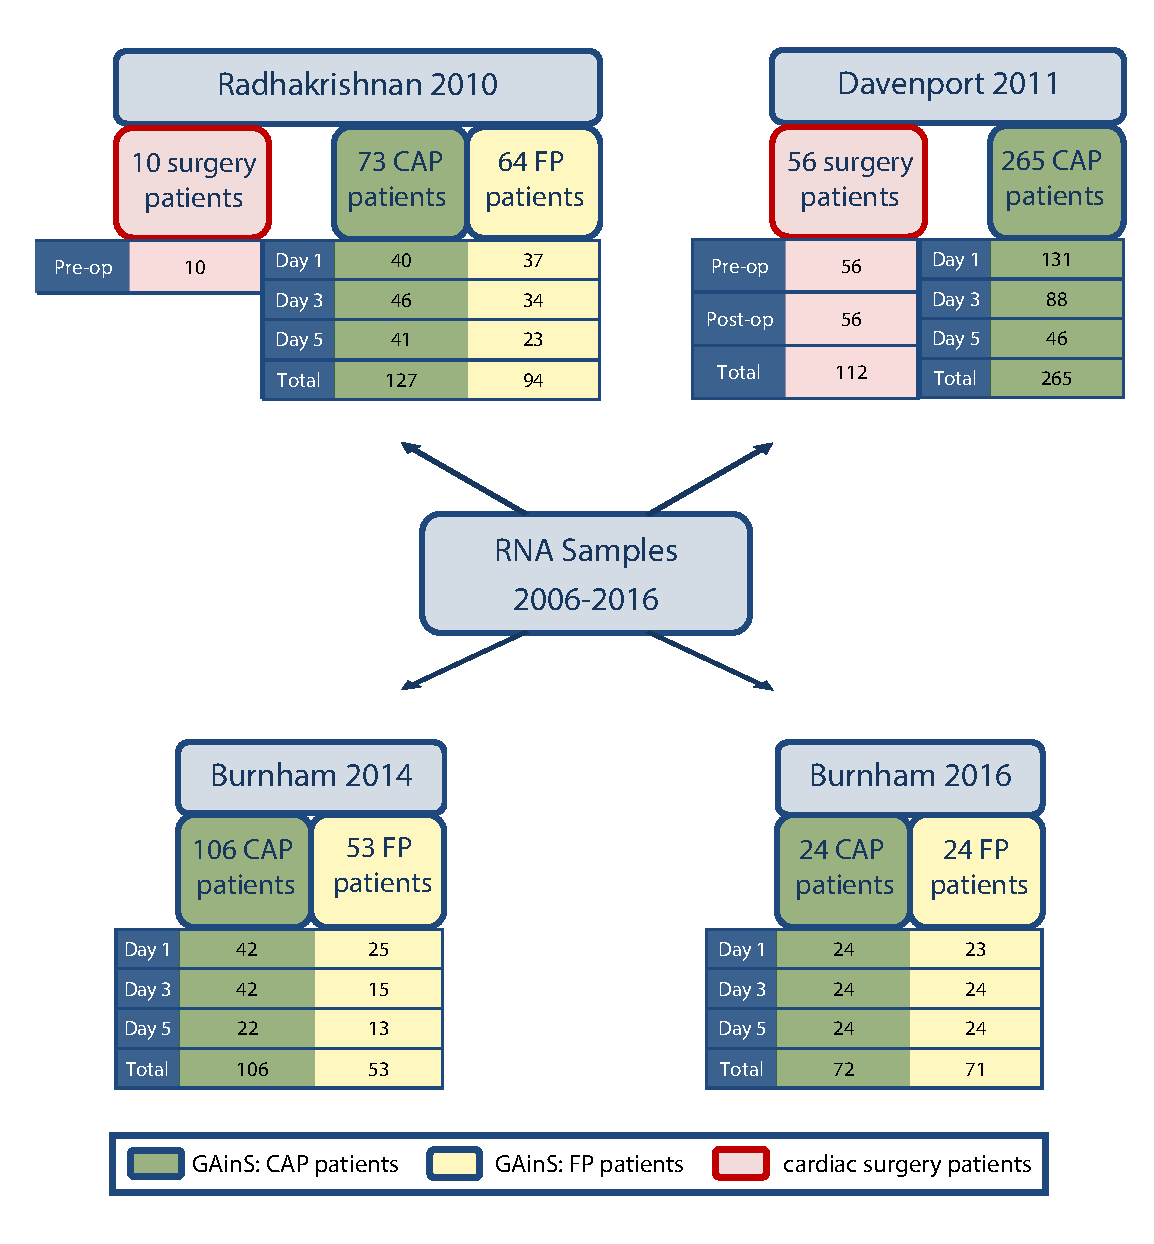
\includegraphics[width=\textwidth]{./Results1/CohortOverview}
\caption[Overview of GAinS gene expression cohorts]{\textbf{Overview of the GAinS gene expression datasets analysed in this thesis.} \\
The number of samples for which gene expression data are available following quality control is given for each of the four cohorts analysed in this thesis. This is subdivided according to the cause of sepsis (CAP (\emph{green}) or FP (\emph{yellow})), given the focus on source of infection in this chapter. Cohorts are named according to the person who generated the data and the year this was done. Samples from elective cardiac surgery patients (\emph{red}), taken before and after their operation by Eduardo Svoren, are also included in the Radhakrishnan 2010 and Davenport 2011 cohorts.}
\label{fig:CohortOverview}
\end{figure}

In this chapter, I analyse sepsis microarray gene expression data processed in several different batches over a six year period (Fig. \ref{fig:CohortOverview}). 

\section{Discussion}

\section{Conclusions}

The analysis presented in this chapter combines multiple transcriptomic datasets to compare the systemic inflammatory response across different sources. This demonstrates that a significant proportion of the sepsis transcriptomic response is shared between CAP and FP patients, although there is some specificity according to infection site. These findings may have implications for the management of sepsis, suggesting patient stratification and targeting treatment on the basis of cause of sepsis could be beneficial. In addition, future research and drug development may benefit from the use of more homogeneous cohorts. However, aspects of the transcriptomic response are shared across sepsis due to CAP and FP and sterile SIRS, indicating that findings in one SIRS subtype might be relevant to another and that similar treatment strategies could be considered. 
\chapter{Improved classification of microbiological aetiology in sepsis}
\label{ch:Results2}
\textit{This chapter explores the diagnosis of microbiological aetiology using various methods}

\startcontents[chapters]{\vspace{-1.4cm}}
\singlespacing
\printcontents[chapters]{}{1}{\section*{ }\setcounter{tocdepth}{1}}
\doublespacing

\section{Introduction}
\subsection{Clinical microbiology of the GAinS CAP cohort}
Of the 1222 patients with sepsis due to CAP in the GAinS cohort, a majority of 729 patients (60\%), were recorded as having no positive microbiology diagnosis (Table ~\ref{tab:clinmicro}). This figure compares similarly to that of the Etiology of Pneumonia in the Community (EPIC) study \parencite{Jain2015} which evaluated CAP requiring hospitalisation among adult patients in the USA and identified 62\% as lacking a microbiology diagnosis. 

\FloatBarrier
\begin{table}[]
\begin{center}
\begin{tabular}{|c|c|l|}
\hline
\multirow{2}{*}{\textbf{Diagnosis}} & \multicolumn{2}{c|}{\textbf{Number of patients (\%)}} \\ \cline{2-3} 
                                    & \textbf{GAinS (n=1222)}    & \textbf{EPIC (n=2259)}   \\ \hline
Unknown                             & 729 (60)                   & 1406 (62)                \\ \hline
Bacterial                           & 399 (33)                   & 247 (11)                 \\ \hline
Viral                               & 80 (7)                     & 530 (23)                 \\ \hline
Mixed bacterial/viral               & 12 (1)                     & 59 (3)                   \\ \hline
Fungal                              & 2 (0.2)                    & 17 (1)                   \\ \hline
\end{tabular}
\end{center}
\smallskip
\caption[Clinical microbiology classification] {\textbf{Microbiological classification for the GAinS (n=1222) and EPIC (n=2259) cohorts.} GAinS data based on curated electronic Case Record Form data. EPIC data obtained from the Etiology of Pneumonia in the Community Study \parencite{Jain2015}.} 
\label{tab:clinmicro}
\end{table}

Interestingly, the GAinS and EPIC cohorts differed in that bacterial infections were predominant in the GAinS cohort (33\%) whereas viral infections were predominant in the EPIC cohort (23\%). The most likely reason for the high viral diagnosis rate in the EPIC cohort is that all patients were systematically tested for viral infections by PCR on nasopharyngeal swabs whereas the GAinS cohort were tested according to clinician judgement. In addition, the higher prevalence of bacterial infections in the GAinS cohort may have been due to a higher severity of illness; GAinS recruited sepsis patients whilst EPIC recruited hospitalised CAP patients.

\subsection{GAinS electronic Case Record Form data}
The CAP microbiology section of the GAinS electronic Case Record Form (eCRF) is divided into three main sections. In this web-based form, research nurses are presented with a series of tick boxes and free text sections relating to:
\begin{enumerate}
	\item The name or category of any identified micro-organism.
	\item The source (sample type) of any identified micro-organism.
	\item Miscellaneous data (e.g. complicating factors such as presence of a pleural effusion, and vaccination status for pneumococcus/influenza).
\end{enumerate}

The eCRF aims to be simple in its format, unfortunately however, it lacks sufficient resolution to enable detailed microbiological phenotyping. For example, the eCRF format doesn't allow for a negative test result to be recorded, this is particularly relevant in the case of molecular testing for viral infections which are frequently not tested for. In addition, the eCRF does not allow for an identified organism to be matched to the source of the positive microbiological test, this is problematic if more than one organism is identified. Furthermore, one tick box option under source of positive microbiological test is "culture of lung secretions" which does not allow differentiation between an expectorated sputum sample and a directed broncho-alveolar lavage sample, samples with very different diagnostic values. The free text boxes of the eCRF often contained valuable clinical microbiology information. Thus, manual curation of the eCRF data was performed.

\subsection{Childhood Meningitis and Encephalitis Study (ChiMES) cohort} 
The targeted metagenomics work was performed in collaboration with the Childhood Meningitis and Encephalitis Study (ChiMES) investigators. ChiMES (http://www.encephuk.org/studies/ukchimes) is a UK-based multi-centre clinical study of over 3000 children with suspected meningitis and encephalitis. A subset of patients (n=243) were included in the targeted metagenomics aspect of the study, consisting of patients with a positive microbiological diagnosis (n=108) and patients without a microbiological diagnosis (n=135). A further control group of meningitis negative individuals (n=22, patients requiring a lumbar puncture for reasons other than meningitis) was studied.

\subsection{Digital droplet PCR (ddPCR)}
Digital droplet PCR (ddPCR) is a method which utilises water-oil emulsion droplet technology. In this technique, a droplet generation step is performed which partitions a 20$\mu$l sample into approximately 20,000 nanolitre-sized droplets. The principle is that each droplet contains one or no copies of the target molecule and the PCR reaction occurs simultaneously in each droplet containing the target molecule. Advantages of ddPCR include absolute quantification without the need for a standard curve (Poisson statistics are employed), increased precision due to the degree of sample partitioning, and increased signal-to-noise ratio where the relative concentration of target to background is low. 

ddPCR was chosen as a method to be applied to the GAinS samples for several reasons. Firstly, it provided an independent method for evaluating the performance of \textit{Castanet}. This is particularly applicable because a clinical microbiological diagnosis of a particular infection type would not necessarily mean the organism was present in plasma, both because the original diagnosis could have arisen from a different specimen type and also because the plasma sampled for metagenomics was collected after antibiotic administration. Secondly, ddPCR provided a quantitative method of assessing pathogen load in plasma.

\subsection{Random forests}
Random forests are supervised machine learning algorithms which are capable of performing both regression and classification tasks. A forest is created which consists of a number of decision trees. Each decision tree sees a subset of the training data (bootstrapping) and at each decision node, a random sample of \textit{m} predictors is chosen from the full set of \textit{p} predictors. For classification tasks, each tree votes for a class and the forest chooses the class which has the most votes by the majority of trees in the forest. Advantages of random forests leading to their suitability for classification tasks based on (meta)genomic data include their ability to handle missing values, their robustness to overfitting, and their ability to handle large datasets with high dimensionality. 

\subsection{Axiom Microbiome Array}
The Axiom Microbiome Array (Affymetrix) is a commercially available platform that enables detection of all organisms in a sample. Organisms are identified at species- or strain-level resolution within a single reaction. The platform is based on microarray technology, with 1,277,846 target probes and 60,152 random negative control probes. The target probes represent 135,555 sequences from 12,513 microbial species from five domains: archaea, bacteria, fungi, protozoa and viruses. 

\subsection{Aims}

To improve microbiological classification of GAinS sepsis patients with CAP through:
\begin{enumerate}
	\item Application of targeted metagenomics to plasma samples
	\item Use of droplet digital PCR (ddPCR) to assay \textit{Streptococcus pneumoniae} and Epstein-Barr Virus from plasma samples
	\item Use of the Axiom Microbiome Array
\end{enumerate}

\section{Results}

\subsection{Targeted metagenomics}
\textbf{Large scale analysis of clinical samples.}
There was successful sequencing of a total of 854 samples, derived from 243 ChiMES meningitis cases, 27 non-meningitis negative-control CSF samples, 573 GAinS sepsis cases, and 11 negative-control plasma samples (Table ~\ref{tab:samples}). The 243 meningitis included 122 patients for which a pathogen had been identified by clinical microbiology (108 from CSF only, plus 14 from a blood sample +/- CSF) and 121 where no pathogen had been identified before sequencing. The sepsis cases comprised 126 for which a pathogen had been identified and 447 chosen for the study because no pathogen had been identified in any relevant sample.

\FloatBarrier
\begin{table}[]
\begin{center}
\begin{tabular}{|c|c|c|c|}
\hline
\multirow{2}{*}{} & \multicolumn{2}{c|}{\textbf{Clinical microbiology}}            & \multirow{2}{*}{\textbf{Negative control}} \\ \cline{2-3}
                  & \textbf{Pathogen identified} & \textbf{No pathogen identified} &                                            \\ \hline
\textbf{ChiMES}   & 122                          & 121                             & 27                                         \\ \hline
\textbf{GAinS}    & 126                          & 447                             & 11                                         \\ \hline
\end{tabular}
\end{center}
\smallskip
\caption[Patient samples sequenced with \textit{Castanet}] {\textbf{Patient samples sequenced with \textit{Castanet}}.) ChiMES and GAinS cases sequenced, including negative control samples.} 
\label{tab:samples}
\end{table}

\textbf{Development of random forest algorithm.}
In order to evaluate the ability of \textit{Castanet} to identify pathogens in real clinical samples, a 'truth dataset' of samples was compiled whose status for particular pathogens was known with confidence. For meningitis cases, the pathogen identified by clinical microbiology testing was accepted as the truth state for microbiology-positive samples. For the 126 pathogen-positive CAP sepsis cases, the pathogen identification had often been made in a sample other than plasma and most of the plasma samples in the collection had been obtained after administration of antibiotics, two situations in which plasma levels of pathogens might have been undetectable by any method. Accordingly, a positive result by ddPCR for \textit{S. pneumoniae} or Epstein-Barr virus (EBV) was used to define a sample subset with which to learn the characteristics of pathogen-true-positive sequencing data. 

Another key issue in interpreting metagenomic sequencing data, especially in large pools of samples, is to distinguish low-level positives from true-negative samples. Here, the \textit{S. pneumoniae} ddPCR assays were used to estimate the threshold for considering a sample sequence-positive. Samples with fewer than either 72 total (specificity 0.94, sensitivity 0.83) or 4 de-duplicated (specificity 0.84, sensitivity 0.85) sequence reads from any single pathogen were excluded from consideration as sequencing-positive (i.e. they were not considered by the random forest algorithm) (Figure \ref{fig:strep-threshold}).

\FloatBarrier
\begin{figure}[htbp]
\centering
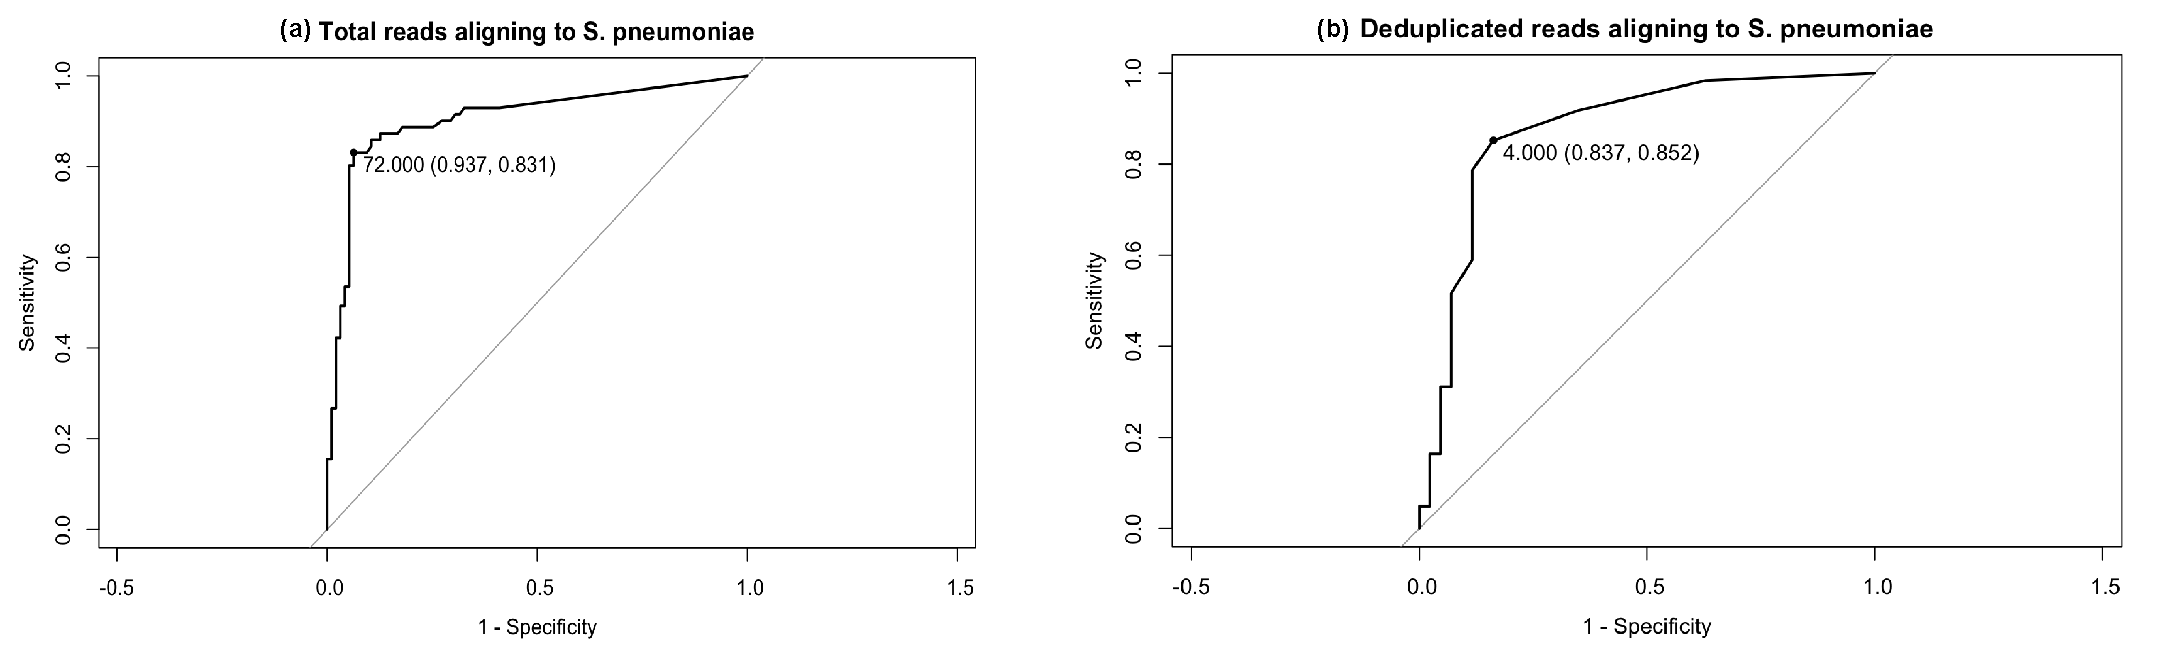
\includegraphics[scale=0.8]{./Results2/Images/strep-threshold.png}
\caption[\textit{S. pneumoniae} detection thresholds]{\textbf{\textit{S. pneumoniae} detection thresholds.} Assessing sample read statistics as predictors of ddPCR-positive status for \textit{S. pneumoniae} detection. ROC curves of (a) total reads and (b) de-duplicated reads as predictors. Youden's J statistic was used to select the respective thresholds of 72 total reads (specificity 0.94, sensitivity 0.83) and 4 de-duplicated reads (specificity 0.84, sensitivity 0.85).}
\label{fig:strep-threshold}
\end{figure}

Combining the above criteria, 100 ChiMES meningitis CSF and 107 GAinS sepsis plasma samples were identified for inclusion as samples with known pathogen status. In addition, negative control samples were included in this cohort (CSF from non-meningitis patients, n=23; plasma from sepsis-negative patients, n=17) to provide instances of pathogen-negative data. Plasma and CSF samples that were microbiology-positive for a particular pathogen were deemed negative for other pathogens. Reads aligning to viruses known to reactivate in sepsis (herpes simplex virus, cytomegalovirus, human herpes virus 6, JC virus) were excluded from the analysis, apart from those EBV samples where ddPCR data was available.

The 247 samples defined above were randomly allocated to training and test datasets in an 80:20 ratio. The training dataset (197 samples: 95 CSF; 102 plasma) were used to train a random forest classifier that used a set of variables derived from the sequencing data to derive a score between 0 and 1 to indicate whether it was positive for each organism with reads in a sample. Most samples contained reads from multiple organisms and the random forest returns a score for each one of these organisms.

The test dataset comprised 50 samples (28 CSF; 22 plasma). A cut-off random forest score of 0.465 was selected for classification of the test set, to appropriately weight specificity over sensitivity (Figure \ref{fig:rf-roc}). At this threshold, there were five false negatives and one false positive in the ChiMES test dataset and one false negative and three false positives in the GAinS test dataset. In the combined set of test samples (Figure ~\ref{fig:rf-test}), the sensitivity was 86.7\% (39 of 45 true positives) and the specificity was 98.6\% (283 of 287 true negatives). Among the most informative sequencing data metrics for prediction were the numbers of total and de-duplicated reads matching a pathogen, taken as the respective proportions of reads aligning to all pathogens in the probeset, and whether a high proportion of the targeted region (regions in the probeset) for that pathogen were covered by reads. 

Since excluding pathogens from a diagnosis can also be clinically useful, the performance of the method in predicting negative status was assessed. With a random forest score threshold of 0.015, 59.2\% of true negatives were correctly identified, with a specificity of 97.8\%, implying that for many samples it is possible to exclude many possible pathogens without erroneously ruling out true positives.

\FloatBarrier
\begin{figure}[htbp]
\centering
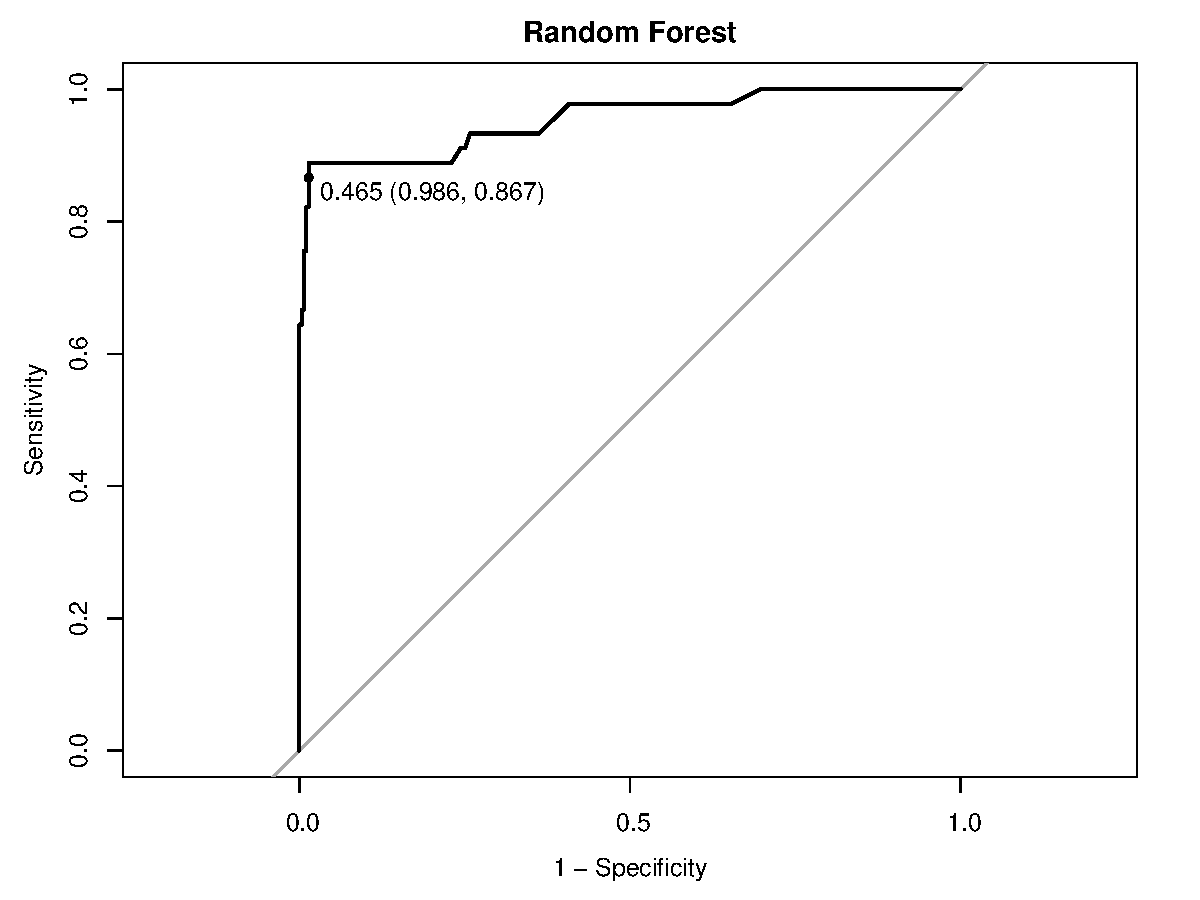
\includegraphics[scale=0.6]{./Results2/Images/rf-roc.pdf}
\caption[Random forest ROC curve]{\textbf{Random forest ROC curve.} ROC curve to choose random forest score threshold for predicting positive samples. A threshold of 0.465 was selected to call samples as positive for a particular pathogen. At this threshold, specificity was 0.986 and sensitivity 0.867.}
\label{fig:rf-roc}
\end{figure}

\begin{figure}[htbp]
\centering
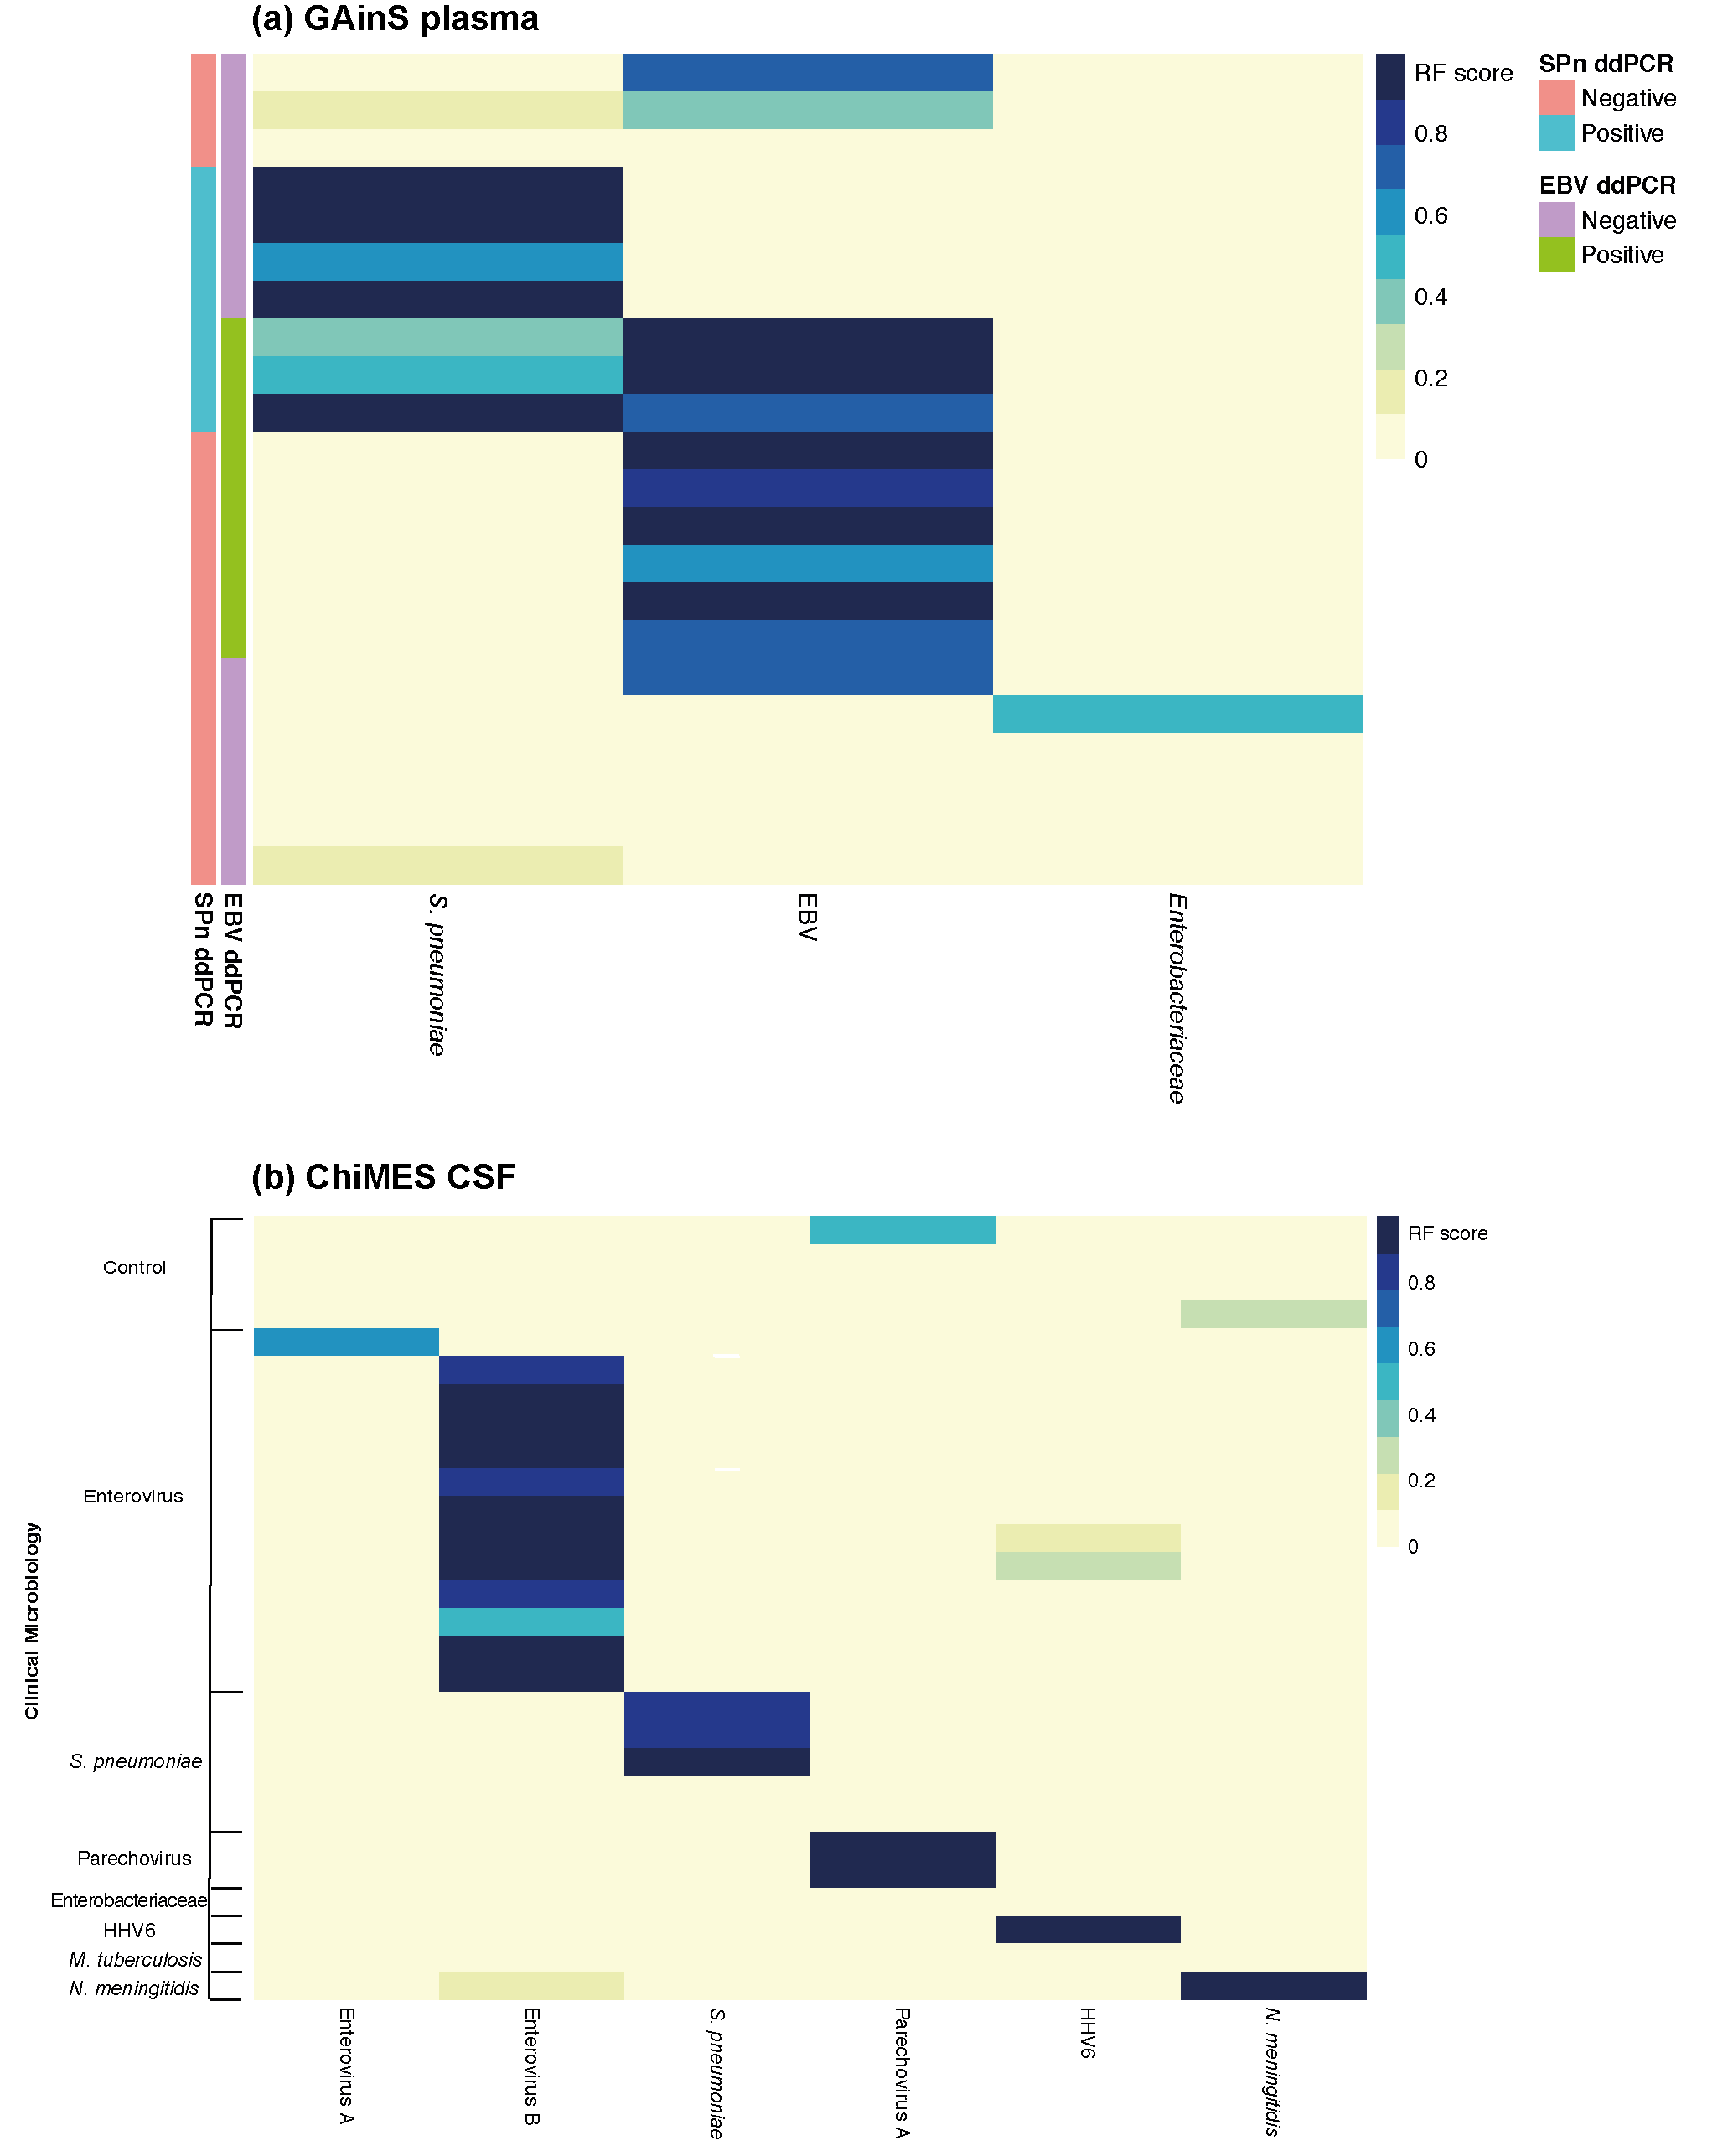
\includegraphics[scale=0.9]{./Results2/Images/rf-test.png}
\caption[GAinS/ChiMES test dataset]{\textbf{GAinS/ChiMES test dataset.} Performance of \textit{Castanet} in clinical samples with a positive microbiology diagnosis. The test dataset included 50 samples: (a) 22 plasma samples (20 GAinS, 2 sepsis-negative controls); (b) 28 CSF samples (24 ChiMES, 4 meningitis-negative controls). The combined overall test dataset specificity and sensitivity was 0.986 and 0.867 respectively. Only organisms detected in each sample set are included as columns in each panel. RF=random forest; HHV6=human herpes virus 6; SPn=\textit{Streptococcus pneumoniae}; EBV=Epstein-Barr Virus; TB=\textit{Mycobacterium tuberculosis}; ddPCR=droplet digital PCR.}
\label{fig:rf-test}
\end{figure}
\FloatBarrier

\textbf{Application to samples with no previous microbiology diagnosis.}
The remaining 447 GAinS sepsis plasma samples, in which no causative pathogen had been identified by routine clinical microbiology, were analysed. \textit{Castanet} identified one or more pathogens in 37\% of samples in sepsis (n=165), including both bacteria and viruses that in many cases were likely to have been causative (Figure ~\ref{fig:rf-unknown}). Among such pathogens, instances of EBV, human herpes virus 6, herpes simplex virus, JC virus and cytomegalovirus in sepsis may represent viral reactivation in the context of critical illness, while \textit{Burkholderia cerpacia} and \textit{Nocardia asteroides} sequences most probably represent contamination of samples \parencite{Salter2014}. Excluding these likely reactivations and contaminants, \textit{Castanet} made 50 new detections in sepsis patients, comprising 11\% of previously unresolved cases (Table ~\ref{tab:gains-unknown}). In the GAinS metagenomic cohort (n=573), \textit{Castanet} improved the overall rate of pathogen identification. \textit{Castanet} identified a likely causative pathogen in 176/573 (31\%) of cases compared with 126/573 (22\%) of cases for clinical microbiology alone (Table ~\ref{tab:gains-summary-castanet}).
 
\begin{figure}[htbp]
\centering
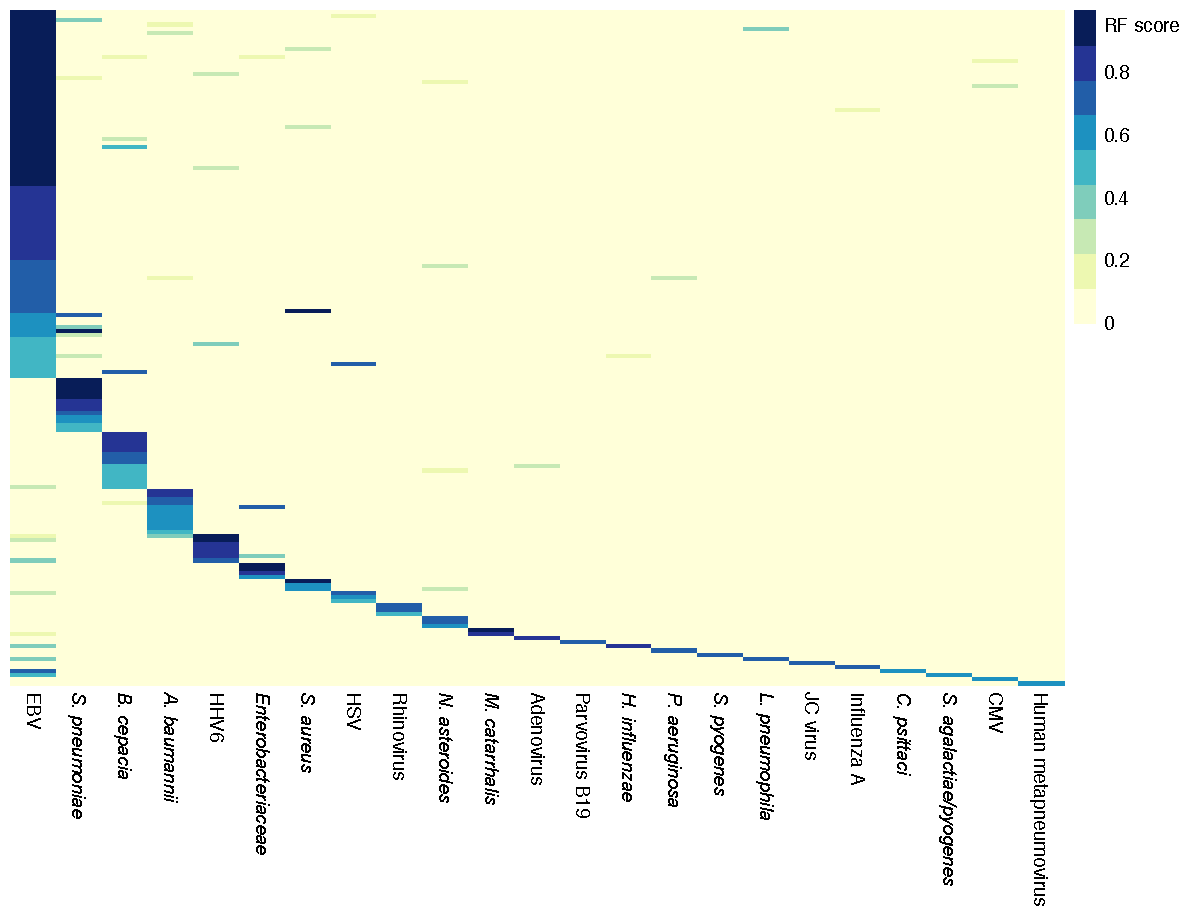
\includegraphics[scale=0.8]{./Results2/Images/rf-gains-unknown.pdf}
\caption[GAinS cases with no clinical microbiology diagnosis]{\textbf{Performance of \textit{Castanet} in cases with no clinical microbiology diagnosis.} Panels show as rows 165/447 GAinS samples; for samples with at least one organism detected at a random forest (RF) score $>$0.465. Only organisms detected in each sample set are included as columns in each panel. EBV=Epstein-Barr virus; HHV6=human herpes virus 6; HSV=herpes simplex virus; CMV=cytomegalovirus}
\label{fig:rf-unknown}
\end{figure}
\FloatBarrier

\begin{table}[]
\begin{center}
\begin{tabular}{|c|c|}
\hline
\textbf{Organism}                 & \textbf{Number of patients} \\ \hline
\textit{Streptococcus pneumoniae} & 16                          \\ \hline
\textit{Acinetobacter baumannii}  & 11                          \\ \hline
\textit{Enterobacteriaceae}       & 5                           \\ \hline
\textit{Staphylococcus aureus}    & 4                           \\ \hline
\textit{Moraxella catarrhalis}    & 2                           \\ \hline
\textit{Haemophilus influenza}    & 1                           \\ \hline
\textit{Pseudomonas aeruginosa}   & 1                           \\ \hline
\textit{Streptococcus pyogenes}   & 1                           \\ \hline
\textit{Legionella pneumophila}   & 1                           \\ \hline
\textit{Chlamydia psittaci}       & 1                           \\ \hline
Rhinovirus                        & 3                           \\ \hline
Adenovirus                        & 1                           \\ \hline
Parvovirus B19                    & 1                           \\ \hline
Influenza A                       & 1                           \\ \hline
Human metapneumovirus             & 1                           \\ \hline
\textbf{Total}                    & \textbf{50}                 \\ \hline
\end{tabular}
\end{center}
\smallskip
\caption[New pathogens identified by \textit{Castanet}] {\textbf{New pathogen identifications made by \textit{Castanet} among sepsis plasma samples.} } 
\label{tab:gains-unknown}
\end{table}

\begin{table}[]
\begin{center}
\begin{tabular}{|c|c|c|c|}
\hline
\textbf{Organism}      & \textbf{\begin{tabular}[c]{@{}c@{}}Clinical \\ microbiology\end{tabular}} & \textbf{\begin{tabular}[c]{@{}c@{}}Clinical microbiology \\ + \textit{Castanet}\end{tabular}} & \textbf{\begin{tabular}[c]{@{}c@{}}Prevalence in \\ overall GAinS cohort\end{tabular}} \\ \hline
Unknown                & 447 (78\%)                                                                & 397 (69\%)                                                                           & 60\%                                                                                   \\ \hline
\textit{S. pneumoniae} & 92 (16\%)                                                                 & 108 (19\%)                                                                           & 15\%                                                                                   \\ \hline
Other bacterial        & 6 (1\%)                                                                   & 33 (6\%)                                                                             & 18\%                                                                                   \\ \hline
Influenza              & 13 (2\%)                                                                  & 14 (2\%)                                                                             & 5\%                                                                                    \\ \hline
Other viral            & 15 (3\%)                                                                  & 21 (4\%)                                                                             & 3\%                                                                                    \\ \hline
\textbf{Total}         & \textbf{573}                                                              & \textbf{573}                                                                         & 100\%                                                                                  \\ \hline
\end{tabular}
\end{center}
\smallskip
\caption[Pathogens identified in all sepsis cases] {\textbf{Pathogens identified in all sepsis cases.} The prevalence of each organism in the overall GAinS cohort (n=1222) based on clinical microbiology is displayed in the last column.} 
\label{tab:gains-summary-castanet}
\end{table}

\subsection{Digital droplet PCR}
\textbf{\textit{Streptococcus pneumoniae}.} ddPCR for the \textit{S. pneumoniae cpsA} gene was performed on the following samples:
\begin{enumerate}
	\item 139 samples from 92 patients with \textit{S. pneumoniae} infection diagnosed by clinical microbiology.
	\item 15 samples from 15 patients with no microbiology diagnosis.
	\item 4 samples from 4 patients with influenza infection diagnosed by clinical microbiology.
\end{enumerate}

ddPCR was performed on the latter two groups of samples for cross-validation because \textit{S. pneumoniae} reads had been unexpectedly identified on metagenomic sequencing. This was prior to the development of the \textit{Castanet} random forest algorithm, thus the remainder of this section will focus only on the ddPCR result from the 92 patients with \textit{S. pneumoniae} infection diagnosed by clinical microbiology.

Of the 139 samples tested, 47 (33.8\%) were positive for \textit{S. pneumoniae}. ddPCR results were compared with \textit{Castanet} sequencing (Table \ref{tab:ddpcr-castanet}). If ddPCR is considered as the gold standard result, this would mean Castanet has a specificity of 100\% and a sensitivity of 83\% for \textit{S. pneumoniae}. There was no significant association between ddPCR positivity and blood culture positivity for \textit{S. pneumoniae} ($\chi^2$=0.13, d.f.=1, p=0.72).

\begin{table}[]
\begin{center}
\begin{tabular}{|l|l|l|l|l|}
\hline
\multicolumn{2}{|l|}{\multirow{2}{*}{}} & \multicolumn{2}{l|}{Castanet} & \multirow{2}{*}{Total} \\ \cline{3-4}
\multicolumn{2}{|l|}{}                  & Negative      & Positive      &                        \\ \hline
\multirow{2}{*}{ddPCR}    & Negative    & 92            & 0             & 92                     \\ \cline{2-5} 
                          & Positive    & 8             & 39            & 47                     \\ \hline
\multicolumn{2}{|l|}{Total}             & 100           & 39            & 139                    \\ \hline
\end{tabular}
\end{center}
\smallskip
\caption[ddPCR and Castanet results for \textit{S. pneumoniae}] {\textbf{ddPCR and Castanet results for \textit{S. pneumoniae}}.) Comparison of results in samples with both ddPCR and \textit{Castanet} data (n=139 samples from n=92 patients).} 
\label{tab:ddpcr-castanet}
\end{table}

\textbf{Epstein-Barr virus.} ddPCR was performed on 619 samples from 565 patients for Epstein-Barr virus (EBV). See Section ~\ref{sssec:ebv}.

\textbf{Influenza virus.} ddPCR was performed for the influenza A matrix gene on 14 plasma samples from 14 patients. All patients had been diagnosed with influenza infection by PCR of a nasopharyngeal swab or respiratory specimen. All samples were negative for influenza via \textit{Castanet} and also tested ddPCR negative. 

\textbf{Relationship between organism load and sequencing yield} Similar to the finding for the five quantified VMR viruses (Figure \ref{fig:vmrconc}), a linear relationship between input pathogen load and sequencing yield was observed in a subset of sepsis plasma samples for which bacterial and viral load of \textit{S. pneumoniae} (n=102) and EBV (n=199) respectively had been quantified by ddPCR (Figure \ref{fig:ddPCR}). Samples where both the ddPCR result and sequencing reads were zero were excluded from the analysis. These findings indicate that the number of de-duplicated reads obtained from targeted enrichment provides data on quantitative yield.

\FloatBarrier
\begin{figure}[htbp]
\centering
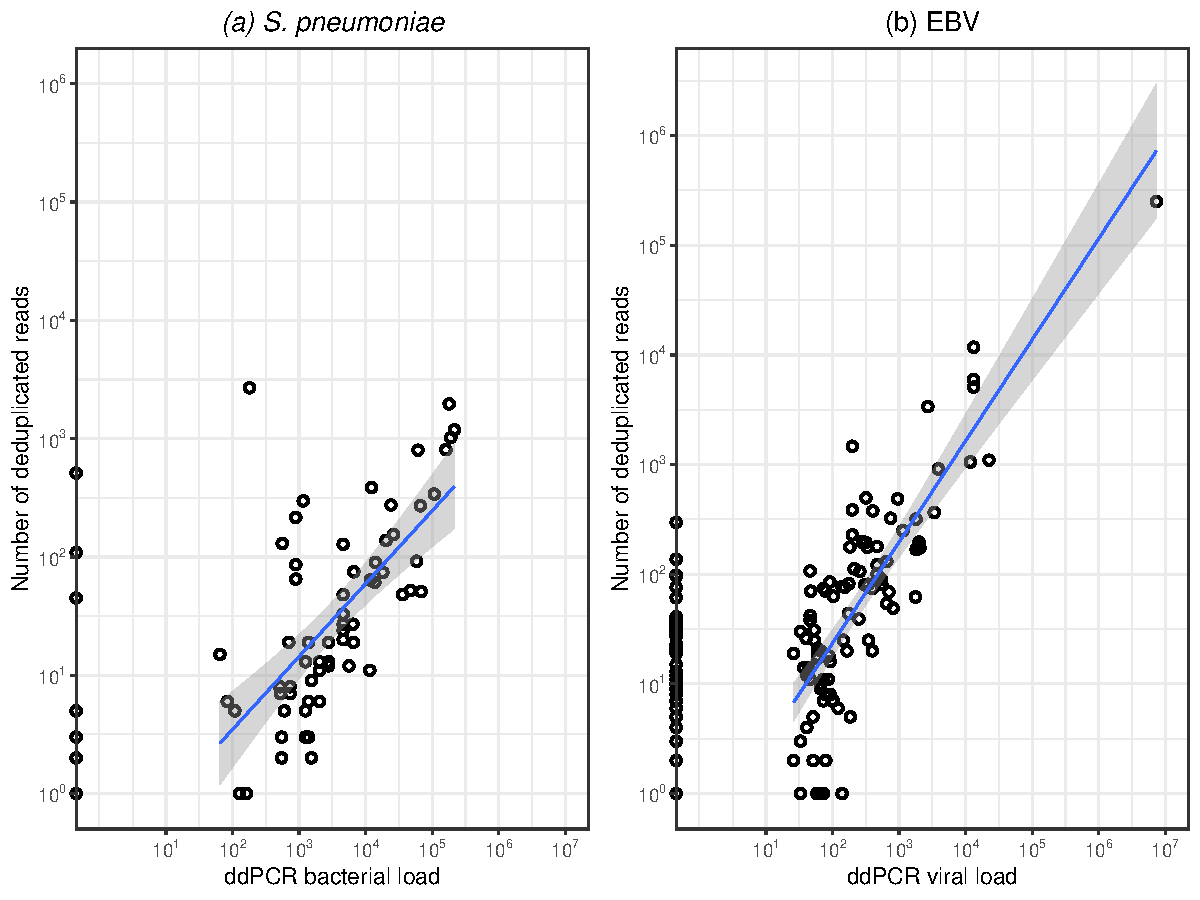
\includegraphics[scale=0.6]{./Results2/Images/ddPCR.pdf}
\caption[Organism load and sequencing yield in sepsis samples]{\textbf{Organism load and sequencing yield in sepsis samples.} De-duplicated read yield was plotted against pathogen load, estimated by ddPCR in samples from a subset of cases in which (a) \textit{Streptococcus pneumoniae} (n=102) or (b) Epstein-Barr virus (EBV) (n=199) was detected by sequencing. A linear relationship between pathogen load and sequencing yield was observed for each organism (\textit{S. pneumoniae}: R$^2$ = 0.449, p = 8.8 x 10$^{-5}$; EBV: R$^2$ = 0.702, p = 2.9 x 10$^{-16}$.}
\label{fig:ddPCR}
\end{figure}

\subsection{Axiom Microbiome Array}
We evaluated plasma from ten patients on the Axiom Microbiome Array platform (Affymetrix). This included four patients with \textit{S. pneumoniae} CAP sepsis, three patients with influenza CAP sepsis, and three uninfected cardiac surgery controls. The Axiom Microbiome Array was evaluated only in terms of detection for DNA-based pathogens as limited sample availability meant that RNA in the samples was not processed (this would have included performing a second assay in parallel, with cDNA synthesis). 

Of the 10 samples, all 4 \textit{S. pneumoniae} sepsis samples were positive for \textit{S. pneumoniae} by \textit{Castanet} sequencing (Figure ~\ref{fig:axiom}). In contrast, the Axiom Microbiome Array platform only detected \textit{S. pneumoniae} was detected in 2 of the 4 samples. When compared with \textit{Castanet} sequencing, the Axiom Microbiome Array platform had a 50\% sensitivity and 100\% specificity for \textit{S. pneumoniae}. 

\FloatBarrier
\begin{figure}[htbp]
\centering
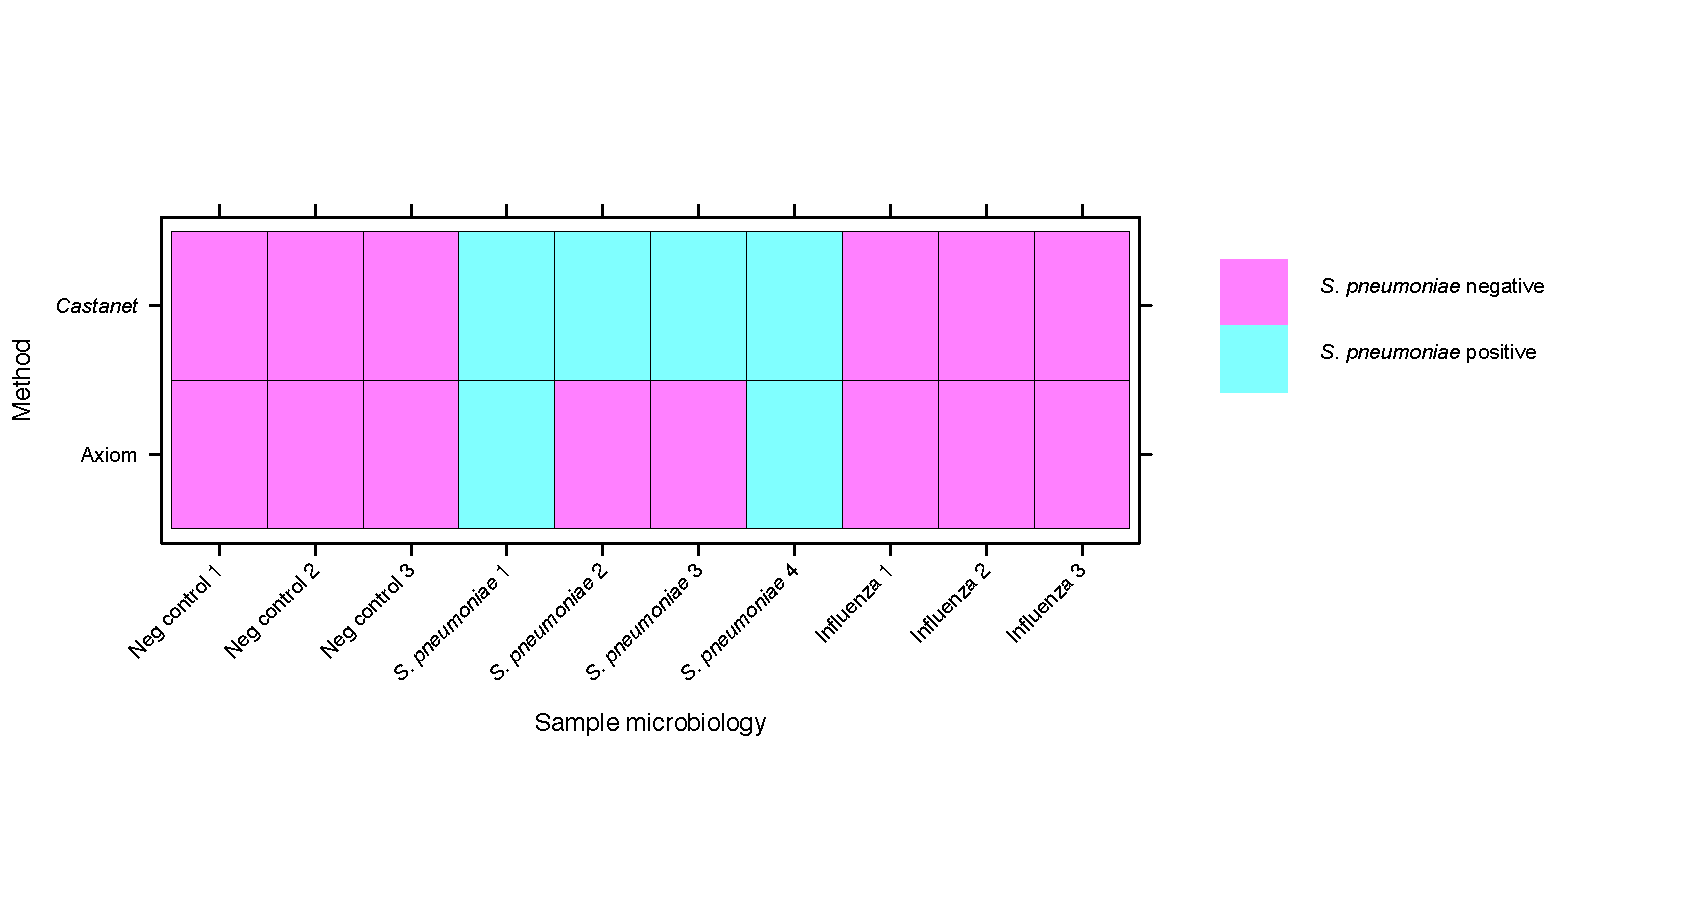
\includegraphics[scale=0.6]{./Results2/Images/Axiom.pdf}
\caption[Axiom Microbiome Array Results]{\textbf{Axiom Microbiome Array results compared with \textit{Castanet}.} Clinical microbiology status and detection for \textit{S. pneumoniae} is displayed in the heatmap.}
\label{fig:axiom}
\end{figure}

In addition, \textit{Escherichia coli} was detected in 9 out of 10 samples, presumably reflecting sample or reagent contamination. Quantitative data is not a feature available via the Axiom Microbial Detection Analysis Software (MiDAS). 

\subsection{Application to the GAinS cohort}
All GAinS patients with no positive microbiology result were analysed by targeted metagenomics if they had a plasma sample available for analysis (n=447/693). In the overall GAinS CAP cohort, the application of targeted metagenomics reduced the number of individuals with no microbiology diagnosis from 729 (60\%) to 693 (57\%). 


\begin{table}[]
\begin{tabular}{|c|c|l|}
\hline
\multirow{2}{*}{\textbf{Diagnosis}} & \multicolumn{2}{c|}{\textbf{Number of patients (\%)}}      \\ \cline{2-3} 
                                    & \textbf{With metagenomics} & \textbf{Without metagenomics} \\ \hline
Unknown                             & 693 (57)                   & 729 (60)                      \\ \hline
Bacterial                           & 426 (35)                   & 399 (33)                      \\ \hline
Viral                               & 86 (7)                     & 80 (7)                        \\ \hline
Mixed bacterial/viral               & 15 (1)                     & 12 (1)                        \\ \hline
Fungal                              & 2 (0.2)                    & 2 (0.2)                       \\ \hline
\end{tabular}
\end{table}
\FloatBarrier


\section{Discussion}
\subsection{Targeted metagenomics and droplet digital PCR}
The \textit{Castanet} workflow enabled successful sequencing of a range of bacteria and viruses (both RNA-based and DNA-based) from a subset of sepsis plasma samples. In spite of difficulties describing a 'truth dataset' of known positives and known negatives, the characteristics of pathogen-positive and pathogen-negative samples were defined using a random forest model that combines data across pathogens and diseases. In the test dataset, a specificity of 98.6\% and sensitivity of 86.7\% was observed. Similarly, high specificity (100\%) and sensitivity (83\%) was also observed when \textit{Castanet} was evaluated against a gold-standard independent method of detection (ddPCR) for \textit{S. pneumoniae}.

Despite this high sensitivity of detection, a causative organism was only identified in 11\% of plasma samples from patients who had no positive microbiology result from routine clinical microbiological testing. This was lower than the figure observed in the ChiMES cohort, where 32\% of similar samples yielded a new diagnosis with \textit{Castanet}. There are several likely explanations for this. Firstly, timing of sample collection was suboptimal for diagnostic metagenomics; the earliest time at which a plasma sample was obtained was on the first day of ICU admission after the consenting process. By this time, the diagnosis of sepsis would have been made and antimicrobial drugs administered. Secondly, the nature of the sample type would have contributed to the low diagnosis rate. In the setting of sepsis secondary to pneumonia, plasma may contain little or no pathogen material from agents such as influenza A virus where viraemia is not typically a feature of disease.

Future work to enable more comprehensive evaluation of \textit{Castanet} sequencing would include recruitment and sampling of patients at earlier time points prior to the administration of antimicrobials, with consent procedures such as emergency waiver of consent in place. In addition, sampling of other relevant specimen types for CAP sepsis (e.g. nasopharyngeal swabs for viral infections) is likely to increase the rate of pathogen detection. 

Other opportunities for future work include improving probe design to enable better resolution of pathogenic species within clusters of closely related bacteria. Currently, \textit{Castanet} is unable to differentiate between species within the \textit{Enterobacteriaceae} family or between \textit{Streptococcus pyogenes} and \textit{Streptococcus agalactiae}. This work could also focus on bacterial sequences of particular clinical interest such as factors associated with virulence and anti-microbial resistance. 

\subsection{Axiom Microbiome Array}
Compared with \textit{Castanet}, the Axiom Microbiome Array had low sensitivity (50\%) for \textit{S. pneumoniae} detection. This may have been because the manufacturers recommend a quantity of 50-100ng DNA per sample which was unachievable in this experiment, given the low DNA quantities (2-20ng) usually obtained following  nucleic acid extraction of the typical 500$\mu$l aliquot of plasma received from the recruiting centres. Other disadvantages include the absence of quantitative data, meaning it was difficult to determine whether the presence of \textit{E. Coli} was as a contaminant or pathogenic. Also, separate workflows (and thus increased sample volumes) are required for RNA and DNA pathogens. These disadvantages outweighed the main benefit of the Axiom Microbiome Array which included the straightforward sample processing, data generation and analysis steps.

For analysis of sample types like plasma from sepsis patients where sensitivity is a major challenge and specimen volumes are limited, the Axiom Microbiome Array is not a suitable method for diagnostics.

\section{Conclusions}
In the GAinS cohort of sepsis CAP patients, the majority of individuals (60\%) lack a microbiological diagnosis despite extensive laboratory testing. In this chapter, I have shown that targeted metagenomics enables new diagnoses to be made in this challenging cohort using the \textit{Castanet} workflow. This has important clinical and scientific implications, enabling more accurate prescribing of antimicrobial therapy and better understanding of disease heterogeneity. 

\chapter{Integration of Microbiology with the Host Response}
\label{ch:Results3}
\textit{This chapter explores the integration of metagenomic data with host transcriptomic and genomic data.}

\startcontents[chapters]{\vspace{-1.4cm}}
\singlespacing
\printcontents[chapters]{}{1}{\section*{ }\setcounter{tocdepth}{1}}
\doublespacing

\section{Introduction}
Application of omics-based methodologies is advancing understanding of the dysregulated host immune response to infection in sepsis. However, the frequently elusive nature of the infecting organism has limited efforts to understand the effect of disease heterogeneity involving the pathogen. This chapter explores how a better understanding of microbiology in the GAinS cohort can be applied to transcriptomic and genomic-based approaches to understand the host response in sepsis. 

\subsection{Immunosuppression in sepsis}
Over the last two decades, there has been a significant shift in our conceptual understanding of immune dysfunction in sepsis. Earlier thinking and sepsis definitions centred around the Systemic Inflammatory Response Syndrome (SIRS) and the corresponding hyperinflammatory and immune activating processes. Now, increasing evidence suggests that immunosuppression is a key disease feature, co-occuring with immune activation, and an important contributor to patient morbidity and mortality \parencite{Daviaud2015}. 

In 2001, Munford and Pugin \parencite{Munford2001} published one of the first studies demonstrating that both pro-inflammatory and anti-inflammatory processes occur rapidly after the onset of sepsis. Later, Boomer and colleagues \parencite{Boomer2011} published further evidence in the form of histological, biochemical and flow cytometric studies documenting defects in immunity in the tissues of patients dying from sepsis. T cell exhaustion, the functional impairment of effector T cells associated with decrease cytokine production, loss of proliferative capacity and decreased cytotoxicity, was described as a key mechanism in sepsis-induced immmunosuppression. 

More recently, transcriptomic studies describing sepsis endotypes have highlighted features of immunosuppression as important in distinguishing endotypes associated with worse outcome \parencite{Davenport2016} \parencite{Scicluna2017}.

\subsection{Sepsis Endotypes}
Previous work in the Knight laboratory \parencite{Davenport2016} describes two sepsis endotypes in the GAinS cohort from genome-wide gene expression analysis of peripheral blood leukocytes. Unsupervised hierarchical cluster analysis of the top 10\% most variable probes (n=2619) was performed on a discovery cohort of 265 GAinS CAP patients. Two groups were identified, Sepsis Response Signature 1 and 2 (SRS1 and SRS2). Individuals with an SRS1 endotype were characterised by features of immunosuppression, including endotoxin tolerance, T-cell exhaustion, and downregulation of HLA class II. Importantly, this group demonstrated higher 14-day mortality (discovery cohort hazard ratio 2.4, 95\% CI 1.3-4.5, p-0.005; validation cohort HR 2.8, 95\% CI 1.5-5.1, p=0.0007), supporting the observation that patients dying of sepsis show marked immunosuppression.

Similar findings were made independently by the MARS consortium \parencite{Scicluna2017}. Sepsis patients admitted to ICUs in the Netherlands were studied and four molecular endotypes (Mars1-4) were described using unsupervised consensus clustering in a discovery cohort of 306 patients from whole blood genome-wide gene expression profiling. Mars1 patients had the worst outcome, with increased 28-day mortality (HR vs all other endotypes 1.86, 95\% CI 1.21-2.86, p=0.0045). Similar to SRS1, this high-risk endotype was characterised immunosuppression, with decreased expression of genes involved in key innate and adaptive immune cell functions.

\subsection{Viral reactivation}
Studies describing a high frequency of viral reactivation in sepsis patients further support the concept that previously immunocompetent individuals can develop a varying degree of functional immunosuppression in response to severe infection. Walton and colleagues observed that 42.7\% of sepsis patients displayed viraemia with more than one reactivated virus \parencite{Walton2014}; the MARS consortium describe a 68\% frequency of herpesvirus viraemia amongst individuals with septic shock \parencite{Ong2017}. 

Reactivated viruses include the herpesviruses Epstein-Barr virus (EBV), cytomegalovirus (CMV), herpes simplex virus (HSV), and human herpesvirus 6 (HHV-6), torque teno virus (TTV), and the polyomaviruses BK and JC virus. In ICU sepsis patients, EBV is the most commonly observed reactivated virus at a frequency of 32-48\% in plasma \parencite{Walton2014} \parencite{Ong2017}. Neither study observed an association with mortality for EBV reactivation alone although the MARS consortium identified a 3.17 HR (95\% CI 1.41-7.13) for mortality with concurrent CMV and EBV reactivation \parencite{Ong2017}. In addition, Walton and colleagues observed an increased incidence of fungal infections, mean SOFA score and ICU length of stay with EBV reactivation \parencite{Walton2014}.

\subsection{Epstein-Barr virus}
Like other herpesviruses, EBV is characterised by its ability to remain dormant in human cells after primary infection. Approximately 90\% of adults worldwide are EBV seropositive \parencite{Cohen2000}, the highest rate of any herpesvirus. 

Following B lymphocyte infection, latency is established with persistent infection arising due to a dynamic balance between viral evasion strategies and host immune responses. Of the 100 genes encoded by the 172Kbp EBV genome, ten are expressed during latency, establishing and maintaining the "immortalized" state. 

Whilst the viral genes and products characterising latency have been well-studied, triggers for the shift from latency to lytic replication and reactivation are not clearly defined. In general, reactivation disease is not believed to be a marked issue with EBV (unlike other herpesviruses, e.g. CMV) apart from in the context of post-transplant lymphoproliferative disorders.

\subsection{Transcriptomic signature of viral infection}
Previous work done in the Knight laboratory by Dr Emma Davenport included the definition of gene expression signatures for different infection types in the GAinS CAP cohort. Four contrasts were made with differentially expressed probes defined as those with a FDR $<$0.05 and a modest fold change $>$1.2. The contrasts made are summarised in Table \ref{tab:emmaDEgenes}. 

\FloatBarrier
\begin{table}[]
\begin{center}
\begin{tabular}{|c|c|l|}
\hline
\textbf{Comparison (no. of patients)} & \textbf{Patients} & \textbf{Differentially expressed probes} \\ \hline
Viral (25) vs no viral (239)          & 264               & 66                                       \\ \hline
H1N1 (16) vs other viral (9)          & 25                & 0                                        \\ \hline
Viral (23) vs bacterial (75)          & 98                & 2                                        \\ \hline
Gram+ (47) vs Gram- (25)              & 72                & 0                                        \\ \hline
\end{tabular}

\end{center}
\smallskip
\caption[Previous work transcriptomic signatures for microbiology] {\textbf{Previous work: differentially expressed probes for microbiology.} Differentially expressed probes defined as those with FDR $<$0.05 and fold change $>$1.2.} 
\label{tab:emmaDEgenes}
\end{table}


Of interest is the viral vs no viral infection  analysis, which identified 66 differentially expressed probes. These mapped to 54 genes in Ingenuity Pathway Analysis (IPA) with enrichment of pathways involving the role of pattern recognition receptors (PRRs) in recognition of viruses and the activation of interferon-regulatory factors (IRF) by cytosolic PRRs.

A prediction model for viral infection was defined using the GeneRave R package (CSIRO Bioinformatics R package version 3.0.8) \parencite{Kiiveri2008}. To reduce the number of possible predictors, only probes that were differentially expressed at FDR $<$0.05 and fold change $>$1.2, mapped to genes in IPA and were moderate to highly expressed (expression $>$6.5) in a proportion of samples equating to the smallest group of the comparison were used. Six genes were selected for the prediction model: \textit{IFI27, TGIF2, LY6E, CCNY, DYNLL2,} and \textit{LAMP3}. Using leave-one-out cross-validation, a ROC curve (AUC 0.89) and MR (9.1) was determined for the model.

Limitations of this analysis include the lack of accurate microbiological phenotyping in the comparator "non-viral" group. The electronic case record forms (eCRF) only provides information where testing yields a positive result, thus we are unable to confirm cases where testing has yielded a negative result. As viral testing is typically only performed during influenza outbreaks, there is a high likelihood the "non-viral" group included cases of undiagnosed viral infection. This may explain why only 66 differentially expressed probes were identified at a modest fold change of 1.2. 


\subsection{HLA}
The extreme variability seen in the Major Histocompatibility Complex (MHC) region is believed to have arisen due to human-viral co-evolution. It is unsurprising therefore, that associations are seen between specific HLA alleles and infectious disease susceptibility, progression and outcome. 

Notable examples include human immunodeficiency virus 1 (HIV-1), hepatitis B virus (HBV) and hepatitis C virus (HCV) infection. In HIV-1 infection, Carrington and colleagues \parencite{Carrington1999} tested 63 alleles and found six (A*29, B*27, B*35, B*41, Cw*04 and Cw*12) to be significantly associated with disease progression in Caucasians. In HBV infection, Nishida and colleagues \parencite{Nishida2016} tested 144 alleles and found DQB1*06:01 to have the strongest association with susceptibility to chronic infection in Japanese individuals. Finally, in HCV infection, B*27 \parencite{Neumann-Haefelin2006} and B*57 \parencite{Kim2011} have both been found to be associated with a higher rate of viral clearance. 

In addition, genome-wide association studies (GWAS) and genome-wide linkage studies (GWLS) have identified polymorphisms in the HLA regions to be associated with viral (HIV, HBV, HCV), bacterial (leprosy, tuberculosis), and parasitic (malaria, leishmaniasis, and schistosomiasis) infections \parencite{Blackwell2009}. For example, the International HIV Controllers Study \parencite{Pereyra2010} identified over 300 genome-wide significant SNPs within the MHC to be associated with control of HIV-1 whilst the first GWAS of leprosy susceptibility reported associations with SNPs in six genetic loci, including the HLA-DR region \parencite{Zhang2009}.  

In summary, these examples in the literature suggest it would be of particular interest to investigate the association between specific HLA alleles and susceptibility to different microbiological classes of sepsis. 

\subsection{Aims}

\begin{enumerate}
	\item To characterise the extent and implications of EBV reactivation and integrate this with host transcriptomic data.
	\item To investigate the association between \textit{Streptococcus pneumoniae} bacterial load and sepsis endotype (SRS status).
	\item To describe host transcriptomic signatures of viral infection, influenza infection, and \textit{Streptococcus pneumoniae} infection.
	\item To investigate the association between host genotype (HLA type) and susceptibility to different classes of infection.
\end{enumerate}

\section{Results}
\subsection{Combination of microarray datasets}
In this chapter, I analyse microarray gene expression data processed in four batches over a six year period. These include samples from patients with sepsis due to CAP or faecal peritonitis (FP) enrolled through the GAinS study, recruited from 34 participating ICUs between 2005 and 2016. Serial samples were obtained on the first, and/or third, and/or fifth day of ICU admission. The total peripheral blood leukocyte population was isolated from whole blood for RNA extraction using the LeukoLOCK system (Invitrogen).

All four of these datasets were generated by former DPhil students in the Knight lab: Radhakrishnan 2010, Dr Jayachandran Radhakrishnan; Davenport 2011, Dr Emma Davenport; Burnham 2014, Dr Katie Burnham; Burnham 2016, Dr Katie Burnham. Samples from cardiac surgery patients (sepsis control patients) were taken prior to and after their operation, and included in the two earlier cohorts. These samples were processed by Dr Eduardo Svoren (Barts and the London).

Genome-wide gene expression data was generated for all four cohorts using the Illumina Human-HT-12 v4 Expression BeadChip (47,231 probes). The data QC and normalisation was performed for each dataset in parallel. This was performed by myself for the Radhakrishnan 2010 and Davenport 2011 datasets, and by Dr Katie Burnham for the Burnham 2014 and Burnham 2016 datasets. Table \ref{tab:gex-summary} summarises the samples included in each dataset following QC. Following QC of each dataset, the four datasets were combined.

\begin{table}[]
\begin{center}
\begin{tabular}{|l|l|l|l|l|}
\hline
\textbf{Dataset}   & \textbf{\begin{tabular}[c]{@{}l@{}}Samples \\ post-QC\end{tabular}} & \textbf{CAP}    & \textbf{FP}   & \textbf{Cardiac} \\ \hline
Radhakrishnan 2010 & 236                                                                 & 124 (39/45/40)  & 94 (37/34/23) & 18 (6/6/6)       \\ \hline
Davenport 2011     & 339                                                                 & 262 (130/86/46) & 0             & 77 (39/0/38)     \\ \hline
Burnham 2014       & 159                                                                 & 106 (42/42/22)  & 53 (25/15/13) & 0                \\ \hline
Burnham 2016       & 143                                                                 & 72 (24/24/24)   & 71 (23/24/24) & 0                \\ \hline
\textbf{Total}     & \textbf{877}                                                        & \textbf{564}    & \textbf{218}  & \textbf{95}      \\ \hline
\end{tabular}
\end{center}
\smallskip
\caption[Summary of microarray datasets]{\textbf{Summary of microarray datasets}. Numbers in brackets refer to samples at each timepoint. The three timepoints for the sepsis patients are day 1, day 3 and day 5 after ICU admission. The three timepoints for the cardiac surgery patients are pre-operative, immediately post-operative, 24 hours post-operative.}
\label{tab:gex-summary}
\end{table}

\textbf{Radhakrishnan 2010}
The Radhakrishnan 2010 dataset (n=264) \parencite{Radhakrishnan2012} included 234 samples from 138 sepsis patients and 30 samples from 10 cardiac surgery patients. Twenty-two samples were excluded prior to data normalisation (3 samples from a patient subsequently discovered as failing to meet study inclusion criteria; 2 mislabelled samples; 5 technical replicates; 12 samples from cardiac surgery patients with missing consent forms). 

Six outlying samples were identified through Principal Component Analysis (PCA and other QC measures (Figure \ref{fig:PCAJay}) and excluded. Probes that did not have a detection p-value $<$0.05 in at least 5\% of samples were removed (19,978 probes). Following normalisation and QC, expression data was available for 27,253 probes in 236 samples (124 CAP, 94 FP, 18 cardiac surgery) from 143 patients (73 CAP, 64 FP, 6 cardiac surgery).

\FloatBarrier
\begin{figure}[htbp]
\centering
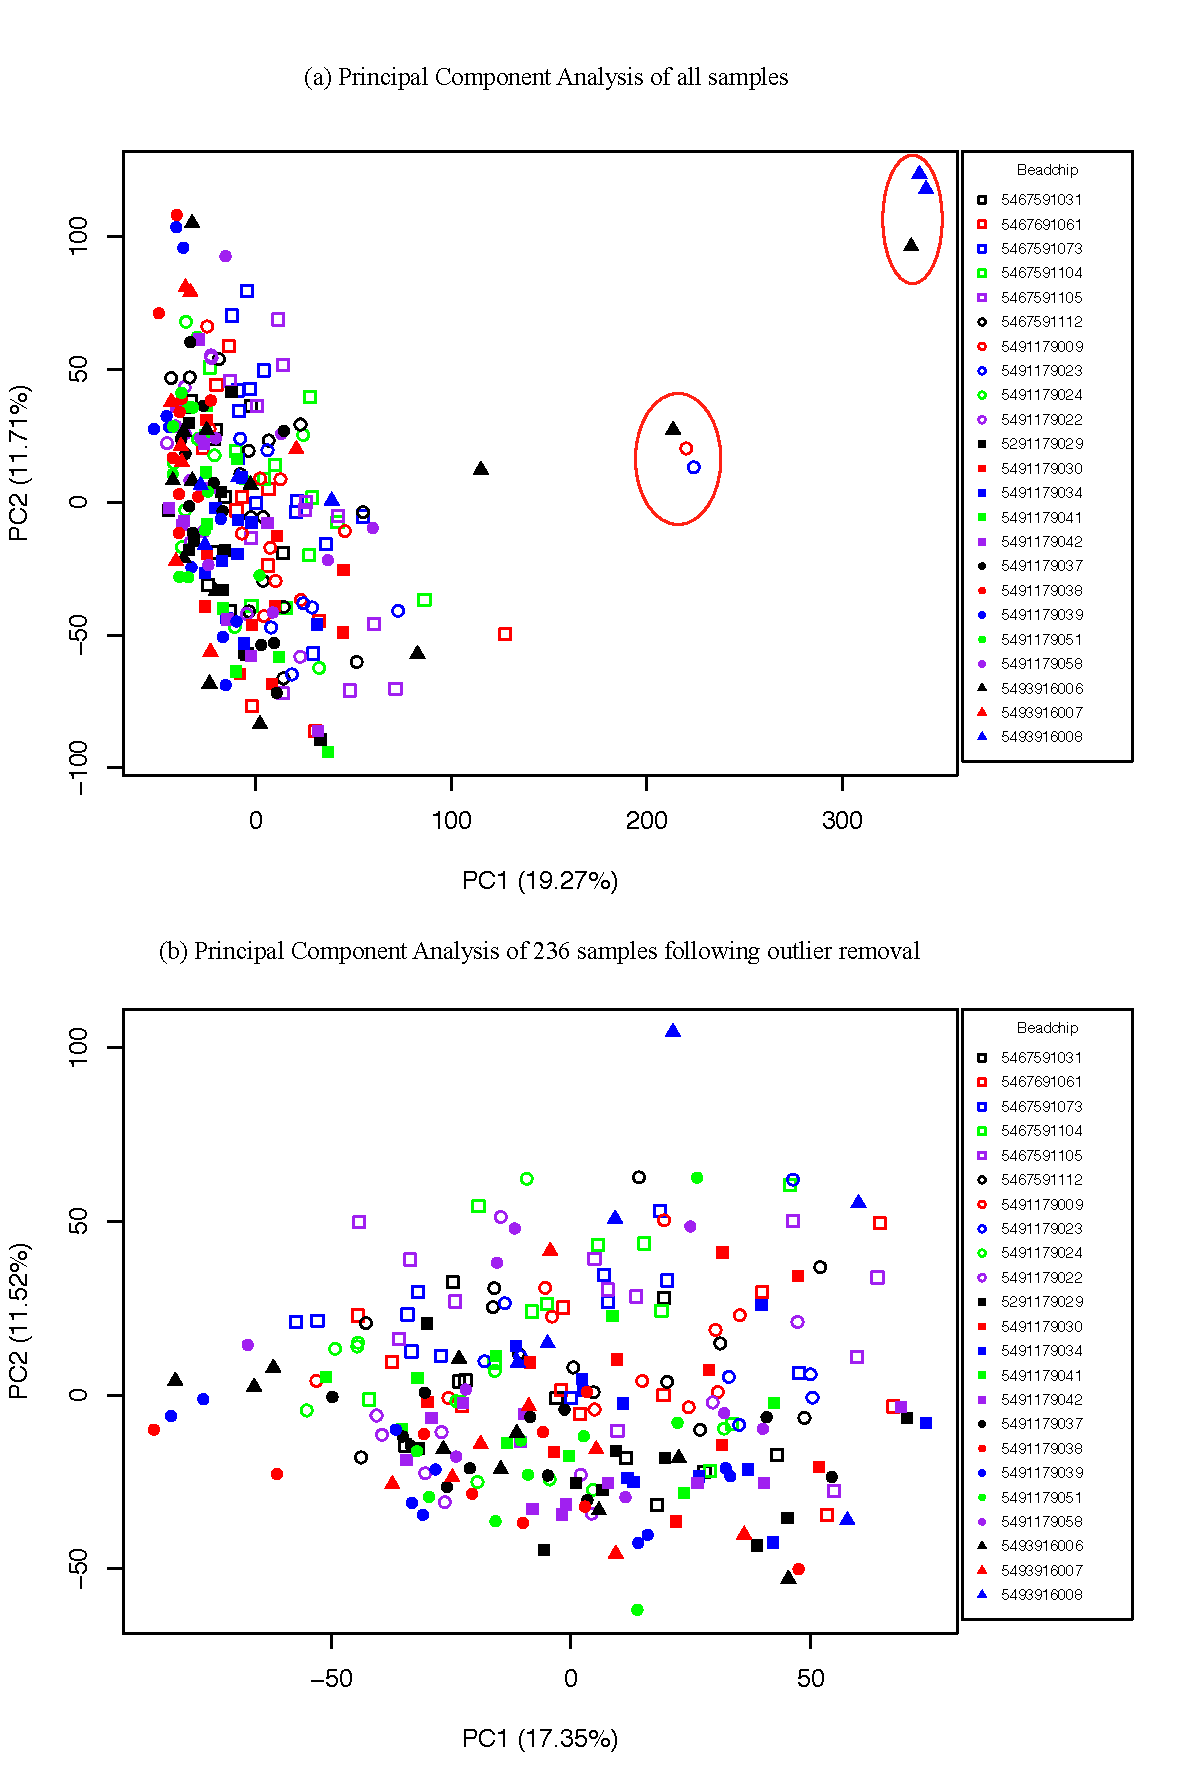
\includegraphics[scale=0.7]{./Results3/Images/PCA_Radhakrishnan2010.pdf}
\caption[Principal Component Analysis: Radhakrishnan 2010]{\textbf{Principal Component Analysis: Radhakrishnan 2010} The first two principal components of the gene expression data are plotted, with the amount of variance explained by each noted; (a) when all samples are included in the analysis, and (b) after the removal of six outliers. Samples are coloured according to beadchip and outlying samples are circled in red.}
\label{fig:PCAJay}
\end{figure}

\textbf{Davenport 2011}
The Davenport 2011 dataset has been published as the discovery cohort in \cite{Davenport2016}. This initial dataset (n=432) included 306 samples from 306 CAP patients and 126 samples from 63 cardiac surgery patients. Eighty-five samples were excluded prior to data normalisation (48 samples from 4 chips with failed hybridisation; 34 samples from cardiac surgery patients with missing consent forms; 1 patient subsequently discovered as failing to meet study inclusion criteria; 1 patient who withdrew consent; 1 patient with suspected active leukaemia). 

Eight outlying samples were identified through PCA and other QC measures (Figure \ref{fig:PCAEmma}) and excluded. Probes that did not have a detection p-value $<$0.05 in at least 5\% of samples were removed (20,805 probes). Following normalisation and QC, expression data was available for 26,426 probes in 339 samples (262 CAP, 77 cardiac surgery) from 301 patients (262 CAP, 39 cardiac surgery).

\FloatBarrier
\begin{figure}[htbp]
\centering
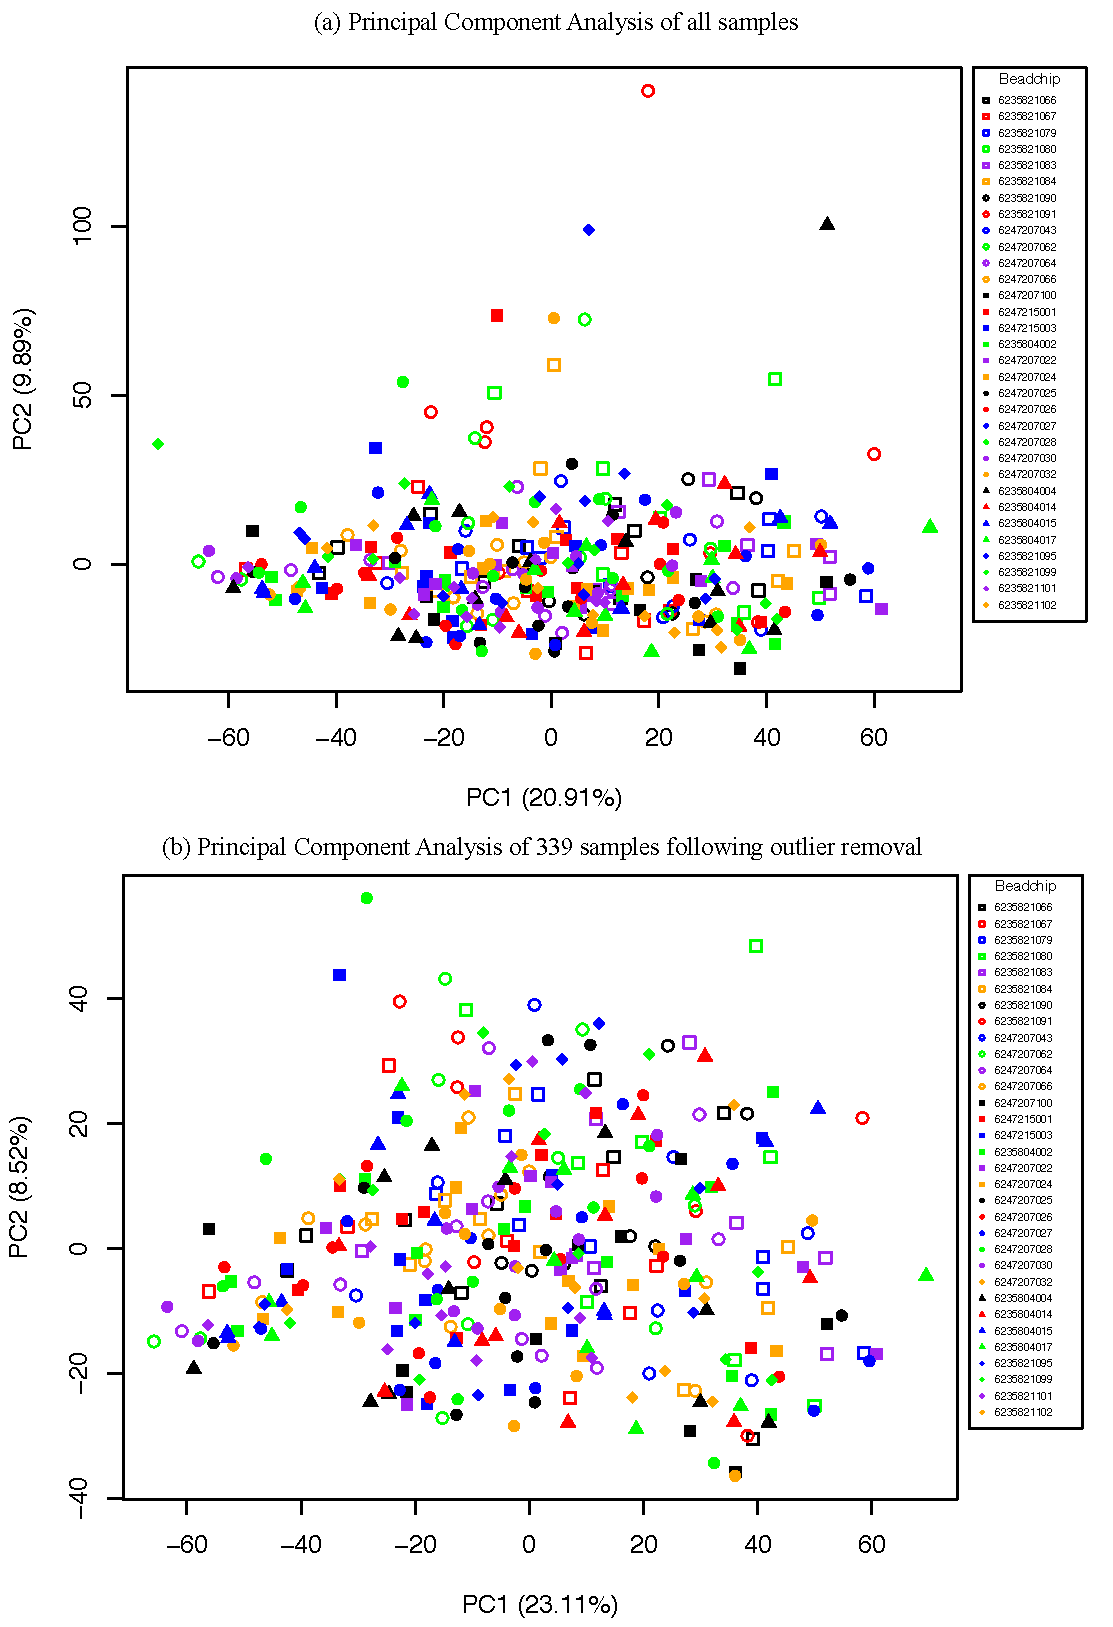
\includegraphics[scale=0.7]{./Results3/Images/PCA_Davenport2011.pdf}
\caption[Principal Component Analysis: Davenport 2011]{\textbf{Principal Component Analysis: Davenport 2011} The first two principal components of the gene expression data are plotted, with the amount of variance explained by each noted; (a) when all samples are included in the analysis, and (b) after the removal of eight outliers. Samples are coloured according to beadchip and outlying samples are circled in red.}
\label{fig:PCAEmma}
\end{figure}

\textbf{Burnham 2014}
Data QC and normalisation was carried out by Dr Katie Burnham \parencite{Burnham2017}. Post-QC, this dataset was comprised of 159 samples (106 CAP, 53 FP) from the same number of patients.

\textbf{Burnham 2016}
Data QC and normalisation was carried out by Dr Katie Burnham \parencite{Burnham2017}. Post-QC, this dataset was comprised of 143 samples (72 CAP, 71 FP) from 48 patients (24 CAP, 24 FP).

\textbf{Combination of datasets}
Following separate QC and normalisation, the four datasets were combined. There were 92 additional probes in the two more recent datasets, which were removed. In addition, there were 61 samples that were repeated in the Davenport 2011 dataset following initial analysis in the Radhakrishnan dataset. Given that the SRS endotypes were defined and published for the Davenport 2011 dataset, the samples in this dataset were retained and duplicates in the Radhakrishnan 2010 dataset removed. Probes that did not have a detection p-value $<$0.05 in at least 5\% of samples were removed (19,003 probes). Data was then normalised before the ComBat function from the R package sva applied to remove known batch effects (Figure \ref:fig{combat}). In this combined dataset, expression data was available for 28,228 probes for 816 samples (509 CAP, 218 FP, 89 cardiac surgery) from 591 patients (408 CAP, 141 FP, 42 cardiac surgery).

\FloatBarrier
\begin{figure}[htbp]
\centering
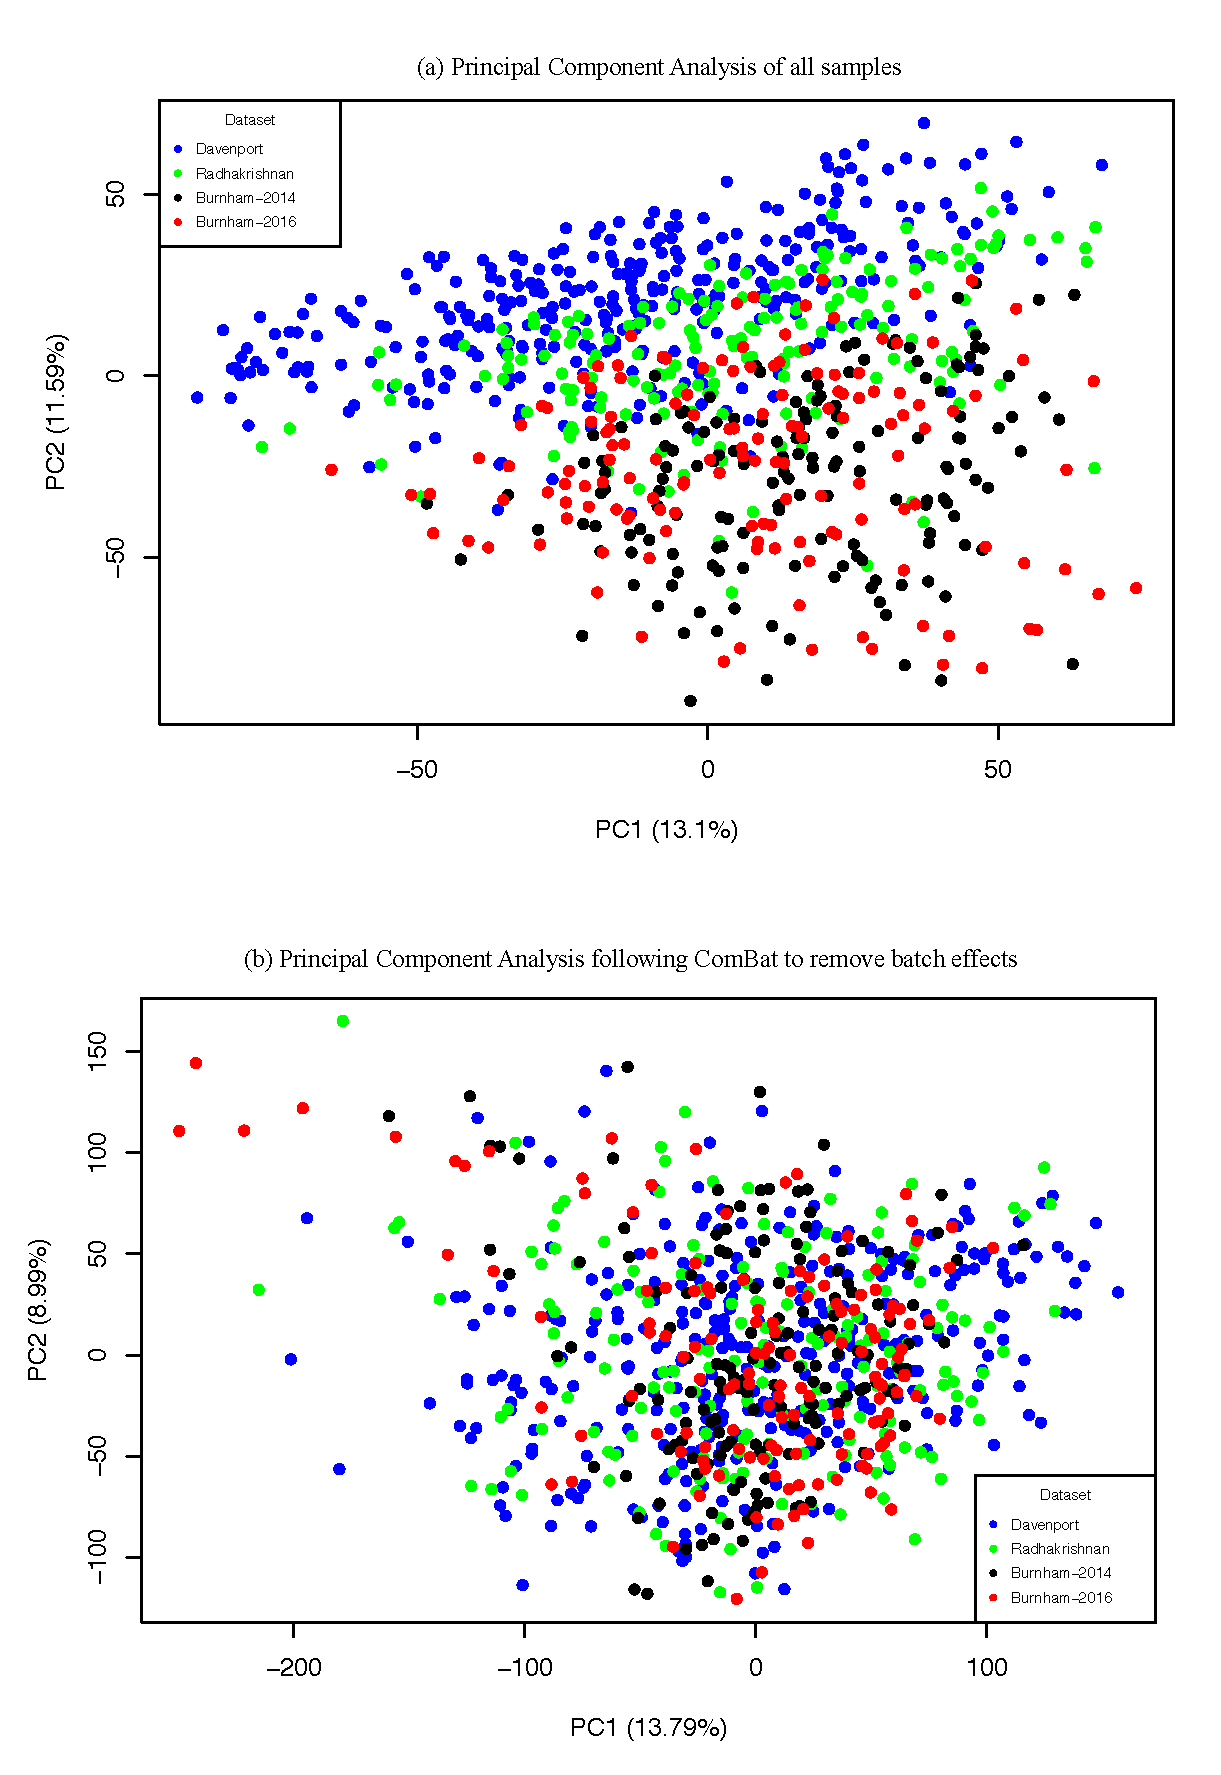
\includegraphics[scale=0.7]{./Results3/Images/PCA_alldata.pdf}
\caption[Principal Component Analysis: Combined dataset]{\textbf{Principal Component Analysis: Combined dataset} The first two principal components of the gene expression data are plotted, with the amount of variance explained by each noted; (a) prior to batch effects being removed (b) after removal of batch effects by ComBat. Samples are coloured according to dataset.}
\label{fig:combat}
\end{figure}

\subsection{Evidence for immunosuppression: viral reactivation}
Amongst 757 samples from 573 patients undergoing metagenomic sequencing (the metagenomic cohort), viral reactivation was observed in 24\% of individuals, with EBV the most commonly observed virus (Table ~\ref{tab:viralreactivation}). Notably, this was observed despite there being an enrichment for earlier time points from ICU admission (Day 1=302; Day 3=284; Day 5=171). Six individuals showed simultaneous reactivation of EBV and a second virus. 

\begin{table}[]
\begin{center}
\begin{tabular}{|c|c|c|c|c|c|}
\hline
\begin{tabular}[c]{@{}c@{}}Other reactivated\\ virus\end{tabular} & None       & HSV       & CMV       & HHV-6     & JC virus  \\ \hline
\begin{tabular}[c]{@{}c@{}}EBV-negative \\ (n=438)\end{tabular}   & 422 (74\%) & 5 (0.9\%)                                                      & 1 (0.2\%)       & 8 (1.4\%)                                                      & 2 (0.3\%) \\ \hline
\begin{tabular}[c]{@{}c@{}}EBV-positive\\ (n=135)\end{tabular}    & 129 (23\%) & 4 (0.7\%)                                                      & 1 (0.2\%)       & 0 (0\%)                                                        & 1 (0.2\%) \\ \hline
\end{tabular}
\end{center}
\smallskip
\caption[Incidence of viral reactivation]{\textbf{Incidence of viral reactivation in the metagenomic cohort (n=573)}. Six patients demonstrated reactivation with EBV and a second virus.}
\label{tab:viralreactivation}
\end{table}
\FloatBarrier

As the incidence of CMV reactivation was unexpectedly low, droplet digital PCR was carried out on a subset of samples overlapping with the metagenomic cohort (n=98). Samples were selected based on: (a) host transcriptomic data availability (overlap with Davenport 2011 cohort); (b) CMV positivity from metagenomics (n=1); and (c) sample availability. Of the 98 samples assayed, only two were positive for CMV including the one positive sample identified by metagenomics. The second sample (missed by metagenomics) was positive for CMV at a low level (86 copies/ml).

\subsection{Evidence for immunosuppression: EBV}
\label{sssec:ebv}
\textbf{Cohort description.}
EBV was assayed from plasma samples taken at one or more time points (day 1 and/or day 3 and/or day 5 of ICU admission) by two methods, targeted metagenomics (757 samples from 573 patients) and digital droplet PCR (ddPCR) (619 samples from 565 patients), forming the two cohorts for this section. Targeted metagenomics enabled characterisation of multiple reactivated viruses in plasma, whilst ddPCR enabled a quantitative approach focused on EBV, enabling assessment of individuals from the metagenomic cohort at later time points as well as additional individuals. There was an overlap of 409 patients in the application of the two methods, with a total of 731 patients evaluated overall.

\textbf{Serology.}
Plasma from 40 EBV ddPCR-positive patients, selected to represent the full range of viral loads observed, were tested for IgG and IgM antibodies against EBV Viral Capsid Antigen (VCA). All individuals tested (n=40; 100\%) were positive for the IgG VCA antibody and negative for IgM VCA antibody, indicating that sepsis had coincided with viral reactivation and not primary infection.

\textbf{Incidence of reactivation with time after ICU admission.}
Combining both cohorts, a total of 1042 unique samples (731 patients) from days 1,3 and 5 after ICU admission were evaluated by either targeted metagenomics, ddPCR, or both. Where the ddPCR and metagenomic result differed (15\% of samples), the positive result was taken forward for further analysis. The overall incidence of EBV reactivation at any time point was 37\% (271/731). The incidence of EBV reactivation increased significantly over time ($\chi^2$=24.6; d.f.=2; p=4.6 x 10$^{-6}$) (Table ~\ref{tab:ebvincidence}).

\FloatBarrier
\begin{table}[]
\begin{center}
\begin{tabular}{|c|c|c|c|}
\hline
\textbf{Day of sampling} & \textbf{EBV negative} & \textbf{EBV positive} & \textbf{Total} \\ \hline
1                        & 245 (75\%)            & 82 (25\%)             & 327            \\ \hline
3                        & 247 (70\%)            & 106 (30\%)            & 353            \\ \hline
5                        & 209 (58\%)            & 153 (42\%)            & 362            \\ \hline
\end{tabular}
\end{center}
\smallskip
\caption[EBV status by day of sampling]{\textbf{EBV status by day of sampling after ICU admission}}
\label{tab:ebvincidence}
\end{table}

\textbf{Clinical outcomes.}
Clinical outcome data was compared between EBV-negative (n=460) and EBV-positive (n=271) individuals (Table ~\ref{tab:ebvoutcome}); patients were considered EBV-positive if at least one sample at any time point was positive by ddPCR or targeted metagenomics. Twenty-eight-day mortality was higher (27\% vs 20\%; p=0.04) and ICU length of stay was longer (12.9 days vs 9.2 days; p=0.004) in the EBV-positive group. In addition, the EBV-positive group had more organ failures with higher day 1 Sequential Organ Failure Assessment (SOFA) scores (6.9 vs 5.9; p=0.00011) and maximum SOFA scores (7.9 vs 6.7; p=3.6 x 10$^{-6}$).

\begin{table}[]
\begin{center}
\begin{tabular}{|c|c|c|c|}
\hline
\textbf{Characteristic}     & \textbf{\begin{tabular}[c]{@{}c@{}}EBV-negative\\ (n=460)\end{tabular}} & \textbf{\begin{tabular}[c]{@{}c@{}}EBV-positive\\ (n=271)\end{tabular}} & \textbf{p-value} \\ \hline
Age                         & 60.5 (17-92)                                                            & 62.4 (19-91)                                                            & 0.11             \\ \hline
Male sex\textasciicircum{}  & 275 (60\%)                                                              & 141 (52\%)                                                               & 0.049             \\ \hline
Mortality (28-day)`         & 92 (20\%)                                                               & 72 (27\%)                                                               & 0.040             \\ \hline
ICU length of stay`         & 9.2 & 12.9 & 0.0040            \\ \hline
SOFA score (day 1)*         & 5.9 & 6.9 & 0.00011           \\ \hline
SOFA score (maximum)*       & 6.7 & 7.9                                                                     & 3.6 x 10$^{-6}$           \\ \hline
\end{tabular}
\end{center}
\smallskip
\caption[EBV and clinical outcomes]{\textbf{Clinical characteristics and outcome data compared between EBV-negative and EBV-positive individuals (total n=731).}ICU length of stay analysis only includes patients surviving to ICU discharge. T-test performed except where indicated (\textasciicircum{}Chi-squared test; *Mann-Whitney U-test; `Log-rank test).} 
\label{tab:ebvoutcome}
\end{table}
\FloatBarrier

\textbf{Association with SRS endotype.} 
SRS group membership (determined at the first available time point after ICU admission) was evaluated in the context of EBV positivity over the first 5 days of ICU admission. Considering SRS endotype as a categorical trait, there was a greater proportion of SRS1 patients within the EBV-positive group (44\% vs 35\%; p=0.097) but this was not statistically significant (Table ~\ref{tab:ebv-gex}). However, this binary classification is a simplification of what is a continuous spectrum of gene expression patterns, with some individuals at either extreme and others with more moderate SRS signatures in the centre. Therefore, we reasoned that considering SRS endotype as a continuous trait might increase statistical power to detect an association with EBV-positivity.

\begin{table}[]
\begin{center}
\begin{tabular}{|c|c|c|c|}
\hline
\textbf{Characteristic}                       & \textbf{\begin{tabular}[c]{@{}c@{}}EBV-negative \\ (n=239)\end{tabular}} & \textbf{\begin{tabular}[c]{@{}c@{}}EBV-positive \\ (n=152)\end{tabular}} & \textbf{p-value} \\ \hline
Age                                           & 63.5 (19-91)                                                             & 63.5 (17-91)                                                             & 1.00             \\ \hline
Male sex\textasciicircum{}                    & 149 (62\%)                                                               & 88 (58\%)                                                                & 0.44             \\ \hline
Sepsis Response Signature 1\textasciicircum{} & 84 (35\%)                                                                & 67 (44\%)                                                                & 0.097            \\ \hline
Mortality (28-day)'                           & 69 (29\%)                                                                & 53 (35\%)                                                                & 0.20             \\ \hline
ICU length of stay'                           & 10.7                                                                     & 13.4                                                                     & 0.070            \\ \hline
SOFA score (day 1)*                           & 6.2                                                                      & 7.0                                                                      & 0.019            \\ \hline
SOFA score (maximum)*                         & 7.1                                                                      & 8.1                                                                      & 0.0066           \\ \hline
\end{tabular}
\end{center}
\smallskip
\caption[EBV and clinical outcomes]{\textbf{Clinical characteristics and outcome data compared between EBV-negative and EBV-positive individuals with gene expression data.}ICU length of stay analysis only includes patients surviving to ICU discharge. T-test performed except where indicated (\textasciicircum{}Chi-squared test; *Mann-Whitney U-test; `Log-rank test).} 
\label{tab:ebv-gex}
\end{table}
\FloatBarrier

The difference in gene expression between SRS1 and SRS2 individuals can be observed in the first principal component (PC1) of principal component analysis (PCA) of the top 10\% most variable genes (Figure ~\ref{fig:pc1}). Thus, we compared PC1 between EBV-positive and EBV-negative individuals and found EBV-positive individuals had lower PC1 values, i.e. a more SRS1-like gene expression (Figure ~\ref{fig:ebvsrs}) (mean PC1 score -2.8 vs 1.8; p=0.014; t-test).

\FloatBarrier
\begin{figure}[htbp]
\centering
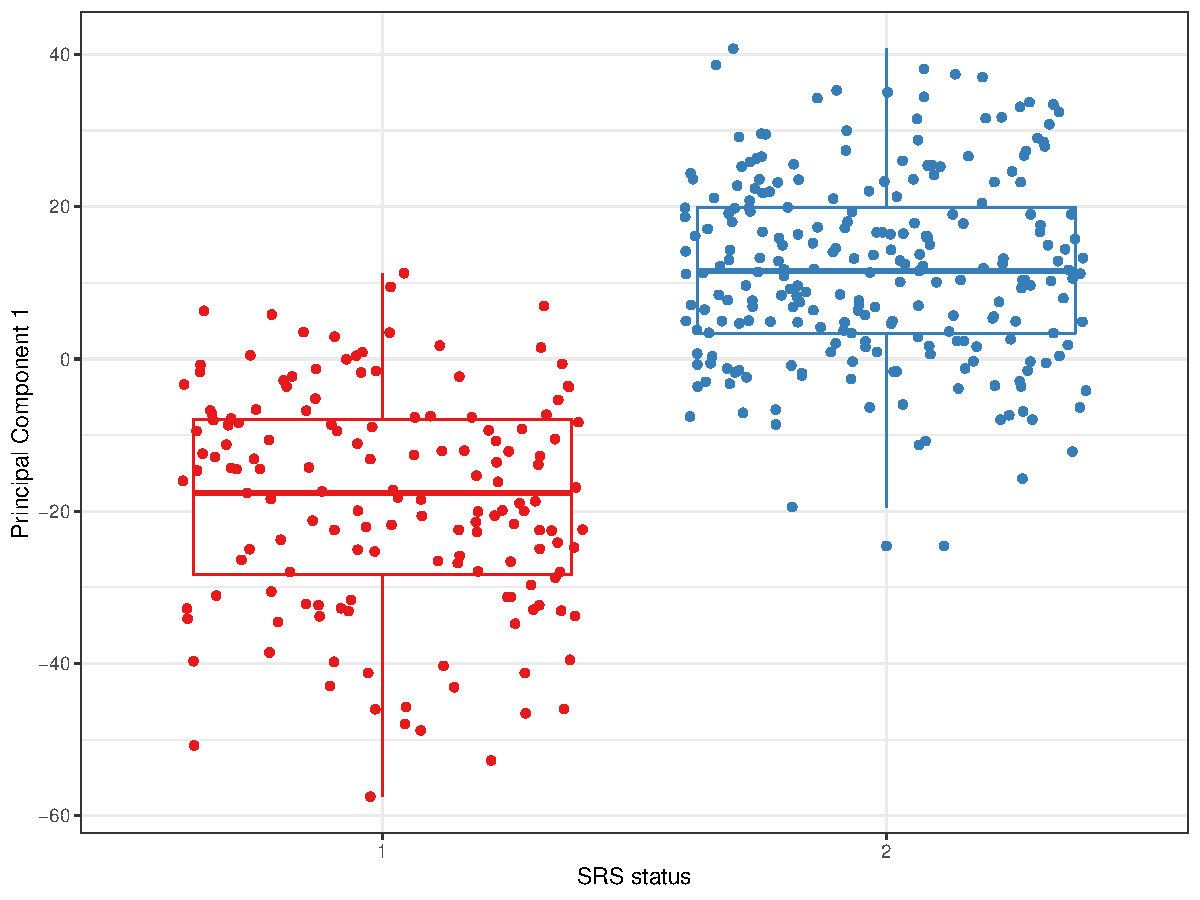
\includegraphics[scale=0.6]{./Results3/Images/PC1.pdf}
\caption[Principal Component 1]{\textbf{Principal Component 1} First principal component (PC1) from principal component analysis of the top 10\% most variable genes expressed by peripheral blood leukocytes, plotted by SRS endotype.}
\label{fig:pc1}
\end{figure}


\begin{figure}[htbp]
\centering
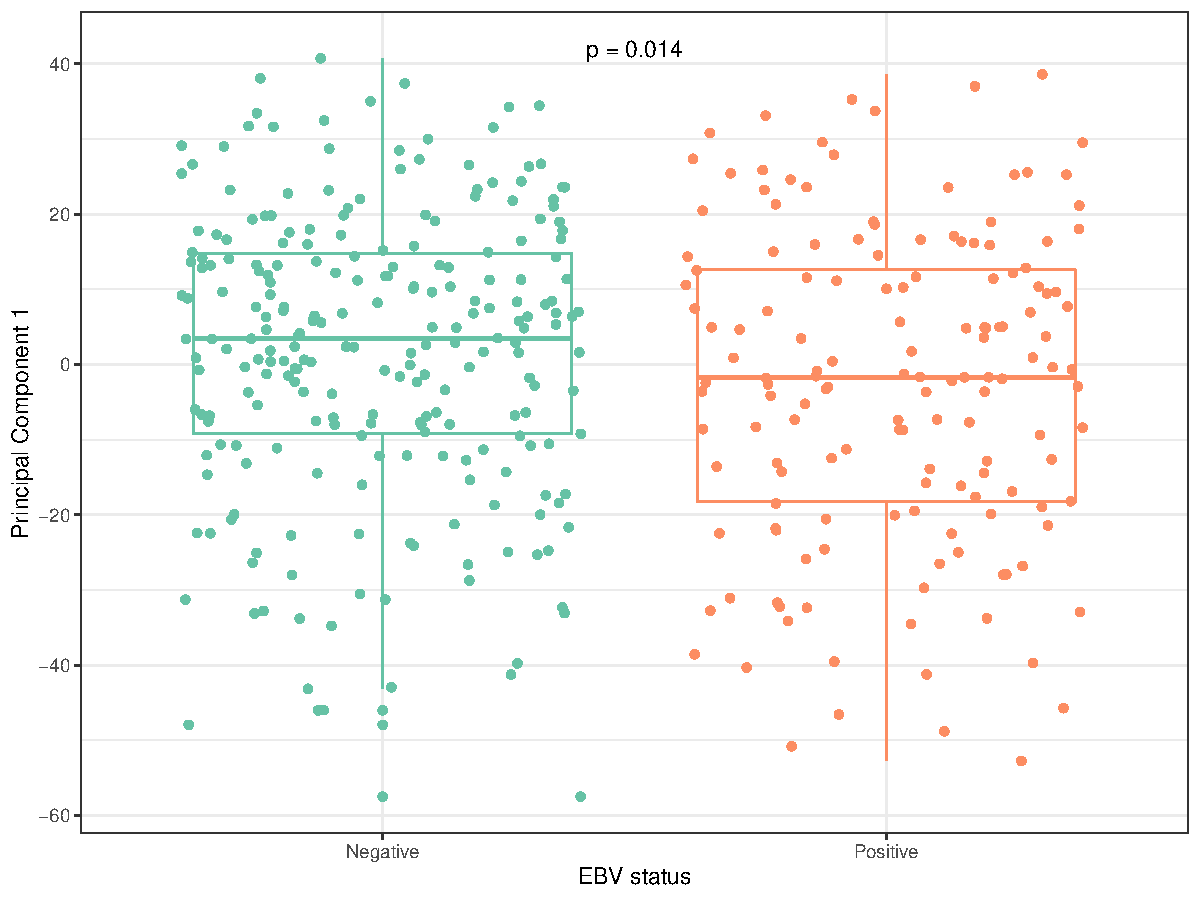
\includegraphics[scale=0.6]{./Results3/Images/SRS_jitter.pdf}
\caption[EBV-positivity and SRS status]{\textbf{Boxplot of first available SRS as a continuous trait against EBV status over the first five days of ICU admission.} The values for principal component 1 (PC1) provide a continuous measure of SRS endotype with higher values representing an SRS2 endotype and lower values representing an SRS1 endotype. }
\label{fig:ebvsrs}
\end{figure}
\FloatBarrier

\textbf{Levels of EBV viraemia.} 
Digital droplet PCR was used to assay EBV in plasma samples (619 samples; 565 patients) over the first five days of admission (days 1,3, and/or 5). The maximum EBV load was related to SRS endotype determined from the first available timepoint after ICU admission (Figure ~\ref{fig:ebvload}). The median EBV load was higher in the SRS1 compared to the SRS2 endotype patients (211 vs 106 copies/ml; p=0.025; Mann-Whitney U-Test). Thus, among those in whom the virus was detected, the two SRS endotypes differed in the amount of EBV measured.

\FloatBarrier
\begin{figure}[htbp]
\centering
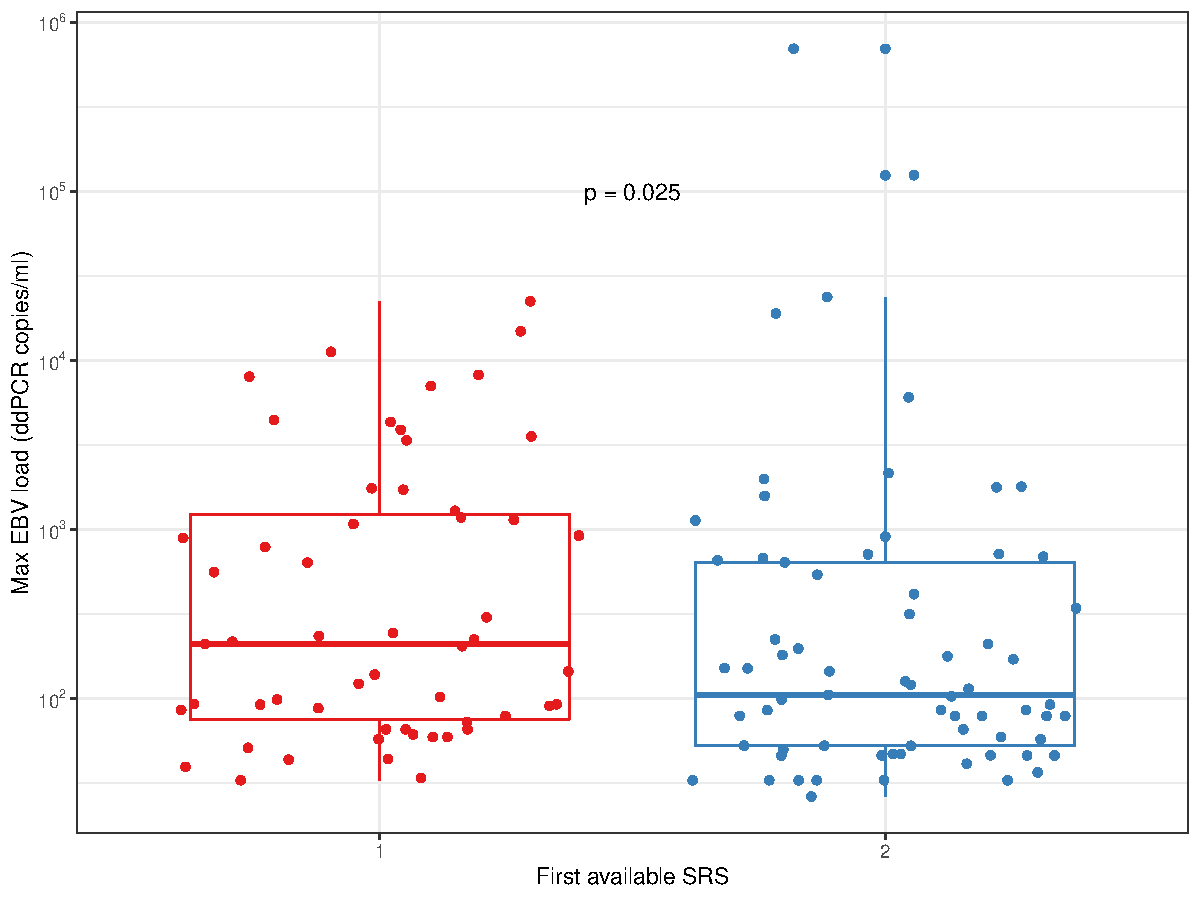
\includegraphics[width=\textwidth]{./Results3/Images/ebvload.pdf}
\caption[EBV load and SRS status]{\textbf{Boxplot of maximum EBV load over the first 5 days of ICU admission (ddPCR) against first available SRS status after ICU admission.} SRS=Sepsis Response Signature. ddPCR=digital droplet PCR}
\label{fig:ebvload}


\end{figure}
\FloatBarrier

\textbf{Gene expression signature.} 
Global gene expression from the peripheral blood total leukocyte population was compared between EBV-positive and EBV-negative individuals (Figure ~\ref{fig:ebvsig1}). The differential expression analysis included only gene expression from patient samples at the first available time point; 28228 probes were tested. Nine genes were differentially expressed at a fold-change $>$1.5 and FDR $<$0.05 (Table ~\ref{tab:ebv-de-genes}). These include \textit{CACNA2D3} (FDR 0.00521, fold change 1.55, downregulated in EBV-positive patients) which is a tumour suppressor gene downregulated in primary nasopharyngeal cancer and nasopharyngeal cell lines compared with non-tumorigenic cells \parencite{Wong2013} and \textit{KIAA0101} (FDR 0.0128, fold change 1.51, upregulated in EBV-positive patients), an Epstein Barr Virus Nuclear Antigen 1 target gene \parencite{Satoh2013}.

Since SRS status is associated with EBV status and is therefore a confounding factor, we repeated the differential expression analysis, this time including SRS as a covariate in the linear model (Figure ~\ref{fig:ebvsig2}). Twelve genes (Table ~\ref{tab:ebv-de-genes-srs}) were found to be differentially expressed; there was an overlap of seven genes with the previous analysis.

Of the seven overlapping genes, there were several with a known role in EBV pathophysiology. These include \textit{CDC20} (FDR 0.00451, fold change 1.53, upregulated in EBV-positive patients) which binds to EBV encoded proteins, activating the mitotic checkpoint and facilitating lytic EBV replication \parencite{Li2015} and \textit{PRTN3} (FDR 0.0468, fold change 1.59, upregulated in EBV-positive patients) which has been observed to be co-expressed with the basigin gene, overexpressed in nasopharyngeal cancer \parencite{Gao2017}.

\FloatBarrier
\begin{figure}[htbp]
\centering
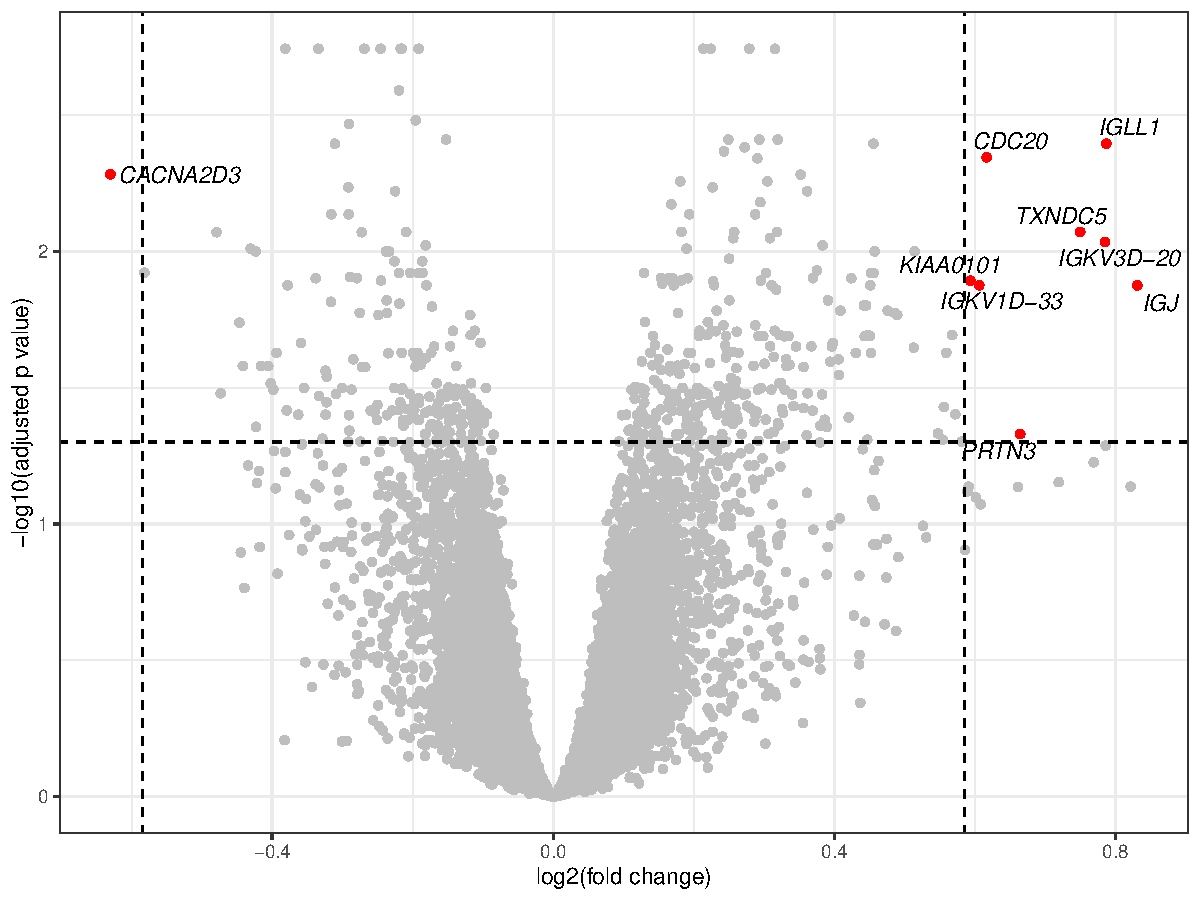
\includegraphics[width=\textwidth]{./Results3/Images/ebvsig1.pdf}
\caption[EBV signature]{\textbf{Volcano plot showing differentially expressed probes between EBV-positive and EBV-negative individuals.} Probes in red (labelled) are differentially expressed at a fold-change of 1.5 and p-value of 0.05. Positive fold change corresponds to upregulation in Epstein-Barr Virus-positive individuals.}
\label{fig:ebvsig1}


\end{figure}

\begin{figure}[htbp]
\centering
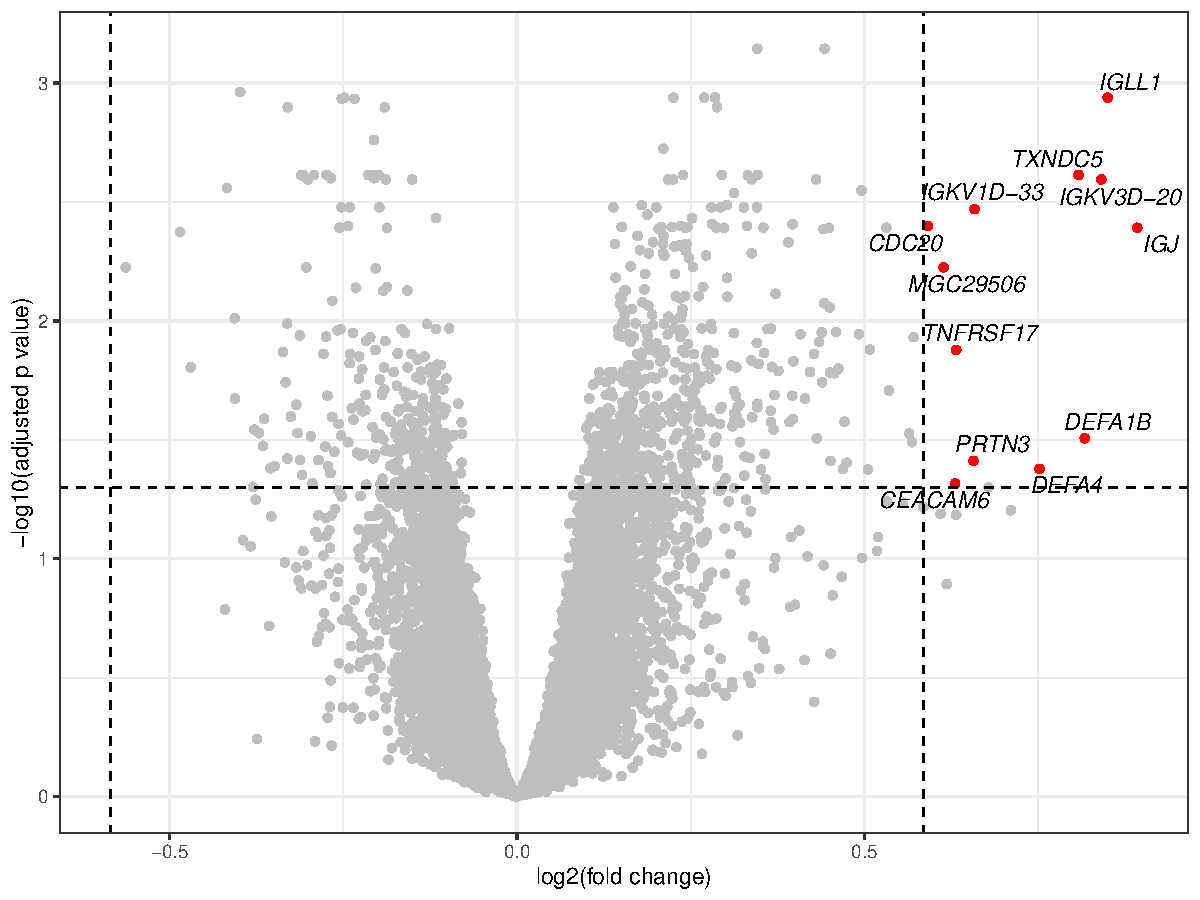
\includegraphics[width=\textwidth]{./Results3/Images/ebvsig2.pdf}
\caption[EBV signature with SRS as covariate]{\textbf{Volcano plot showing differentially expressed probes between EBV-positive and EBV-negative individuals with SRS included in the linear model.} Probes in red (labelled) are differentially expressed at a fold-change of 1.5 and p-value of 0.05. Positive fold change corresponds to upregulation in Epstein-Barr Virus-positive individuals.}
\label{fig:ebvsig2}


\end{figure}
\FloatBarrier

\subsection{Evidence for immunosuppression: \textit{Streptococcus pneumoniae}}

Of the 573 individuals in the metagenomic cohort, 109 had evidence of \textit{Streptococcus pneumoniae} infection. This was comprised of diagnoses made by clinical microbiology (n=92) and new diagnoses made by \textit{Castanet} (n=17). \textit{S. pneumoniae} ddPCR data was available on 99/109 individuals. Of these 99 individuals, 38 were ddPCR positive for \textit{S. pneumoniae}. Clinical characteristics were compared between the ddPCR positive (n=38) and ddPCR negative (n=61) groups (Table ~\ref{tab:strepclin}). 

\FloatBarrier
\begin{table}[]
\begin{center}
\begin{tabular}{|l|l|l|l|}
\hline
\textbf{Characteristic}                                               & \textbf{\begin{tabular}[c]{@{}l@{}}ddPCR-negative\\ (n=61)\end{tabular}} & \textbf{\begin{tabular}[c]{@{}l@{}}ddPCR-positive\\ (n=38)\end{tabular}} & \textbf{p-value} \\ \hline
Age                                                                   & 58.1 (19-84)                                                             & 57.8 (18-89)                                                             & 0.94             \\ \hline
Male sex\textasciicircum{}                                            & 33 (54\%)                                                                & 14 (37\%)                                                                & 0.14             \\ \hline
SRS1\textasciicircum{}                                                & 15/27 (56\%)                                                             & 12/21 (57\%)                                                             & 1.00             \\ \hline
\begin{tabular}[c]{@{}l@{}}Charlson comorbidity\\ index*\end{tabular} & 1.11                                                                     & 0.6                                                                      & 0.028            \\ \hline
Mortality (28-day)`                                                   & 12 (20\%)                                                                & 6 (16\%)                                                                 & 0.6              \\ \hline
ICU length of stay`                                                   & 10.7                                                                     & 13.2                                                                     & 0.3              \\ \hline
SOFA score (day 1)*                                                   & 7.0                                                                      & 7.2                                                                      & 0.39             \\ \hline
SOFA score (maximum)*                                                 & 8.0                                                                      & 8.1                                                                      & 0.42             \\ \hline
Mechanical ventilation\textasciicircum{}                              & 13 (21\%)                                                                & 3 (7.9\%)                                                                & 0.14             \\ \hline
Vasopressors\textasciicircum{}                                        & 20 (33\%)                                                                & 10 (26\%)                                                                & 0.65             \\ \hline
\end{tabular}
\end{center}
\smallskip
\caption[\textit{S. pneumoniae} positivity and clinical outcomes]{\textbf{Clinical characteristics and outcome data compared between ddPCR \textit{S. pneumoniae}-negative and \textit{S. pneumoniae}-positive individuals.} ICU length of stay analysis only includes patients surviving to ICU discharge. T-test performed except where indicated (\textasciicircum{}Chi-squared test; *Mann-Whitney U-test; `Log-rank test). SRS=Sepsis Response Signature; SOFA=Sequential Organ Failure Assessment} 
\label{tab:strepclin}
\end{table}
\FloatBarrier

There was no difference in outcome status of both groups in terms of 28-day mortality, ICU length of stay, SOFA score, mechanical ventilation and vasopressor use. Interestingly however, there was a difference in the Charlson comorbidity index between the two groups with \textit{S. pneumoniae} positive patients showing lower levels of premorbid disease. 

In addition, individuals with a high \textit{S. pneumoniae} bacterial load ($\geq$10$^3$ copies/ml) were compared with individuals with a bacterial load below this threshold (Table ~\ref{tab:strephighclin}). There was no difference in the key outcomes of 28-day mortality, mechanical ventilation and vasopressor use.

\FloatBarrier
\begin{table}[]
\begin{center}
\begin{tabular}{|l|l|l|l|}
\hline
\textbf{Characteristic}                  & \textbf{\begin{tabular}[c]{@{}l@{}}Low/negative \\ \textit{S. pneumoniae}\\ load (n=89)\end{tabular}} & \textbf{\begin{tabular}[c]{@{}l@{}}High \\ \textit{S. pneumoniae}\\ load (n=10)\end{tabular}} & \textbf{p-value} \\ \hline
Mortality (28-day)`                      & 15 (16.9\%)                                                                                  & 3 (30\%)                                                                             & 0.3              \\ \hline
Mechanical ventilation\textasciicircum{} & 0 (0\%)                                                                                      & 10 (100\%)                                                                           & 0.31             \\ \hline
Vasopressors\textasciicircum{}           & 62 (70\%)                                                                                    & 7 (70\%)                                                                             & 1                \\ \hline
\end{tabular}
\end{center}
\caption[High \textit{S. pneumoniae} load and clinical outcomes]{\textbf{Clinical characteristics and outcome data compared between ddPCR \textit{S. pneumoniae}-low/negative and ddPCR \textit{S. pneumoniae}-high individuals.} Individuals with a bacterial load of $\geq$10$^3$ were classified as having a high \textit{S. pneumoniae} bacterial load. (\textasciicircum{}Chi-squared test; `Log-rank test). } 
\label{tab:strephighclin}
\end{table}

Given the findings with EBV, it was possible that levels of \textit{Streptococcus pneumoniae} bacteraemia might also differ between the two SRS1 endotypes. For patients with \textit{S. pneumoniae} infection diagnosed by clinical microbiology (n=92), ddPCR was used to assay \textit{S. pneumoniae} in plasma samples over the first five days of admission (days 1,3, and/or 5) and the earliest value noted. For individuals with detectable bacterial load in plasma, this was evaluated against SRS endotype from the same day where expression data was available (n=18) (Figure ~\ref{fig:strepsrs}). There was a statistically significant difference between the two groups, with SRS1 endotype patients showing a higher median \textit{S. pneumoniae} load compared to SRS2 endotype patients (12293 vs 234 copies/ml; p=0.0022; Mann-Whitney U Test).

\FloatBarrier
\begin{figure}[htbp]
\centering
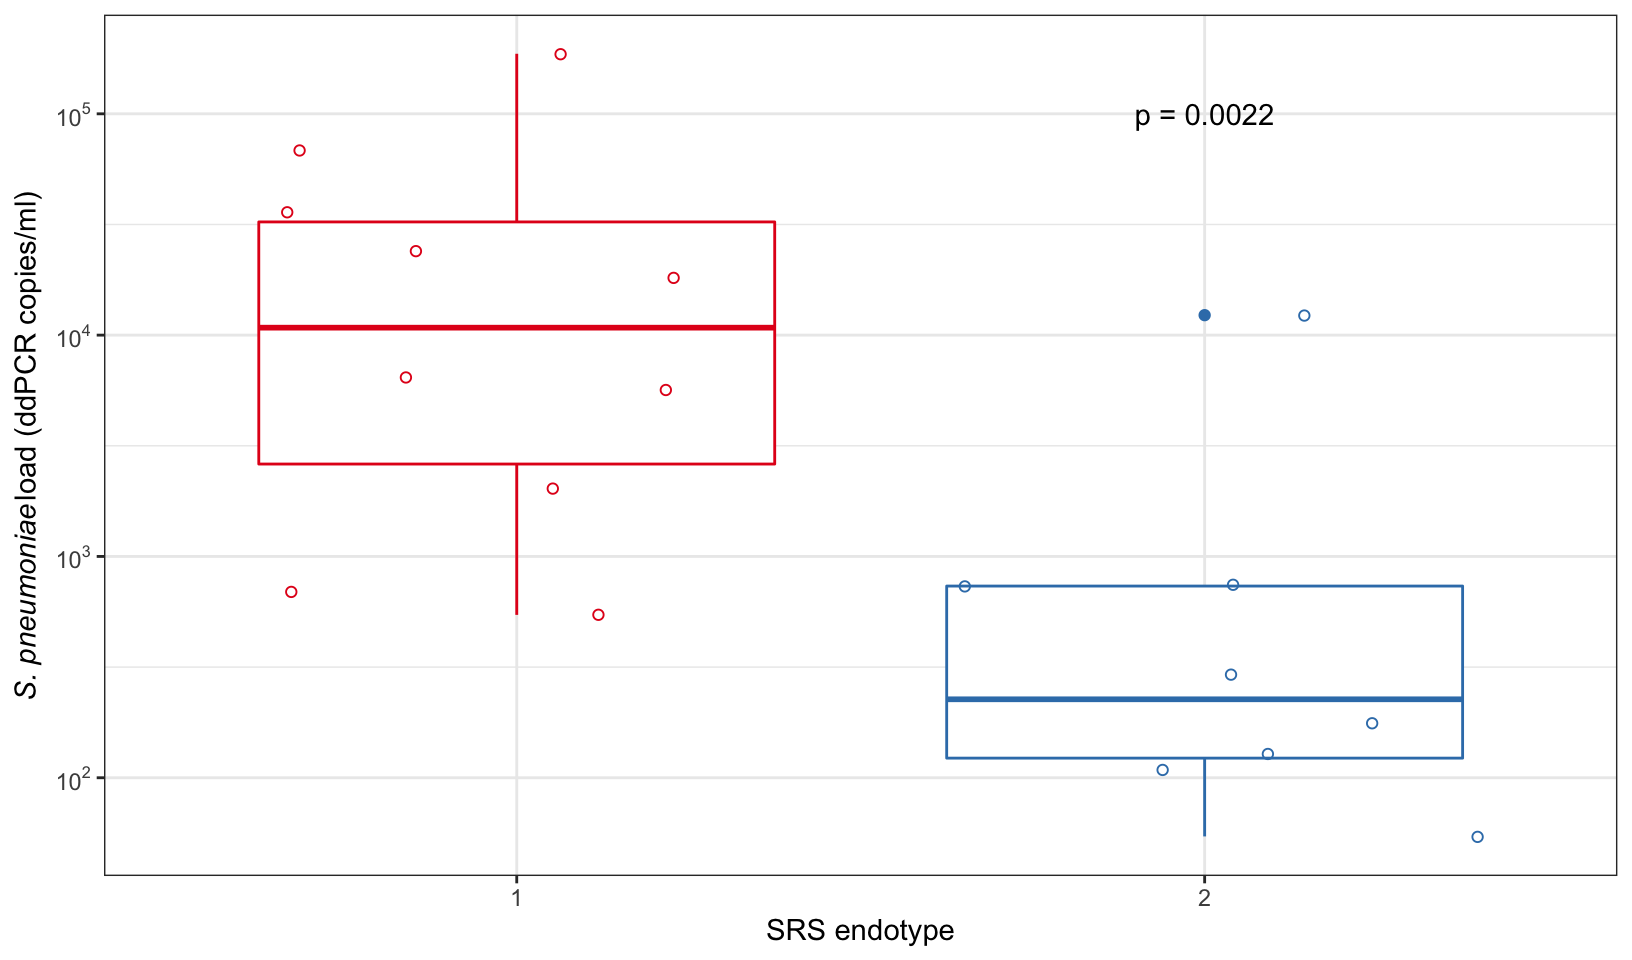
\includegraphics[width=\textwidth]{./Results3/Images/strepsrs.png}
\caption[\textit{S. pneumoniae} load and SRS status]{\textbf{Boxplot of \textit{Streptococcus pneumoniae} load and SRS status.} SRS=Sepsis Response Signature}
\label{fig:strepsrs}


\end{figure}
\FloatBarrier

\subsection{Transcriptomic signature of viral infection}
Of the 408 CAP patients with expression data following QC, there were 166 individuals with a diagnosis of either bacterial (n=136) or viral (n=30) infection. Microbiological phenotyping was based on clinical information from the eCRF and metagenomic data. Individuals with a mixed bacterial/viral infection, fungal infection or no positive microbiology were excluded from the comparison since they could not be accurately allocated to either the bacterial or viral category.

\textbf{Clinical characteristics and outcome.} Table \ref{tab:viralclinical} details the clinical characteristics and outcome data for the bacterial and viral groups. There was no significant difference in age, sex, baseline comorbidities, mortality, length of stay or SOFA score between the two groups. However, there were significantly more patients with an SRS2 endotype in the viral group compared with the bacterial group. PC1 was plotted against infection type (Figure \ref{fig:viralsrs2}), showing that patients with bacterial infection were evenly distributed across the spectrum of SRS1/SRS2 whilst patients with viral infection displayed a more SRS2-like endotype.

\begin{table}[]
\begin{center}
\begin{tabular}{|l|l|l|l|}
\hline
\textbf{Characteristic}    & \textbf{\begin{tabular}[c]{@{}l@{}}Viral\\ (n=30)\end{tabular}} & \textbf{\begin{tabular}[c]{@{}l@{}}Bacterial \\ (n=136)\end{tabular}} & \textbf{p-value} \\ \hline
Age                        & 57.8 (25-83)                                                    & 63.0 (18-92)                                                          & 0.11             \\ \hline
Male sex\textasciicircum{}                   & 14 (47\%)                                                       & 78 (57\%)                                                             & 0.29             \\ \hline
SRS1\textasciicircum{}                       & 9 (30\%)                                                        & 72 (53\%)                                                             & 0.038            \\ \hline
Charlson comorbidity index* & 0.8                                                             & 1.1                                                                   & 0.52             \\ \hline
Mortality (28-day)`         & 9 (30\%)                                                        & 38 (28\%)                                                             & 0.3              \\ \hline
ICU length of stay`         & 17.7                                                            & 13.4                                                                  & 0.3              \\ \hline
SOFA score (day 1)*       & 6.1                                                             & 7.1                                                                   & 0.12             \\ \hline
SOFA score (maximum)*       & 7.3                                                             & 8.2                                                                   & 0.33             \\ \hline
\end{tabular}
\end{center}
\smallskip
\caption[Viral vs bacterial infection]{\textbf{Viral vs bacterial infection: clinical characteristics and outcome data.} ICU length of stay analysis only includes patients surviving to ICU discharge. T-test performed except where indicated (\textasciicircum{}Chi-squared test; *Mann-Whitney U-test; `Log-rank test).}
\label{tab:viralclinical}
\end{table}

\FloatBarrier
\begin{figure}[htbp]
\centering
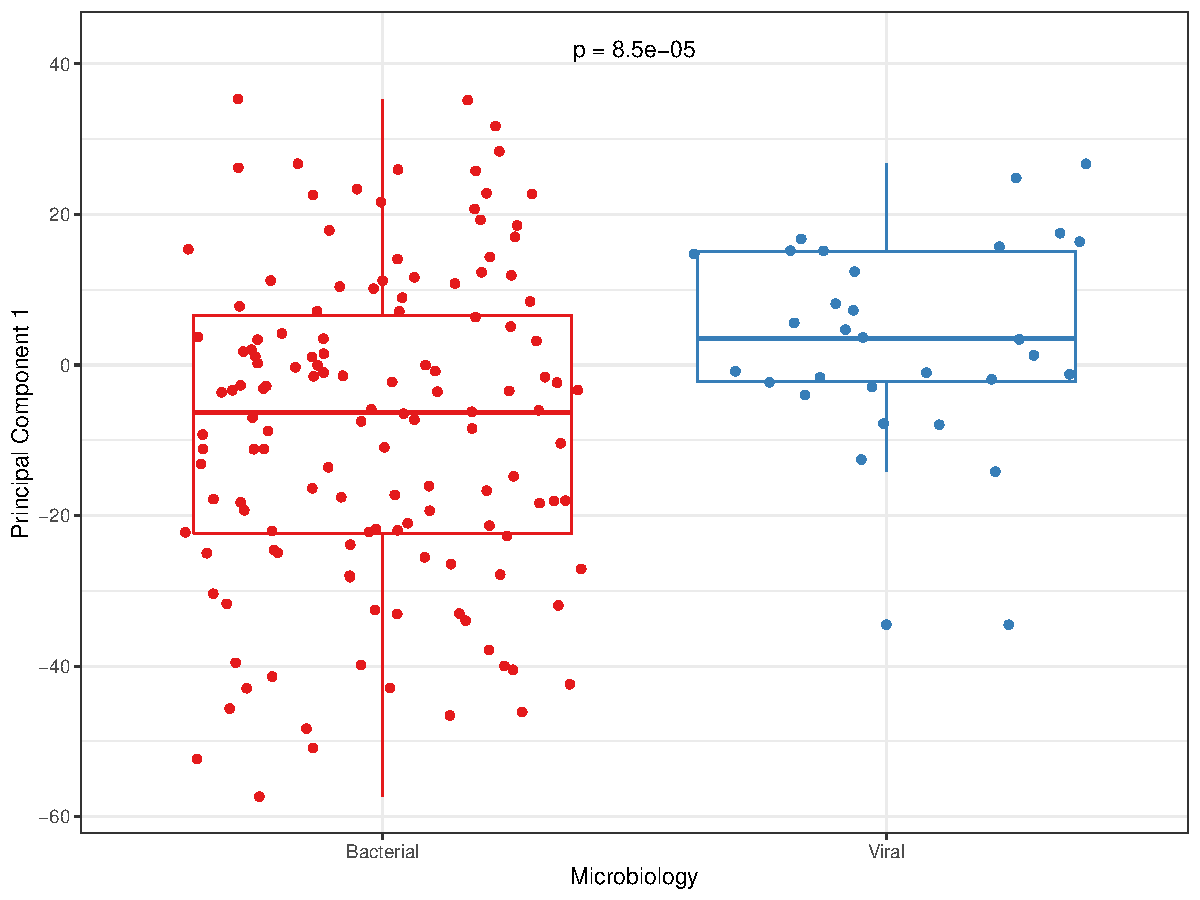
\includegraphics[width=\textwidth]{./Results3/Images/viralSRS2.pdf}
\caption[Microbiology and SRS status]{\textbf{Boxplot of first available SRS as a continuous trait against microbiology.} The values for principal component 1 (PC1) provide a continuous measure of SRS endotype with higher values representing an SRS2 endotype and lower values representing an SRS1 endotype. SRS=Sepsis Response Signature}
\label{fig:viralsrs2}
\end{figure}
\FloatBarrier

\textbf{Differential gene expression.} The gene expression of individuals with viral (n=30) and bacterial (n=136) infection was contrasted. This identified 206 differentially expressed probes (FDR $<$0.05 and fold change $>$1.5) with the majority upregulated in individuals with viral infection (Figure ~\ref{fig:vp-viral-bacterial}) (Table ~\ref{tab:vb-de-genes}). 

\FloatBarrier
\begin{figure}[htbp]
\centering
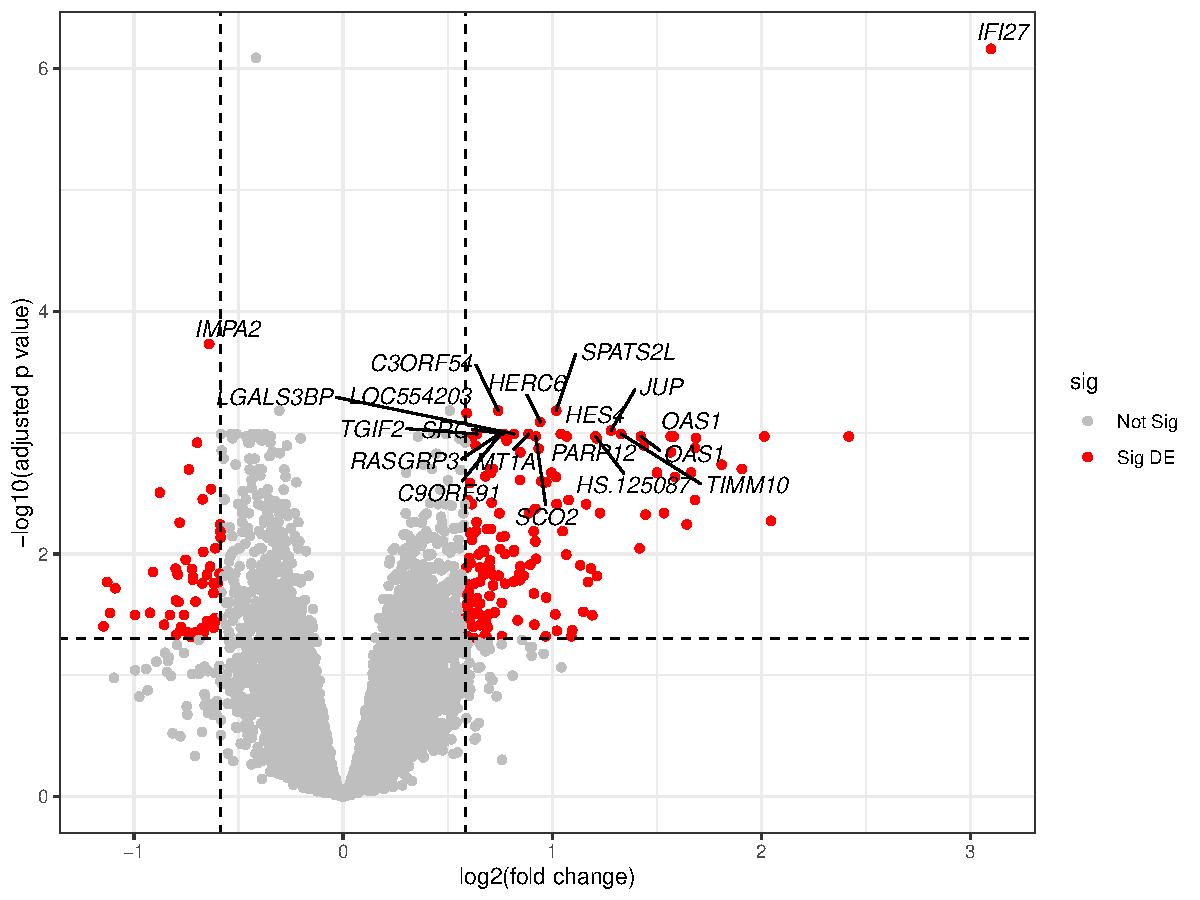
\includegraphics[width=\textwidth]{./Results3/Images/vp-viral-bacterial.pdf}
\caption[Volcano plot of differentially expressed probes in viral infection]{\textbf{Volcano plot of differentially expressed probes in viral vs bacterial infection.} Probes in red are differentially expressed at a FDR $<$0.05 and fold change $>$1.5. Positive fold change corresponds to upregulation in individuals with viral infection. Top 20 significantly differentially expressed probes are labelled.}
\label{fig:vp-viral-bacterial}
\end{figure}
\FloatBarrier

\textbf{Pathway enrichment.} Enrichment analysis was performed on the 206 probes identified as being differentially expressed using the R package XGR \parencite{Fang2016} and the Gene Ontology database \parencite{GO2019} \parencite{Ashburner2000}. A number of pathways specific to the immune response to viral infection were identified (Figure ~\ref{fig:xgr-viral}), including the type 1 interferon signalling pathway and the regulation of viral genome replication.

\FloatBarrier
\begin{figure}[htbp]
\centering
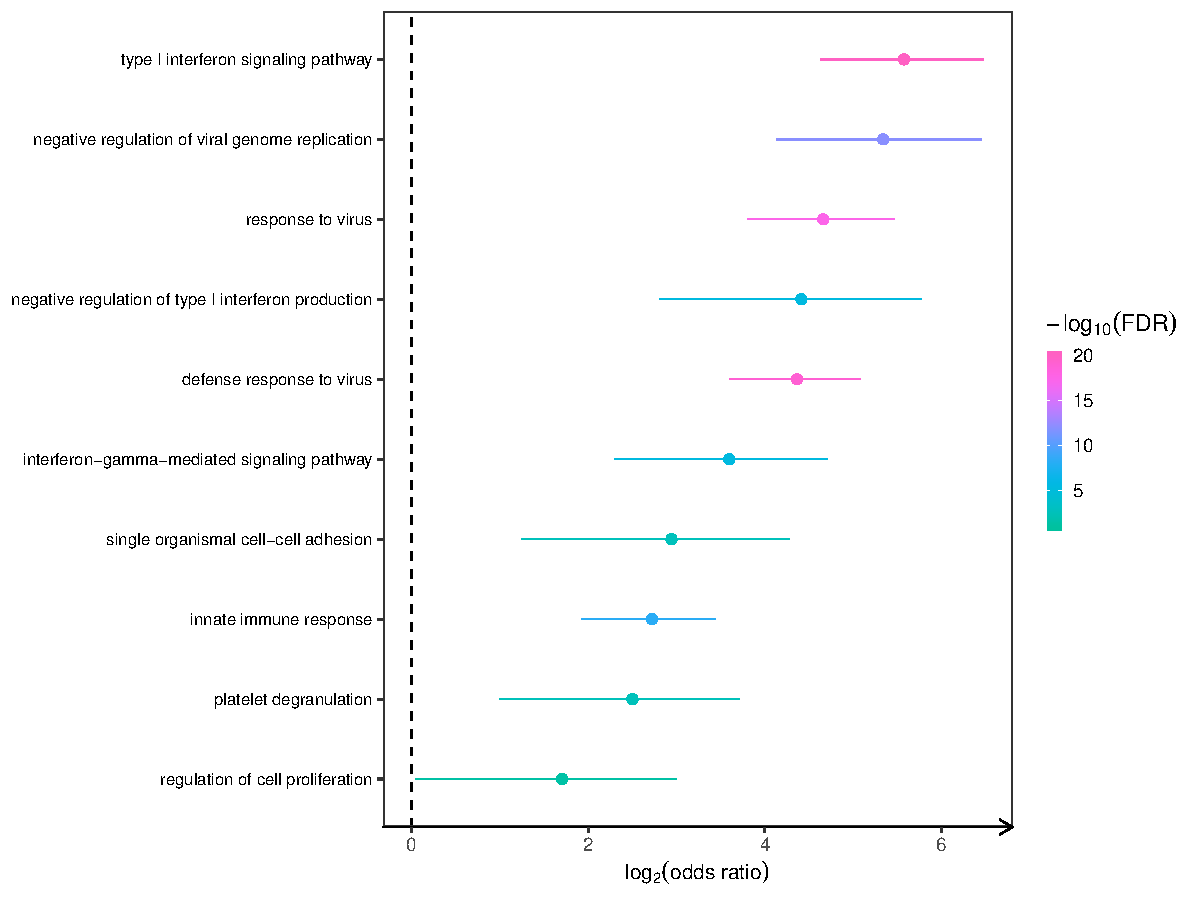
\includegraphics[width=\textwidth]{./Results3/Images/xgr-viral.pdf}
\caption[Pathway analysis for viral infection]{\textbf{Pathway enrichment for viral infection.} The differentially expressed probes between patients with viral and bacterial infection were used to determine pathway enrichment with XGR. The top ten most enriched pathways using the Gene Ontology database are shown.}
\label{fig:xgr-viral}
\end{figure}
\FloatBarrier
 
 \textbf{Predictive gene signature.} Differentiating viral from bacterial CAP remains a challenge in the clinical setting. Therefore, a subset of genes was selected for a prediction model from the 206 probes differentially expressed between individuals with viral and bacterial infection. 
 
The 166 individuals with bacterial (n=136) or viral (n=30) infection formed the training cohort for the model. Logistic regression with variable selection was applied to the 206 differentially expressed probes (FDR $<$0.05, fold change $>$1.5) using the elastic net method \parencite{Zou2005} \parencite{Herberg2016}. This is a variable selection algorithm that is an alternative to standard linear regression with least squares fitting, particularly suited to cases where the number of predictors greatly exceeds the number of observations. Elastic net combines the lasso and ridge regression methods of shrinkage, minimising the number of variables included (lasso) whilst also making the model less dependent on any one variable (ridge).
 
Ten probes, corresponding to ten genes were selected by the model: \textit{BTBD11, C3ORF54, IFI27, IMPA2, MT1A, RNASE1, SIGLEC10, SRC, TIMM10, TSPAN13}. In the training dataset, the signature had an AUC of 88.6\% (95\% CI 80.7\%-96.5\%) (Figure ~\ref{fig:roc-vb}). Youden's method was used to select a threshold (0.2017) for discriminating bacterial from viral infection. At this threshold, 114/136 bacterial infections were correctly predicted (specificity 83.8\% [95\% CI 77.2\%-89.7\%]) whilst 25/30 viral infections were correctly predicted (sensitivity 83.3\% [95\% CI 70.0\%-96.7\%]) (Figure ~\ref{fig:boxplot-vb}). This equated to a misclassification rate of 16.3\%.
 
Due to limitations in data availability, it was not possible to select a single validation cohort which included both bacterial and viral infections. Therefore two validation cohorts were used, MOSAIC and VANISH. The Mechanisms of Severe Acute Influenza Consortium (MOSAIC) cohort included 109 adults with confirmed influenza while the Vasopressin vs Norepinephrine as Initial Therapy in Septic Shock (VANISH) cohort included 24 adults with predominantly bacterial sepsis requiring vasopressors. 

For the combined validation cohort, the signature had an AUC of 97.1\% (95\% CI 94.6\%-99.5\%) (Figure ~\ref{fig:roc-vb}). Using the threshold selected for the training cohort, 20/23 bacterial infections were correctly predicted (specificity 87.0\% [95\% CI 73.8\%-100.0\%]) whilst 100/110 viral infections were correctly predicted (sensitivity 90.1\% [95\% CI 85.5\%-96.4\%]) (Figure ~\ref{fig:boxplot-vb}). This equated to a misclassification rate of 9.8\%. 

\FloatBarrier
\begin{figure}[htbp]
\centering
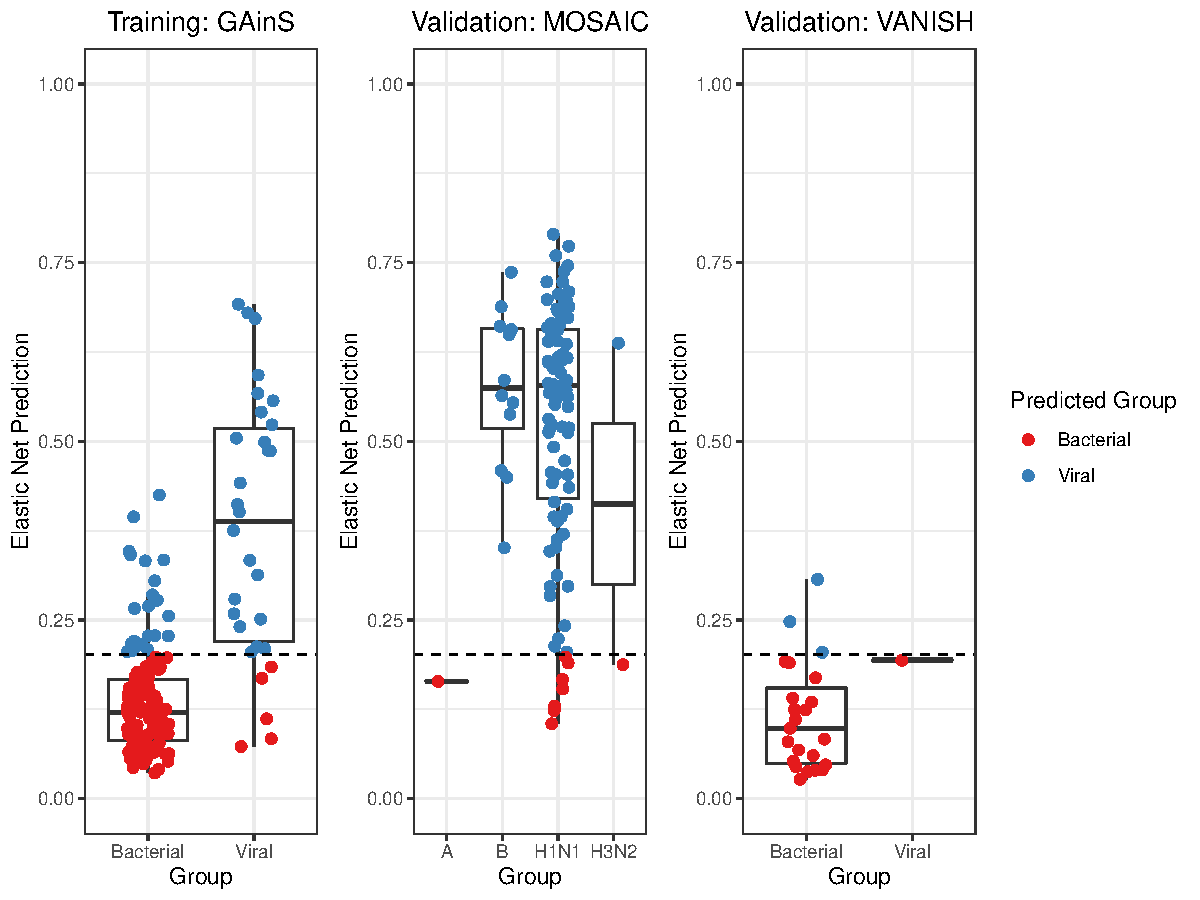
\includegraphics[width=\textwidth]{./Results3/Images/boxplot-viral-signature.pdf}
\caption[Boxplot of viral vs bacterial signature]{\textbf{Boxplot of predictions from viral vs bacterial gene signature.} Each point corresponds to a patient. Actual microbiological groups are plotted on the x-axis whilst predicted classifications are denoted by point colour. The MOSAIC groupings correspond to influenza virus types. Threshold for discriminating bacterial from viral infection is denoted by the dashed line. The elastic net prediction value (y-axis) can range from 0 (indicating bacterial infection) to 1 (indicating viral infection).}
\label{fig:boxplot-vb}
\end{figure}
\FloatBarrier


\FloatBarrier
\begin{figure}[htbp]
\centering
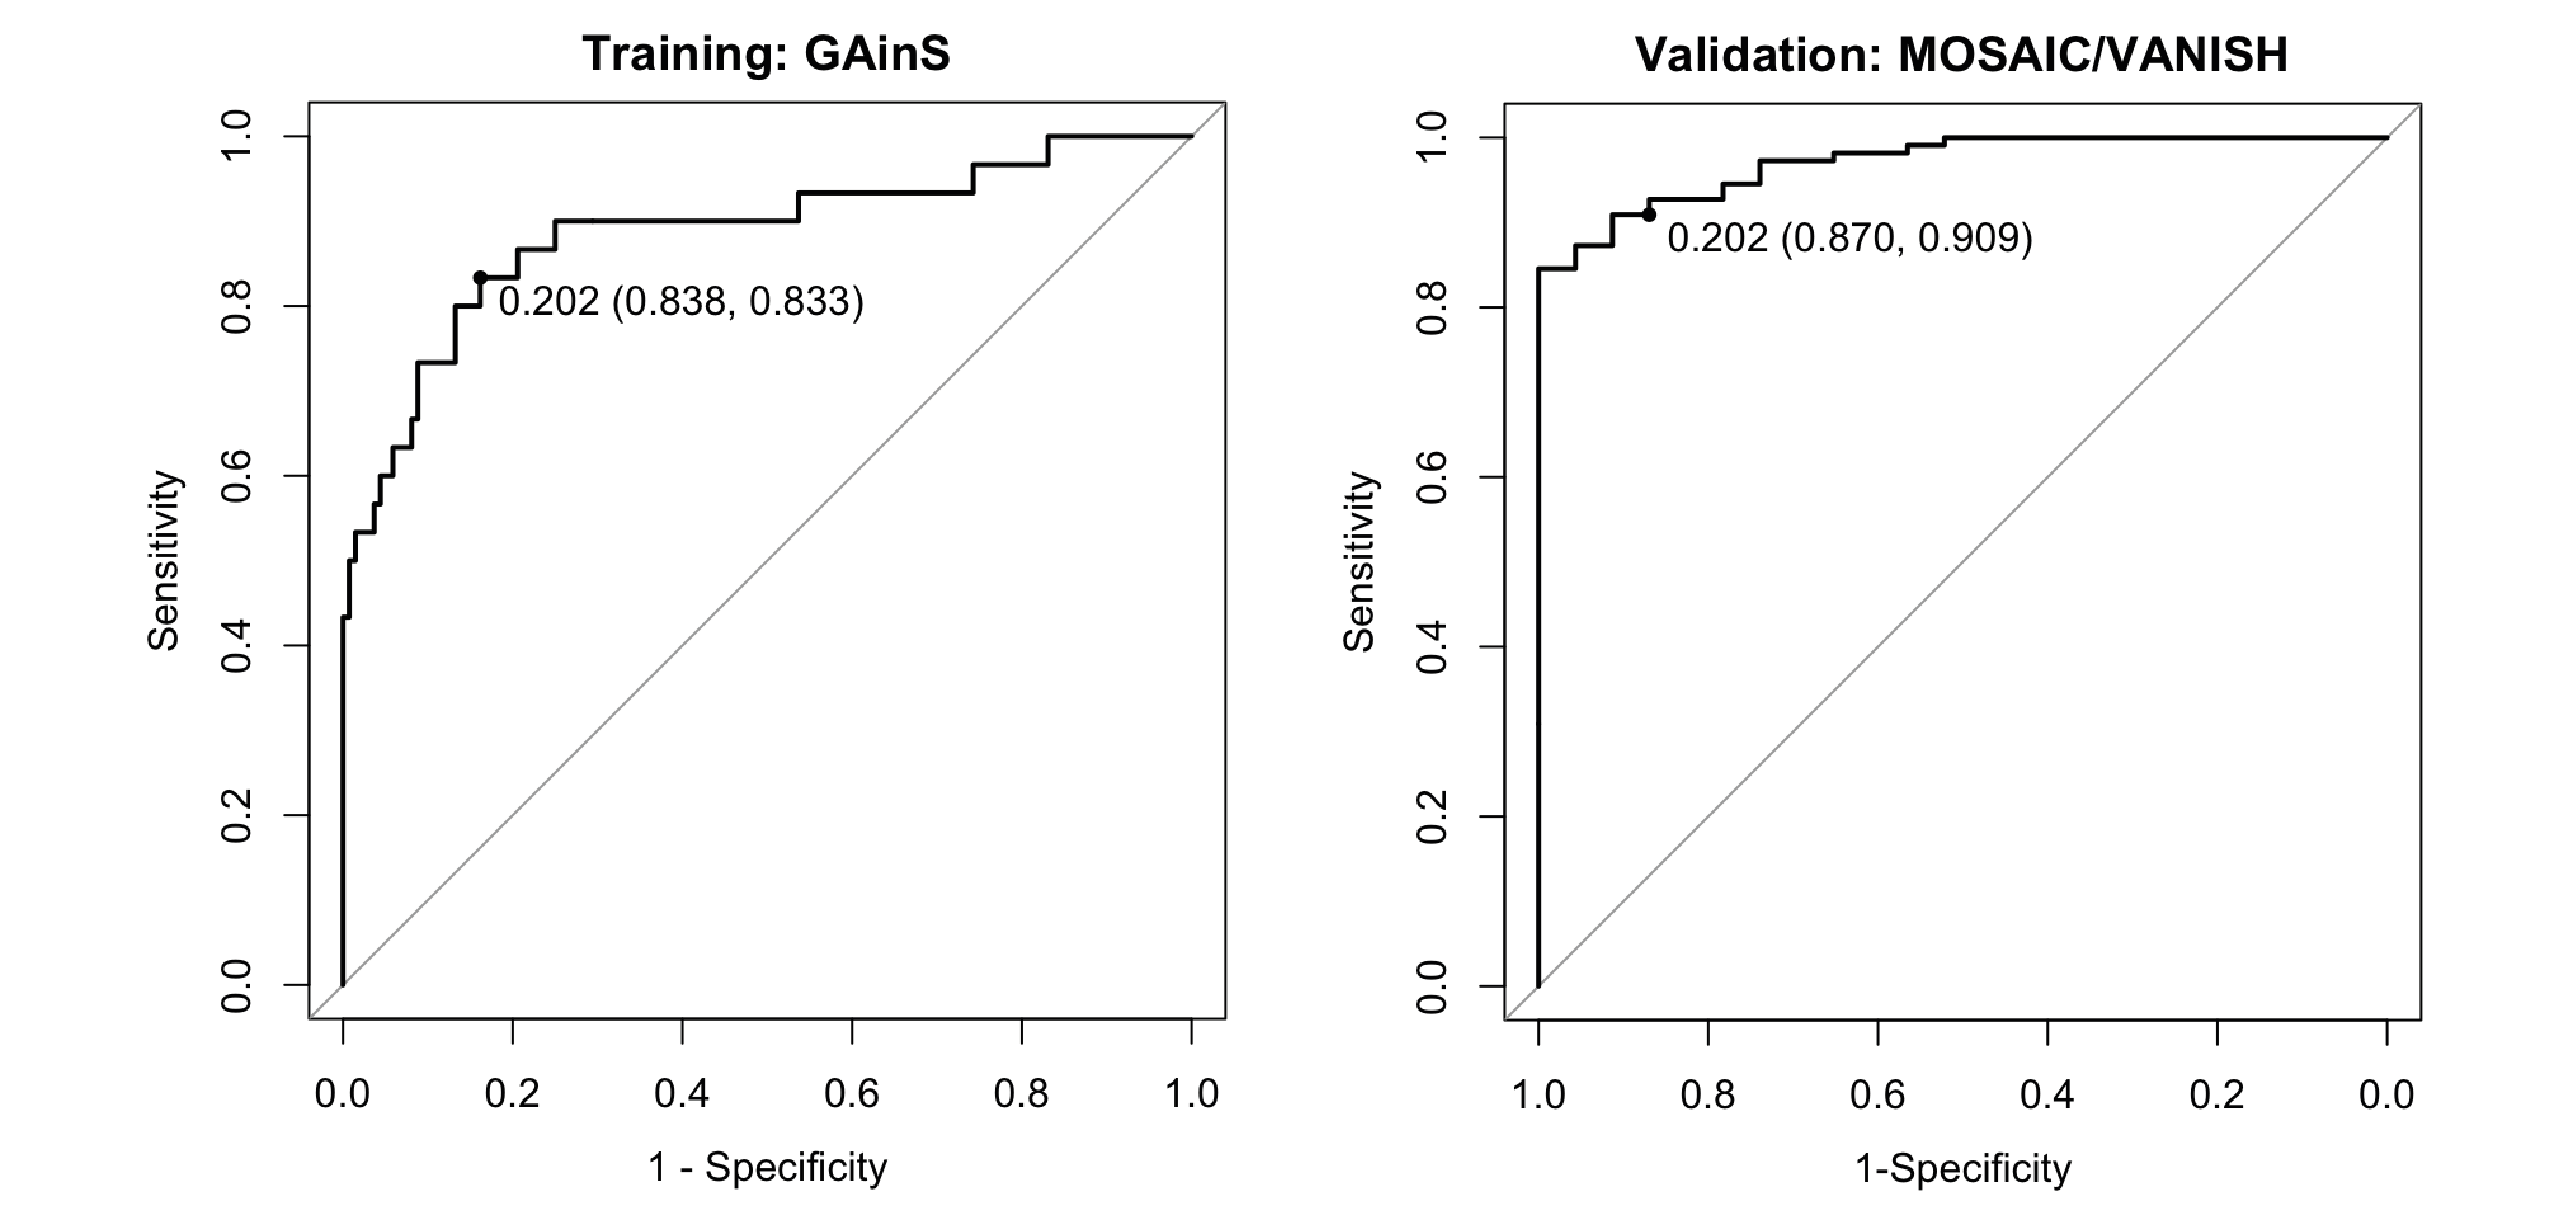
\includegraphics[width=\textwidth]{./Results3/Images/bv-roc-combined.png}
\caption[ROC analysis for viral vs bacterial signature]{\textbf{ROC analysis for viral vs bacterial signature.} The threshold for discriminating bacterial from viral infection is noted (0.202), together with the specificity and sensitivity at that threshold in brackets. AUC for the training cohort was 88.6\% (95\% CI 80.7\%-96.5\%) whilst AUC for the combined validation cohort was 97.1\% (95\% CI 94.6\%-99.5\%). MR was 16.3\% for the training cohort and 9.8\% for the validation cohort.}
\label{fig:roc-vb}
\end{figure}
\FloatBarrier

\subsection{Transcriptomic signature of influenza infection}
\textbf{Differential gene expression.} Two thirds of the viral cohort in the preceding section had influenza infection. The gene expression of these individuals (n=20) was contrasted with that of individuals with bacterial infection (n=136). This identified 139 differentially expressed probes (FDR $<$0.05 and fold change $>$1.2) (Figure ~\ref{fig:vp-flu}) (Table ~\ref{tab:flu-de-genes}).

\FloatBarrier
\begin{figure}[htbp]
\centering
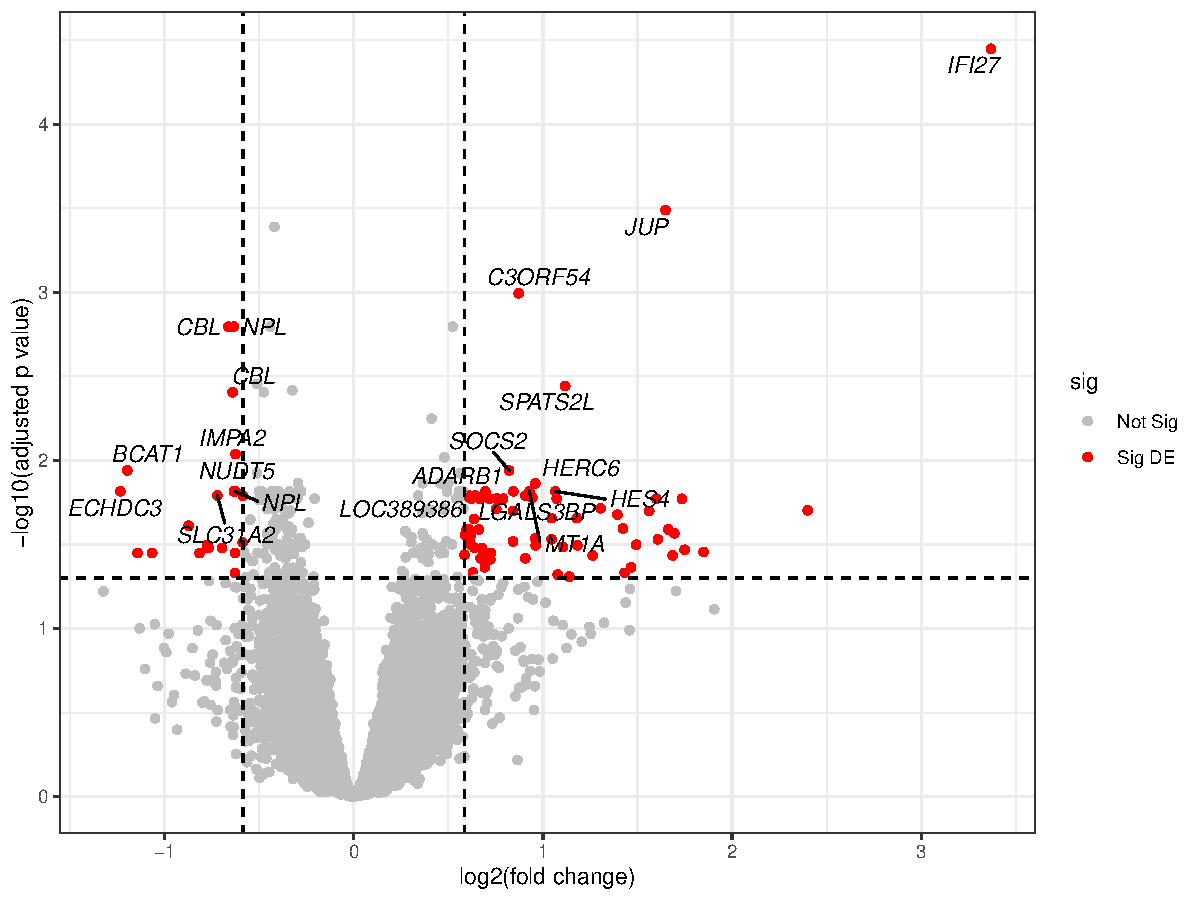
\includegraphics[width=\textwidth]{./Results3/Images/vp-flu.pdf}
\caption[Volcano plot of differentially expressed probes in influenza infection]{\textbf{Volcano plot of differentially expressed probes in influenza vs bacterial infection.} Probes in red are differentially expressed at a FDR $<$0.05 and fold change $>$1.5. Positive fold change corresponds to upregulation in influenza-positive individuals. Top 20 significantly differentially expressed probes are labelled.}
\label{fig:vp-flu}
\end{figure}
\FloatBarrier

\textbf{Pathway enrichment.} Enrichment analysis was performed on the 139 probes identified as being differentially expressed using the R package XGR \parencite{Fang2016} and the Gene Ontology database \parencite{GO2019} \parencite{Ashburner2000}. Similar pathways identified in the viral vs bacterial analysis were identified again here (Figure ~\ref{fig:xgr-flu}), including the type 1 interferon signalling pathway, the regulation of viral genome replication, and viral response.

\FloatBarrier
\begin{figure}[htbp]
\centering
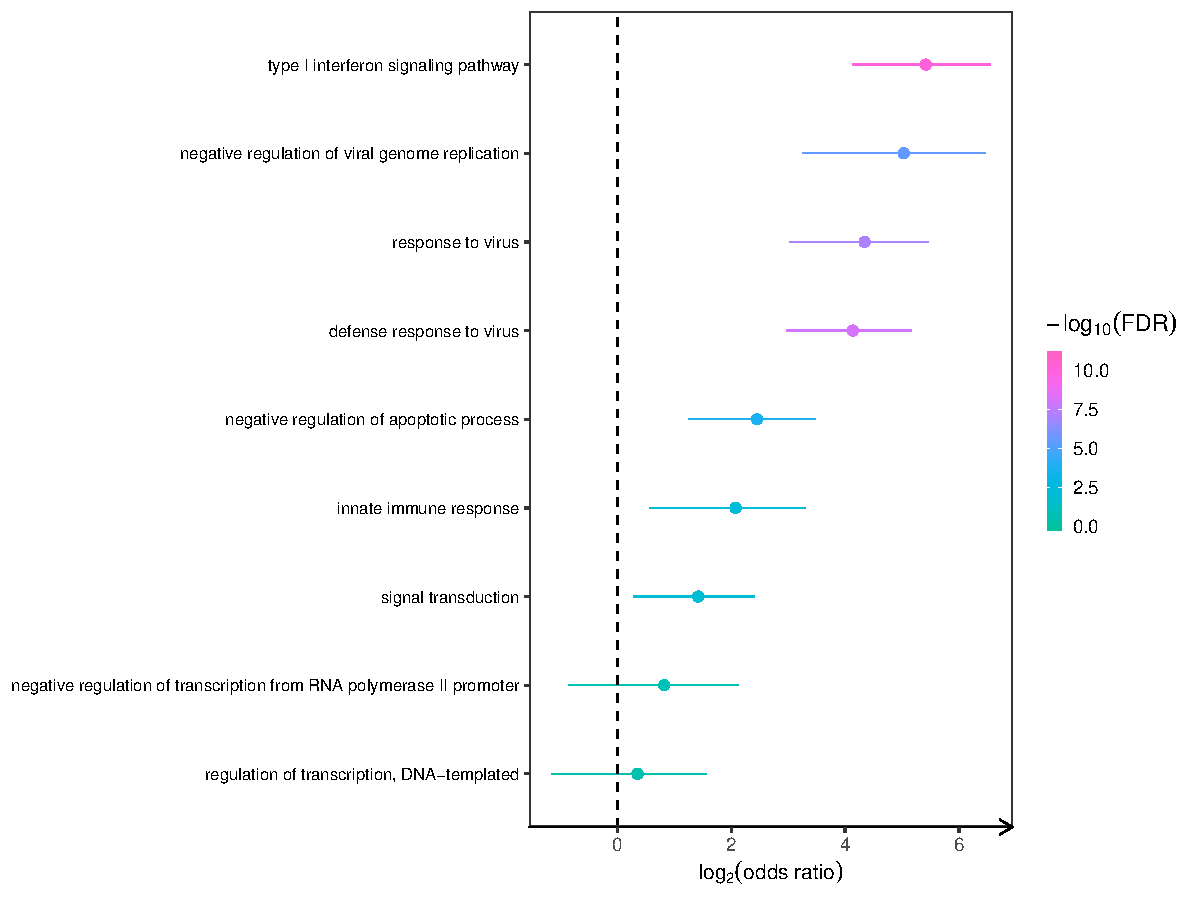
\includegraphics[width=\textwidth]{./Results3/Images/xgr-flu.pdf}
\caption[Pathway analysis for influenza infection]{\textbf{Pathway enrichment for influenza infection.} The differentially expressed probes between patients with influenza and bacterial infection were used to determine pathway enrichment with XGR. The top ten most enriched pathways using the Gene Ontology database are shown.}
\label{fig:xgr-flu}
\end{figure}
\FloatBarrier


\textbf{Predictive gene signature.}
The elastic net method was used again here to select a subset of predictive genes from the 139 differentially expressed probes. The training dataset comprised 156 individuals from the GAinS cohort, 20 with influenza infection and 136 with bacterial infection. 

Seven probes corresponding to seven genes were selected by the elastic net model: \textit{IFI27, JUP, C3ORF54, NPL, CBL, UBQLNL, LOC401845}. In the training dataset, the signature had an AUC of 90.1\% (95\% CI 80.4\%-99.8\%) (Figure ~\ref{fig:roc-flu}). Youden's method was used to select a threshold (0.182) for discriminating bacterial from influenza infection. At this threshold, 123/136 bacterial infections were correctly predicted (specificity 90.4\% [95\% CI 85.3\%-94.9\%]) whilst 16/20 viral infections were correctly predicted (sensitivity 80\% [95\% CI 60\%-95\%]) (Figure ~\ref{fig:boxplot-flu}). This equated to a misclassification rate of 10.9\%.

The two validation cohorts (MOSAIC and VANISH) were used again here with the MOSAIC cohort comprising 109 individuals with influenza infection and the VANISH cohort comprising 23 patients with bacterial sepsis and 1 patient with influenza sepsis.

For the combined validation cohort, the signature had an AUC of 92.9\% (95\% CI 88.5\%-97.4\%) (Figure ~\ref{fig:roc-flu}). Using the threshold identified in the training cohort, 20/23 bacterial infections were correctly predicted (specificity 87\% [95\% CI 73.9\%-100\%]) whilst 89/110 viral infections were correctly predicted (sensitivity 80.9\% [95\% CI 73.6\%-88.2\%]) (Figure ~\ref{fig:boxplot-flu}). This equated to a misclassification rate of 18\%. 

\FloatBarrier
\begin{figure}[htbp]
\centering
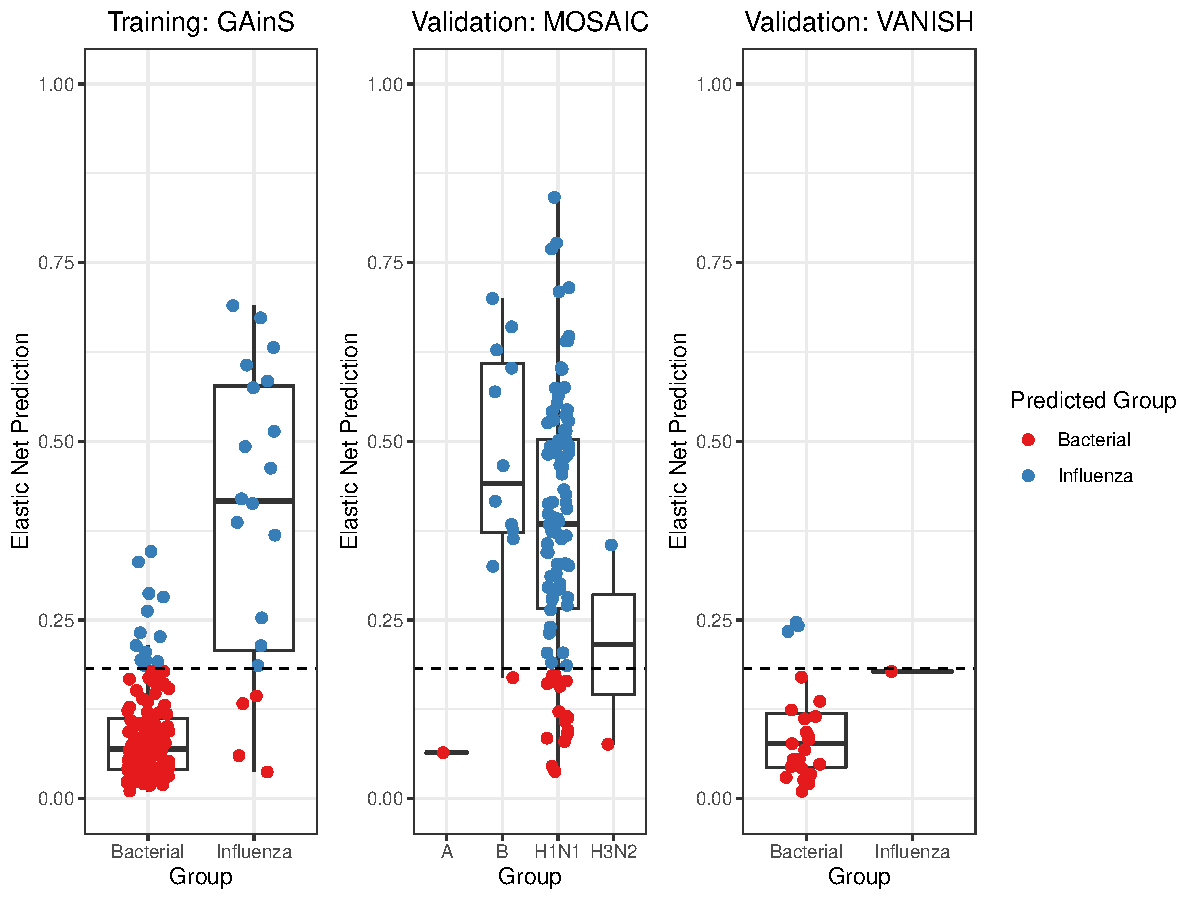
\includegraphics[width=\textwidth]{./Results3/Images/boxplot-influenza-signature.pdf}
\caption[Boxplot of influenza vs bacterial signature]{\textbf{Boxplot of predictions from influenza vs bacterial gene signature.} Each point corresponds to a patient. Actual microbiological groups are plotted on the x-axis whilst predicted classifications are denoted by point colour. The MOSAIC groupings correspond to influenza virus types. Threshold for discriminating bacterial from influenza infection is denoted by the dashed line. The elastic net prediction value (y-axis) can range from 0 (indicating bacterial infection) to 1 (indicating influenza infection).}
\label{fig:boxplot-flu}
\end{figure}
\FloatBarrier


\FloatBarrier
\begin{figure}[htbp]
\centering
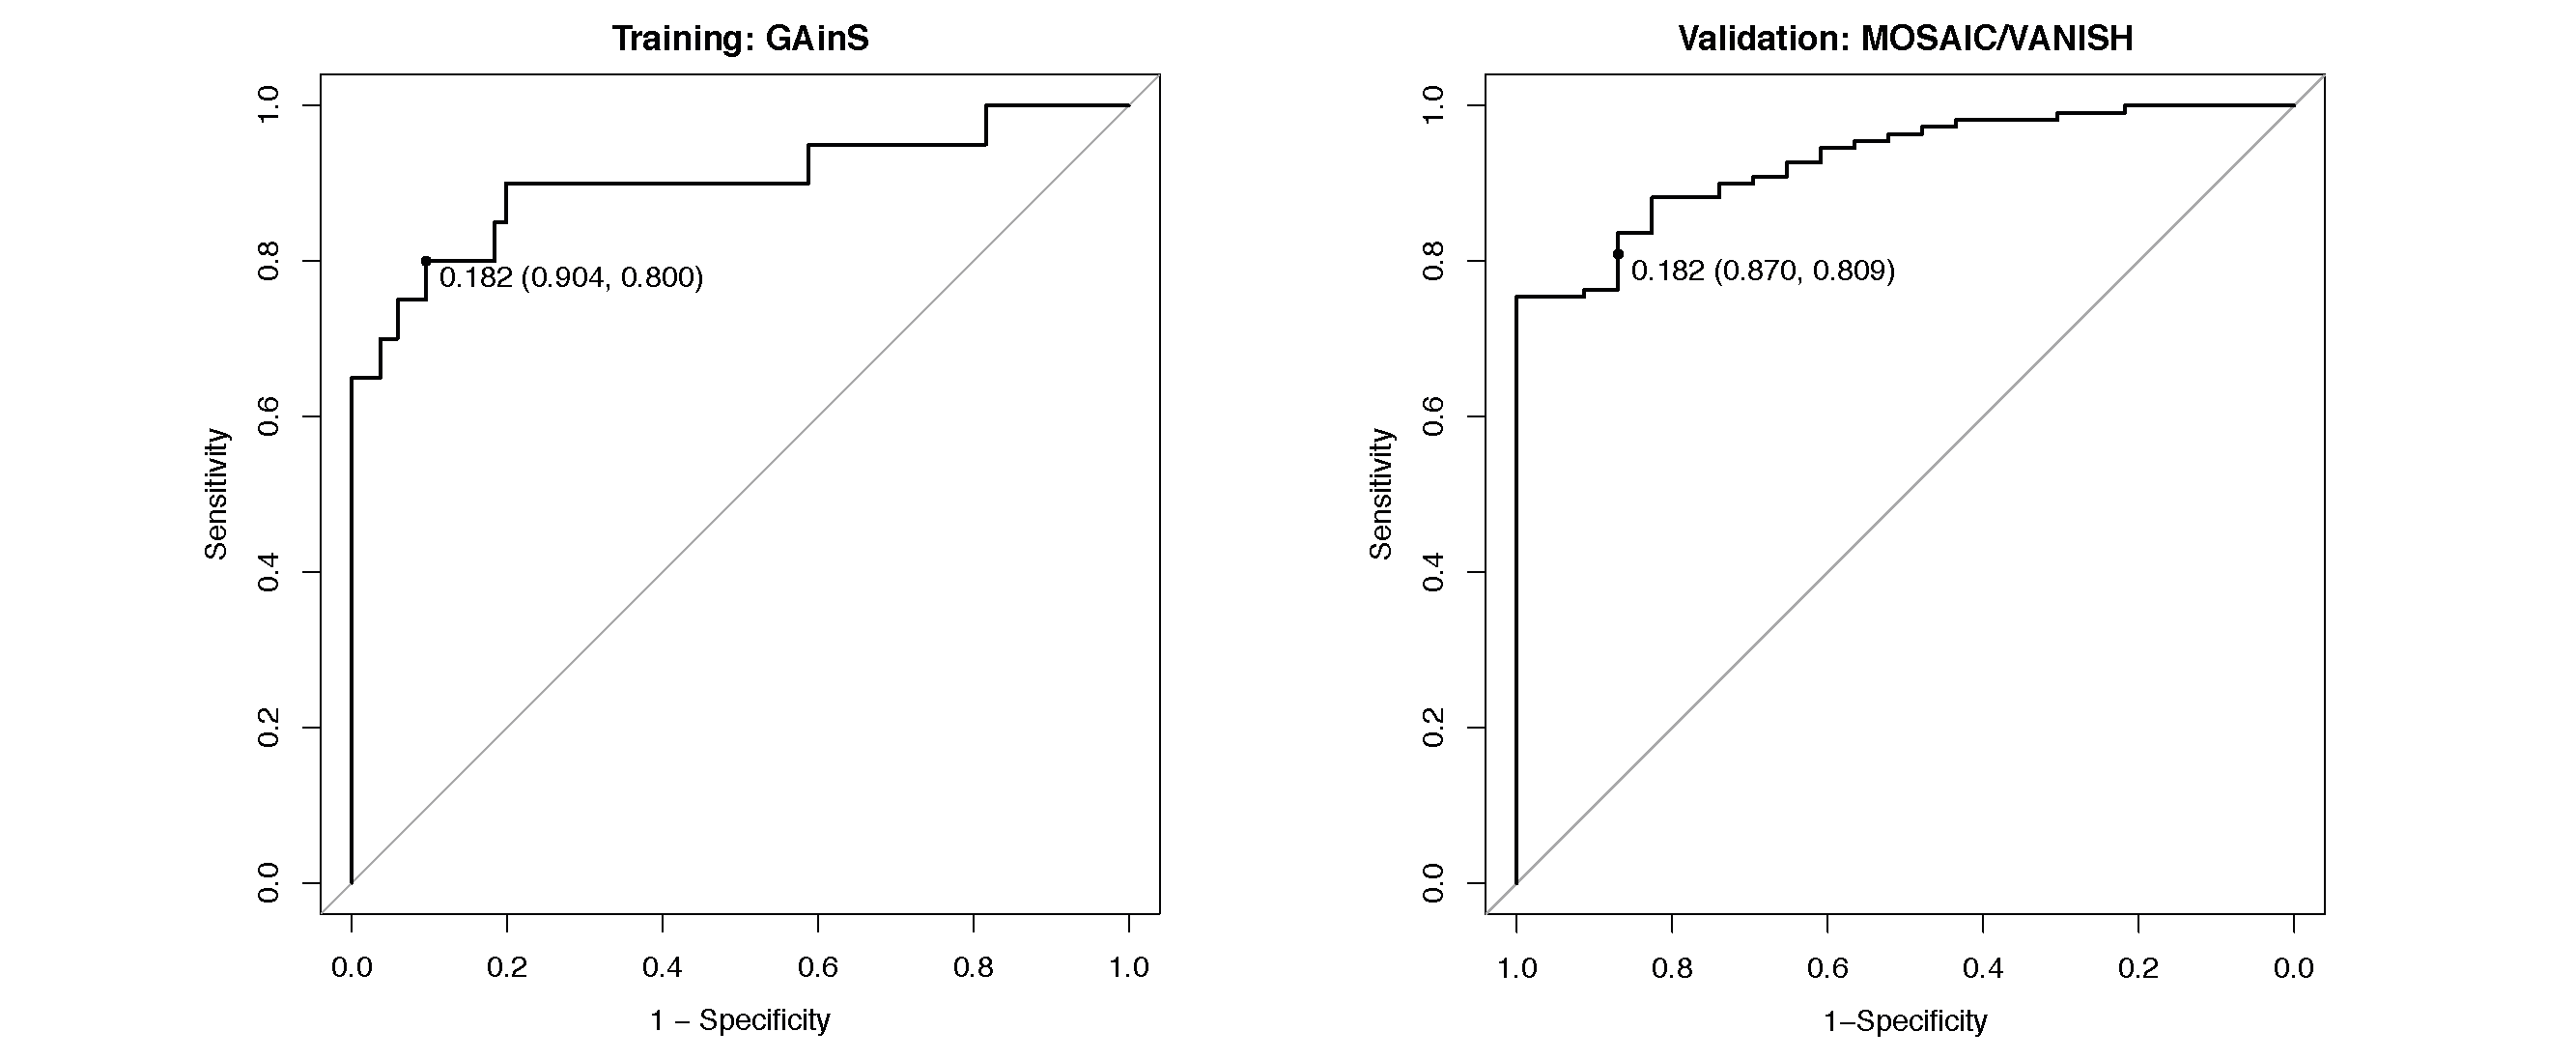
\includegraphics[width=\textwidth]{./Results3/Images/roc-flu-both.png}
\caption[ROC analysis for influenza vs bacterial signature]{\textbf{ROC analysis for influenza vs bacterial signature.} The threshold for discriminating bacterial from influenza infection is noted (0.182), together with the specificity and sensitivity at that threshold in brackets. AUC for the training cohort was 90.1\% (95\% CI 80.4\%-99.8\%) whilst AUC for the combined validation cohort was 92.9\% (95\% CI 88.5\%-97.4\%). MR was 10.9\% for the training cohort and 18\% for the validation cohort.}
\label{fig:roc-flu}
\end{figure}
\FloatBarrier
 
\subsection{Transcriptomic signature of influenza vs viral infection}
Gene expression of individuals with influenza infection (n=20) was contrasted with that of individuals with non-influenza viral infection (n=10). There were no differentially expressed probes at FDR $<$0.05 and fold change $>$1.5 (Figure ~\ref{fig:vp-flu-viral}).

\FloatBarrier
\begin{figure}[htbp]
\centering
\includegraphics[width=\textwidth]{./Results3/Images/vp-flu-viral.pdf}
\caption[Volcano plot of differentially expressed probes in influenza vs viral infection]{\textbf{Volcano plot of differentially expressed probes in influenza vs viral infection.} There are no differentially expressed probes at an FDR $<$0.05 and fold change $>$1.5.}
\label{fig:vp-flu-viral}
\end{figure}
\FloatBarrier

\subsection{Transcriptomic signature of \textit{Streptococcus pneumoniae} infection}
Total leukocyte gene expression was compared between individuals with \textit{S. pneumoniae} infection (n=50) diagnosed by either clinical microbiology or metagenomics and individuals without \textit{S. pneumoniae} infection (n=113). The comparator group included individuals with viral infections and non-pneumococcal bacterial infections. Three patients co-infected with \textit{S. pneumoniae} and another organism were excluded from the analysis.

Differential expression analysis revealed no differentially expressed genes between the two groups (FDR $<$0.05 and fold change $>$1.5).

\FloatBarrier
\begin{figure}[htbp]
\centering
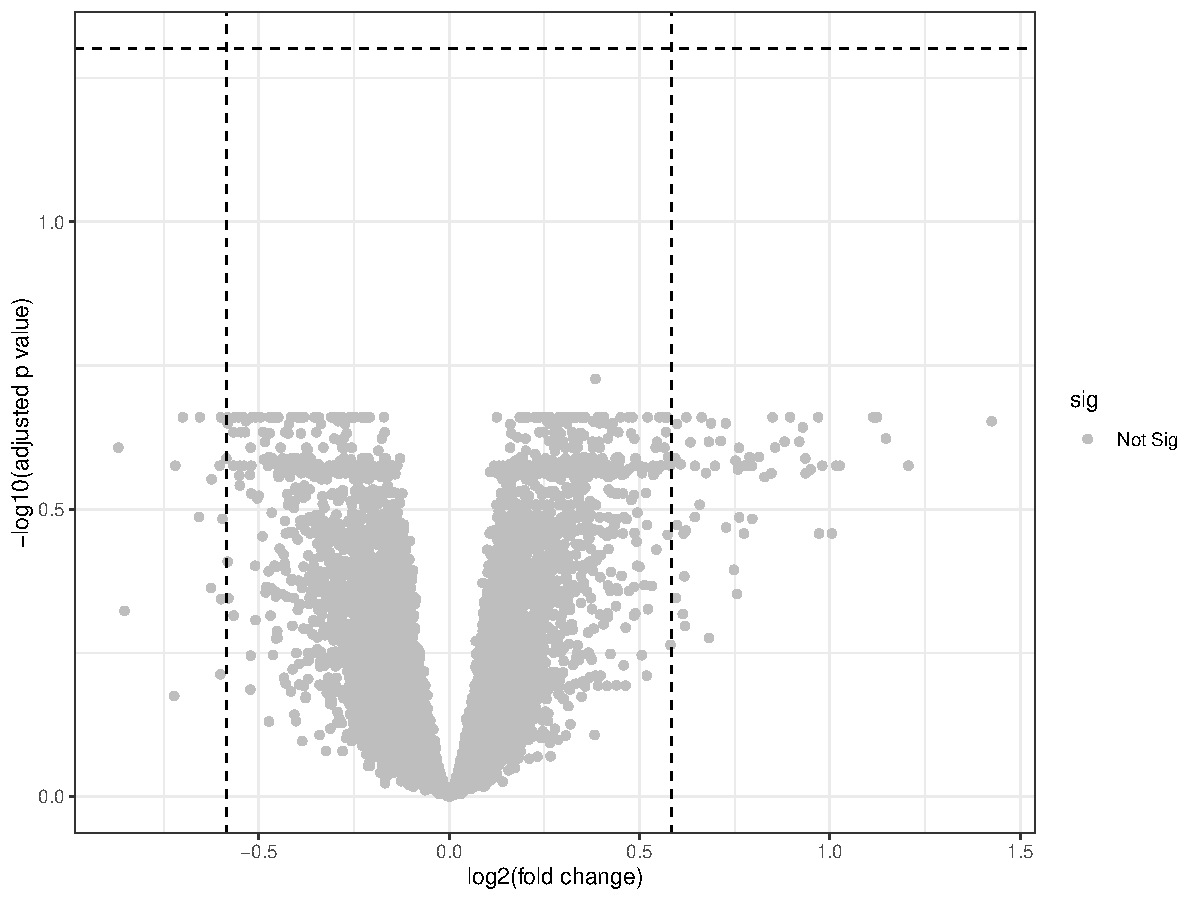
\includegraphics[width=\textwidth]{./Results3/Images/vp-strep.pdf}
\caption[Volcano plot of differentially expressed probes in \textit{S. pneumoniae} infection]{\textbf{Volcano plot of differentially expressed probes in \textit{S. pneumoniae} vs non-\textit{S. pneumoniae} infection.} There are no differentially expressed probes at an FDR $<$0.05 and fold change $>$1.5.}
\label{fig:vp-viral-bacterial}
\end{figure}
\FloatBarrier


\subsection{Genomics: association with HLA}
For this section, the training dataset included 613 individuals with HLA imputed from genotyping data or HLA typing from sequencing data whilst the validation dataset included 274 individuals genotyped separately from the training cohort, with HLA imputation from the genotyping data. Alleles were tested for association with the phenotype of interest if they were present in the training cohort at a prevalence of $\geq$2\%.

\textbf{Influenza.} In the training cohort (n=613), there were 30 individuals with and 583 individuals without a diagnosis of influenza sepsis. Sixty-two HLA class I (HLA-A, HLA-B, HLA-C) and class II (HLA-DQA1, HLA-DQB1, HLA-DRB1) alleles were tested for association at 2-digit resolution. After correction for multiple testing, two alleles (B*35 and C*12) had a statistically significant association with influenza sepsis (Chi-squared test; adjusted p=0.00152 and adjusted p=0.00214 respectively). 

The two alleles were subsquently tested for association with influenza sepsis in the validation cohort (n=274) where there were 33 individuals with and 241 individuals without a diagnosis of influenza sepsis. Here, there was a statistically significant association for B*35 (p=0.0256) but not for C*12 (p=0.352 in the opposite direction) with the presence of influenza sepsis. 

HLA-B*35 is present in the England Leeds cohort (n=5024) at a prevalence of 12.7\% \parencite{AlleleFrequencies}. This was similar to the prevalence of 12.6\% observed in the GAinS training cohort (n=76/611 heterozygous, 1/611 homozygous). There was an increased prevalence of the allele in the influenza positive individuals in the training cohort (n=6/30 heterozygous, 1/30 homozygous; 23.3\%) as well as the validation cohort (n=4/33 heterozygous, 1/33 homozygous; 15.2\%) (Figure ~\ref{fig:bar-hla-b35}).

\FloatBarrier
\begin{figure}[htbp]
\centering
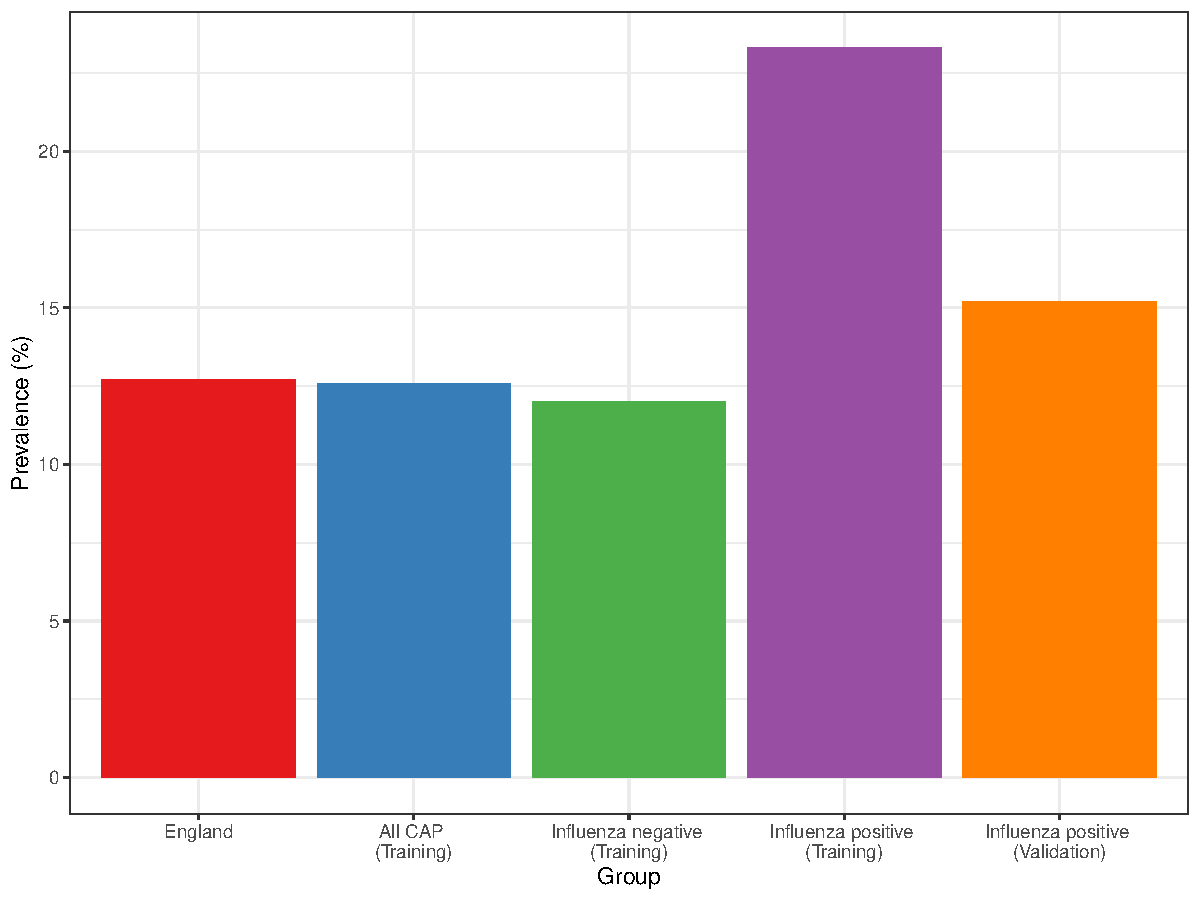
\includegraphics[scale=0.5]{./Results3/Images/bar_hla_b35.pdf}
\caption[Bar graph of HLA-B*35 prevalence]{\textbf{Bar graph of HLA-B*35 prevalence.} The percentage of individuals with at least one HLA-B*35 allele is plotted on the y-axis.}
\label{fig:bar-hla-b35}
\end{figure}
\FloatBarrier

It was not possible to contrast the prevalence of HLA-B*35 between influenza positive and negative individuals at four digit resolution due to small patient numbers.

\textbf{\textit{Streptococcus pneumoniae.}} In the training cohort (n=613), there were 113 individuals with and 500 individuals without a diagnosis of \textit{S. pneumoniae} sepsis. Sixty-two HLA class I (HLA-A, HLA-B, HLA-C) and class II (HLA-DQA1, HLA-DQB1, HLA-DRB1) alleles were tested. After correction for multiple testing, there were no statistically significant associations with \textit{S. pneumoniae} sepsis.

\textbf{EBV reactivation.} Of the 613 individuals in the training cohort, there was EBV reactivation data on 547 individuals (n=197 EBV positive; n=350 EBV negative). Sixty-three HLA class I (HLA-A, HLA-B, HLA-C) and class II (HLA-DQA1, HLA-DQB1, HLA-DRB1) alleles were tested for association. After correction for multiple testing, only one allele (B*07) approached statistical significance (Chi-squared test; adjusted-p=0.0733). 

There were 166 individuals in the validation cohort for whom EBV reactivation data was available (n=68 EBV positive; n=98 EBV negative). HLA-B*07 was tested for association with EBV status and again the result did not reach statistical significance (p=0.102).

\section{Discussion}
\subsection{EBV reactivation and immunosuppression}
Viral reactivation in sepsis has not previously been described in the literature within the context of host gene expression. EBV reactivation in sepsis is common, increases over time and is associated with longer ICU stays and increased mortality. Consistent with the concept that viral reactivation in sepsis is a consequence of immune compromise, EBV reactivation was more frequent in those with the SRS1 immunocompromised sepsis transcriptomic endotype. Differences in the molecular response to EBV reactivation are also seen, in terms of total leukocyte gene expression profiles, with a small number of differentially expressed genes (n=13) between the EBV-positive and EBV-negative individuals. Although a number of these genes are of unknown function, \textit{CACNAD3, CDC20, KIAA0101} and \textit{PRTN3} are all implicated in EBV pathophysiology. In clinical practice, viral reactivation in the critically ill is generally considered to be an epiphenomenon and a marker of illness severity that is of little clinical significance. It remains unclear whether reactivated viruses contribute to the pathophysiology of the host response to sepsis and whether specific treatment is indicated. 

In previously published work, the SRS endotype have been described as categorical traits \parencite{Davenport2016}. Here, it is described for the first time as a continuous phenotype. By using the values of principal component 1, which separates patients with SRS1 from SRS2 in principal component analysis, it was shown that individuals with a more pronounced SRS1 phenotype are more likely to demonstrate reactivation of EBV, most likely as a consequence of decreased immune competence. One area for future work should therefore be to use immunophenotyping to determine whether higher levels of viraemia are associated with increased markers of immunosuppression.

The observed association between EBV reactivation and both morbidity and mortality highlights the clinical importance of this phenomenon. There was an increase in 28-day mortality in individuals with EBV reactivation compared to those without (27\% vs 20\%; p=0.04). This is in keeping with one small study of critically ill sepsis and non-sepsis patients \parencite{Libert2015} although two larger studies focusing on sepsis patients  \parencite{Walton2014} \parencite{Ong2017} did not find an association between EBV reactivation and mortality. EBV-positive patients also had increased levels of organ dysfunction compared with EBV-negative patients. This is in keeping with the findings of Walton and colleagues \parencite{Walton2014} who describe a similar association with SOFA score.

In the overall cohort of 573 patients, an overall 37\% incidence of EBV reactivation was observed. This finding is consistent with other studies in which the incidence of EBV reactivation in plasma has been estimated at 32-48\% \parencite{Walton2014} \parencite{Ong2017}. In contrast, a lower rate of EBV and other viral reactivation was observed in the metagenomic cohort. This is most likely because sample selection for metagenomics prioritised the sequencing of earlier time point samples to enable microbiological diagnosis of CAP with 40\% of samples obtained on the first day of ICU admission. Walton and colleagues \parencite{Walton2014} observed that the median time to reactivation for EBV was 5 days, so it is highly probably that samples EBV-negative on day one would become EBV-positive at later timepoints.

These findings have some potential implications for the management of sepsis. The switch from latency to lytic replication requires the virus to escape from host immune surveillance. In EBV-positive patients, an SRS1 phenotype is associated with higher levels of viraemia, with 17 SRS1 individuals having EBV loads of >10$^3$ copies/ml (vs 11 in the SRS2 group). These levels of viraemia are considerable and prompt the question as to whether such levels are detrimental, perhaps because they compromise host immunity and warrant specific treatment. For example, it is known that EBV reactivation is associated with increased expression of proteins such as an IL-10 homologue which inhibits monocyte/macrophage function \parencite{Moore2001} and several proteins which impair interferon alpha and gamma release \parencite{Morrison2001} \parencite{Cohen1999}. Importantly however, a trial of specific antiviral therapy in CMV reactivation had to be terminated early due to increased mortality in the treatment arm \parencite{Cowley2017}.

Finally, immune therapies for sepsis have been and continue to undergo evaluation and it is likely that an individualised approach will be required. We propose that serial qPCR of EBV viral loads in the clinical setting be considered as part of a biomarker panel to comprehensively assess a patient's immune status, such as that being used in the REAnimation Low Immune Status Markers (REALISM) project \parencite{Rol2017}.

\subsection{\textit{Streptococcus pneumoniae} infection and sepsis endotype}

For patients with \textit{S. pneumoniae} infection where there was detectable bacterial load in plasma by ddPCR, there was a difference in bacterial load depending on SRS endotype, with SRS1 patients displaying higher levels of \textit{S. pneumoniae} bacteraemia. This is in keeping with the SRS1 endotype being associated with a relatively immunosuppressed transcriptomic phenotype, which could potentially reduce the ability of the host immune system to control levels of infection. 

Rello and colleagues \parencite{Rello2009} showed that \textit{S. pneumoniae} bacterial load was independently associated with morbidity and mortality in patients with pneumococcal CAP. Individuals with a \textit{S. pneumoniae} bacterial load of $\geq$10$^3$ copies/ml had an increased risk for septic shock (OR 8.00), the need for mechanical ventilation (OR 10.50), and hospital mortality (OR 5.43).

In the GAinS cohort, there was no association seen between ddPCR \textit{S. pneumoniae} positivity and vasopressor use, mechanical ventilation or 28-day mortality. This remained the case even when individuals with a bacterial load of $\geq$10$^3$ copies/ml were compared to those with a bacterial load below this threshold. 

The disparity between these results and those of Rello and colleagues may be due to two reasons. Firstly, the GAinS patients received antibiotics prior to sample collection so ddPCR-measured bacterial load almost certainly did not reflect peak bacteraemia levels. Secondly, the analysis was limited by only 10 patients in the high bacterial load group, so there might not have been sufficient power to detect a statistically significant difference between the groups. 

However, Rello and colleagues' results are still relevant in that they indicate an association between bacterial load and disease severity. This supports the finding that individuals in the GAinS cohort with the higher mortality SRS1 endotype have higher bacterial loads; these are individuals with greater sepsis severity, reflected in degree of immunosuppression and corresponding \textit{S. pneumoniae} bacterial load.

\subsection{Transcriptomic signatures of infection}
The four contrasts made are summarised in Table ~\ref{tab:dex-summary}.

\FloatBarrier
\begin{table}[]
\begin{center}
\begin{tabular}{|c|c|c|}
\hline
Comparison (no. of patients)                                                             & Patients & \begin{tabular}[c]{@{}c@{}}Differentially \\ expressed probes\end{tabular} \\ \hline
Viral (30) vs bacterial (136)                                                            & 166      & 206                                                                        \\ \hline
Influenza (20) vs bacterial (136)                                                        & 156      & 139                                                                        \\ \hline
Influenza (20) vs viral (10)                                                             & 30       & 0                                                                          \\ \hline
\begin{tabular}[c]{@{}c@{}}S. pneumoniae (50) vs \\ non-S. pneumoniae (113)\end{tabular} & 163      & 0                                                                          \\ \hline
\end{tabular}
\end{center}

\caption[Summary of differential expression analysis]{\textbf{Summary of differential expression analysis.} Differentially expressed probes defined as those with FDR $<$0.05 and fold change $>$1.5.}
\label{tab:dex-summary}
\end{table}


Previous work had identified a six gene signature for differentiating viral from non-viral infection which performed with a reasonable MR (9.1\%). However, there were serious limitations to this analysis in that the "non-viral" comparator group was poorly defined, with approximately half lacking a microbiological diagnosis.

This work was improved upon by better microbiological phenotyping (primarily through metagenomics and curation of clinical data) and an increase in cohort size with the addition of three further gene expression datasets. This resulted in the viral vs bacterial comparison yielding 206 differentially expressed genes at FDR $<$0.05 and fold change $>$1.5 (previous work had identified only 2 differentially expressed probes at FDR $<$0.05 and fold change $>$1.2). 

Two predictive gene expression signatures were identified using the elastic net method. The viral vs bacterial signature performed reasonably well in the validation cohort (MR 9.8\%) whilst the influenza vs bacterial signature performed less well, with a higher MR of 18\% in the validation cohort. 

Of the 10 genes identified in the viral vs bacterial signature, a number are of particular relevance to viral infection, increasing our confidence in the predictive gene set. \textit{IFI27}, encodes an interferon alpha-inducible protein which has been described as a biomarker for differentiating influenza from bacterial respiratory infection \parencite{Tang2017}. \textit{SRC} encodes a non-receptor tyrosine kinase protein that interacts with viral proteins mediating key host-pathogen interactions \parencite{Pagano2013}.

There were no differentially expressed genes identified in the influenza vs viral analysis or the \textit{S. pneumoniae} vs non-\textit{S. pneumoniae} analysis. This parallels the results from previous work (Subsection \ref{sssec:emmaDEgenes}) which identified only 2 differentially expressed genes in influenza vs viral infection and none in Gram-positive vs Gram-negative infections. It is possible that our modest patient numbers meant there was insufficient power to detect a difference between the different classes of infection. Alternatively, these results suggest that the transcriptomic response in sepsis may be attributable to the class of infection (i.e. viral or bacterial) rather than specific to individual organisms. This is supported by published work describing a lack of genes differentiating Gram-positive from Gram-negative sepsis \parencite{Tang2008}. 

\subsection{Genomics: association with HLA}
An association between HLA-B*35 positivity and influenza sepsis was detected in both training and validation cohorts. This finding has not previously been described in sepsis patients or in a Caucasian population. However, a case-control study (n=138 cases vs n=225 controls) of the influenza A H1N1/09 pandemic found that B*35:01:01-C*07:02:01 was one of two haplotypes observed at higher frequency in H1N1/09 influenza patients from a Mexican population \parencite{Falfan-Valencia2018}. Similarly, a case-control study of influenza A H1N1/09 pandemic patients in north-east India observed the frequency of HLA-B*35 to be higher in cases (n=35) versus controls (n=35). This preliminary finding in the GAinS cohort should be treated with caution and future work would include validating the finding in a cohort with larger numbers of influenza cases, restricting the analysis to Caucasian individuals and consideration of haplotype structure.

A possible association between HLA-B*07 positivity and EBV reactivation was detected in the GAinS cohort. Although this did not reach statistical significance, evidence in the literature is suggestive of this being a genuine finding. In multiple sclerosis, where EBV plays a critical role in disease development, HLA-B*07 is found at higher prevalence in a patients compared with controls \parencite{Jilek2012}. In the same Swiss cohort, ex vivo studies showed that the HLA-B*07 restricted EBV-specific CD8+ T cell response was dysregulated in multiple sclerosis patients \parencite{Jilek2012}. In another study \parencite{Agostini2018}, EBV viral load was higher in multiple sclerosis patients positive for HLA-B*07 compared to those negative for the allele.

No association between HLA class I and II alleles and \textit{S. pneumoniae} infection was detected. This is consistent with the literature, where no positive associations have been described. A possible reason for the positive findings in viral infection but negative finding in bacterial infection may be that an effective host response against viruses relies more heavily on cell-mediated immunity through class I and class II HLA molecules. 
 
\section{Conclusions}
Improved microbiological phenotyping has the potential to enhance our understanding of the host response in sepsis. In this chapter, I have explored the interaction between microbiology and host transcriptomic sepsis endotypes, performed differential gene expression analysis for different classes of infection, and investigated the effect of HLA alleles on susceptibility to different microbiological classes of infection. The results have shown integrating metagenomic data with other -omic datasets to be a promising approach. 

\chapter{General Discussion}
\label{ch:Discussion}
\textit{This chapter outlines the broader conclusions and future directions suggested by the work described in this thesis}

\startcontents[chapters]{\vspace{-1.4cm}}
\singlespacing
\printcontents[chapters]{}{1}{\section*{ }\setcounter{tocdepth}{1}}
\doublespacing
\vspace{0.5cm}

General intro

\section{A section}

\section{Limitations and future work}

\section{Conclusion}

Conclusions.
\appendix
\addcontentsline{toc}{chapter}{Appendices}

\singlespacing

\chapter{Materials and Methods}\label{app:Methods}
\begin{center}
\begin{landscape}

\begin{table}[htbp]
\begin{tabular}{|l|l|l|l|}
\hline
Organism               & Amplicon & Primer/probe                                                                           & Nucleotide sequence                                                                                                                                                               \\ \hline
\textit{S. pneumoniae} & 67 bp         & \begin{tabular}[c]{@{}l@{}}Taqman probe\\ Forward primer\\ Reverse primer\end{tabular} & \begin{tabular}[c]{@{}l@{}}5'-/5HEX/AAT GTT ACG/ZEN/CAA CTG ACG AG/3IABkFQ/-3'\\ 5'-GCT GTT TTA GCA GAT AGT GAG ATC GA-3'\\ 5'-TCC CAG TCG GTG CTG TCA-3'\end{tabular}            \\ \hline
Influenza A            & 185 bp        & \begin{tabular}[c]{@{}l@{}}Taqman probe\\ Forward primer\\ Reverse primer\end{tabular} & \begin{tabular}[c]{@{}l@{}}5'-/56-FAM/TGC AGT CCT/ZEN/CGC TCA CTG GGC ACG /3IABkFQ/-3'\\ 5'-AGG GCA TTY TGG ACA AAK CGT CTA-3'\\ 5'-GAC CRA TCC TGT CAC CTC TGA C-3'\end{tabular} \\ \hline
Epstein-Barr virus     & 75 bp         & \begin{tabular}[c]{@{}l@{}}Taqman probe\\ Forward primer\\ Reverse primer\end{tabular} & \begin{tabular}[c]{@{}l@{}}5'-/56-FAM/AGG GAG ACA/ZEN/CAT CTG GAC CAG AAG GC/3IABkFQ/-3'\\ 5'-TCT TTG AGG TCC ACT GCC G-3'\\ 5'-TAC AGG ACC TGG AAA TGG CC-3'\end{tabular}       \\ \hline
Cytomegalovirus        & 66 bp         & \begin{tabular}[c]{@{}l@{}}Taqman probe\\ Forward primer\\ Reverse primer\end{tabular} & \begin{tabular}[c]{@{}l@{}}5'-/56-FAM/TG GGC AAC C/ZEN/A CCG CAC TGA GG/3IABkFQ/-3'\\ 5'-TGG GCG AGG ACA ACG AA-3'\\ 5'-TGA GGC TGG GAA GCT GAC AT-3'\end{tabular}                \\ \hline
\end{tabular}
\medskip
\caption[Primer/probe sets used for the digital droplet PCR experiments]{\textbf{Primer/probe sets used for the digital droplet PCR experiments}}
\label{tab:ddPCRprobes}
\end{table}
\end{landscape}
\bigskip
\newpage





\chapter{Application of Metagenomic Sequencing to Sepsis Samples}
\label{app:Results1}


\begin{table}[]
\scalebox{0.7}{
\begin{tabular}{|l|l|}
\hline
\textbf{Virus family} & \textbf{Virus species}                                                                                                                                                                                                                                                                                   \\ \hline
Adenoviridae          & Human adenovirus                                                                                                                                                                                                                                                                                         \\ \hline
Arenaviridae          & \begin{tabular}[c]{@{}l@{}}Lassa virus\\ Lymphocytic choriomeningitis virus\end{tabular}                                                                                                                                                                                                                 \\ \hline
Coronaviridae         & \begin{tabular}[c]{@{}l@{}}Human coronavirus HKU1, NL63, OC43, 229E\\ Middle East respiratory syndrome coronavirus\\ Severe acute respiratory syndrome coronavirus\end{tabular}                                                                                                                          \\ \hline
Flaviviridae          & \begin{tabular}[c]{@{}l@{}}Dengue virus\\ Japanese encephalitis virus\\ Murray Valley encephalitis virus\\ St Louis encephalitis virus\\ Tick-borne encephalitis virus\\ West Nile virus\\ Yellow fever virus\\ Zika virus\end{tabular}                                                                  \\ \hline
Herpesviridae         & \begin{tabular}[c]{@{}l@{}}Human herpesvirus 3 (Varicella zoster virus)\\ Human herpesvirus 4 (Epstein Barrvirus)\\ Human herpesvirus 5 (Cytomegalovirus)\\ Human herpesvirus 6-7 (Roseolovirus)\\ Human herpesvirus 8 (Kaposi's sarcoma-associated herpesvirus)\\ Herpes simplex virus 1-2\end{tabular} \\ \hline
Orthomyxoviridae      & Influenza virus A-C                                                                                                                                                                                                                                                                                      \\ \hline
Paramyxoviridae       & \begin{tabular}[c]{@{}l@{}}Hendra henipavirus\\ Human metapneumovirus \\ Humanparainfluenzavirus1-5\\ Measles morbilivirus\\ Mumps rubulavirus\\ Nipah henipavirus\\ Respiratory syncytial virus \\ Sosugavirus\end{tabular}                                                                             \\ \hline
Parvoviridae          & \begin{tabular}[c]{@{}l@{}}Human bocavirus\\ Human parvovirus B19\\ Human parvovirus 4\\ Primate erythroparvovirus 1\\ Primate tetraparvovirus 1\end{tabular}                                                                                                                                            \\ \hline
Peribunyaviridae      & California encephalitis virus                                                                                                                                                                                                                                                                            \\ \hline
Phenuiviridae         & \begin{tabular}[c]{@{}l@{}}Rift valley fever virus\\ Sandfly fever Naples virus\\ Sandfly fever Sicilian virus\end{tabular}                                                                                                                                                                              \\ \hline
Picornaviridae        & \begin{tabular}[c]{@{}l@{}}Cardiovirus A-B\\ Coxsackie A virus\\ ECHO virus\\ Enterovirus A, B, D\\ Hepatitis A virus\\ Parechovirus A-B \\ Rhinovirus A-C\\ Rosavirus A\\ Salivivirus\end{tabular}                                                                                                      \\ \hline
Polyomaviridae        & \begin{tabular}[c]{@{}l@{}}BK virus\\ JC polyomavirus\end{tabular}                                                                                                                                                                                                                                       \\ \hline
Reoviridae            & Rotavirus A-C                                                                                                                                                                                                                                                                                            \\ \hline
Rhabdovirus           & \begin{tabular}[c]{@{}l@{}}Australian bat lyssavirus\\ Duvenhage lyssavirus\\ European bat lyssavirus 1-2\\ Lagos bat lyssavirus\\ Mokola lyssavirus\\ Rabies lyssavirus\end{tabular}                                                                                                                    \\ \hline
Togaviridae           & \begin{tabular}[c]{@{}l@{}}Chikungunya virus\\ Eastern equine encephalitis virus\\ Rubella virus\\ Venezuelan equine encephalitis virus\\ Western equine encephalitis virus\end{tabular}                                                                                                                 \\ \hline
\end{tabular}
}
\caption[Enrichment Probe Set Viruses]{\textbf{Viruses included in enrichment probe set}}
\label{tab:ProbeSetViruses}
\end{table}

\begin{table}[]
\begin{tabular}{|l|l|}
\hline
\textbf{Bacterial genus}  & \textbf{Bacterial species}                                                             \\ \hline
\textit{Acinetobacter}    & \textit{\begin{tabular}[c]{@{}l@{}}baumanii\\ calcoaceticus\end{tabular}}              \\ \hline
\textit{Bartonella}       & \textit{henselae}                                                                      \\ \hline
\textit{Bordetella}       & \textit{pertussis}                                                                     \\ \hline
\textit{Borrelia}         & \textit{burgdorferi}                                                                   \\ \hline
\textit{Brucella}         & \textit{}                                                                              \\ \hline
\textit{Burkholderia}     & \textit{cepacia}                                                                       \\ \hline
\textit{Chlamydophila}    & \textit{\begin{tabular}[c]{@{}l@{}}pneumoniae\\ psittaci\end{tabular}}                 \\ \hline
\textit{Coxiella}         & \textit{burnetii}                                                                      \\ \hline
\textit{Enterobacter}     & \textit{\begin{tabular}[c]{@{}l@{}}aerogenes\\ cloacae\end{tabular}}                   \\ \hline
\textit{Escherichia}      & \textit{coli}                                                                          \\ \hline
\textit{Haemophilus}      & \textit{\begin{tabular}[c]{@{}l@{}}influenzae\\ parainfluenzae\end{tabular}}           \\ \hline
\textit{Klebsiella}       & \textit{\begin{tabular}[c]{@{}l@{}}pneumoniae\\ oxytoca\end{tabular}}                  \\ \hline
\textit{Legionella}       & \textit{pneumophila}                                                                   \\ \hline
\textit{Leptospira}       & \textit{}                                                                              \\ \hline
\textit{Listeria}         & \textit{monocytogenes}                                                                 \\ \hline
\textit{Moraxella}        & \textit{catarrhalis}                                                                   \\ \hline
\textit{Mycobacterium}    & \textit{\begin{tabular}[c]{@{}l@{}}avium\\ intracellulare\\ tuberculosis\end{tabular}} \\ \hline
\textit{Mycoplasma}       & \textit{pneumoniae}                                                                    \\ \hline
\textit{Neisseria}        & \textit{meningitidis}                                                                  \\ \hline
\textit{Nocardia}         & \textit{}                                                                              \\ \hline
\textit{Pseudomonas}      & \textit{aeruginosa}                                                                    \\ \hline
\textit{Serratia}         & \textit{marcescens}                                                                    \\ \hline
\textit{Staphylococcus}   & \textit{aureus}                                                                        \\ \hline
\textit{Stenotrophomonas} & \textit{maltophilia}                                                                   \\ \hline
\textit{Streptococcus}    & \textit{\begin{tabular}[c]{@{}l@{}}agalactiae\\ pneumoniae\\ pyogenes\end{tabular}}    \\ \hline
\textit{Treponema}        & \textit{pallidum}                                                                      \\ \hline
\end{tabular}
\caption[Enrichment Probe Set Bacteria]{\textbf{Bacteria included in enrichment probe set}}
\label{tab:ProbeSetBacteria}
\end{table}




\begin{landscape}


\begin{table}[]
\centering
\caption[Viral Multiplex Reference]{Viral Multiplex Reference reagent 11/242 (UK NIBSC). This reference set included 25 viruses of various nucleic acid types, envelope types and genome sizes. 21/25 viruses had corresponding enrichment probes in our probe panel. (Adapted from Mee et al.)
\label{tab:VMR}\\
{\bf }}
\scalebox{0.85}{
\begin{tabular}{|l|l|l|l|l|l|l|}
\hline
Group                      & Family                            & Species/serotype               & Envelope             & Genome size & Included in probeset & Concentration (log10 copies/ml) \\ \hline
\multirow{7}{*}{dsDNA}     & \multirow{2}{*}{Adenoviridae}     & Adenovirus 2                   & \multirow{2}{*}{No}  & 35.9        & Yes                  & NA                                           \\ \cline{3-3} \cline{5-7} 
                           &                                   & Adenovirus 41                  &                      & 34.2        & Yes                  & NA                                           \\ \cline{2-7} 
                           & \multirow{5}{*}{Herpesviridae}    & Human herpesvirus 1            & \multirow{5}{*}{Yes} & 151.2       & Yes                  & NA                                           \\ \cline{3-3} \cline{5-7} 
                           &                                   & Human herpesvirus 2            &                      & 154.7       & Yes                  & NA                                           \\ \cline{3-3} \cline{5-7} 
                           &                                   & Human herpesvirus 3 (VZV)      &                      & 124.8       & Yes                  & NA                                           \\ \cline{3-3} \cline{5-7} 
                           &                                   & Human herpesvirus 4 (EBV)      &                      & 171.7       & Yes                  & 3.88                                         \\ \cline{3-3} \cline{5-7} 
                           &                                   & Human herpesvirus 5 (CMV)      &                      & 233.7       & Yes                  & 4.66                                         \\ \hline
dsRNA                      & Reoviridae                        & Rotavirus A                    & No                   & 18.5        & Yes                  & 6.76                                         \\ \hline
\multirow{8}{*}{ssRNA (+)} & Astroviridae                      & Astrovirus                     & No                   & 6.8         & No                   & NA                                           \\ \cline{2-7} 
                           & \multirow{3}{*}{Caliciviridae}    & Norovirus GI                   & \multirow{3}{*}{No}  & 7.6         & No                   & NA                                           \\ \cline{3-3} \cline{5-7} 
                           &                                   & Norovirus GII                  &                      & 7.5         & No                   & NA                                           \\ \cline{3-3} \cline{5-7} 
                           &                                   & Sapovirus C12                  &                      & 7.5         & No                   & NA                                           \\ \cline{2-7} 
                           & Coronaviridae                     & Coronavirus 229E               & Yes                  & 27.2        & Yes                  & NA                                           \\ \cline{2-7} 
                           & \multirow{3}{*}{Picornaviridae}   & Coxsackievirus B4              & \multirow{3}{*}{No}  & 7.4         & Yes                  & NA                                           \\ \cline{3-3} \cline{5-7} 
                           &                                   & Rhinovirus A39                 &                      & 7.1         & Yes                  & NA                                           \\ \cline{3-3} \cline{5-7} 
                           &                                   & Parechovirus 3                 &                      & 7.2         & Yes                  & 7.07                                         \\ \hline
\multirow{9}{*}{ssRNA (-)} & \multirow{3}{*}{Orthomyxoviridae} & Influenza A virus H1N1         & \multirow{3}{*}{Yes} & 13.2        & Yes                  & NA                                           \\ \cline{3-3} \cline{5-7} 
                           &                                   & Influenza A virus H3N2         &                      & 13.6        & Yes                  & NA                                           \\ \cline{3-3} \cline{5-7} 
                           &                                   & Influenza B virus              &                      & 14.2        & Yes                  & NA                                           \\ \cline{2-7} 
                           & \multirow{6}{*}{Paramyxoviridae}  & Metapneumovirus A              & \multirow{6}{*}{Yes} & 13.3        & Yes                  & NA                                           \\ \cline{3-3} \cline{5-7} 
                           &                                   & Parainfluenzavirus 1           &                      & 15.5        & Yes                  & NA                                           \\ \cline{3-3} \cline{5-7} 
                           &                                   & Parainfluenzavirus 2           &                      & 15.7        & Yes                  & NA                                           \\ \cline{3-3} \cline{5-7} 
                           &                                   & Parainfluenzavirus 3           &                      & 15.4        & Yes                  & NA                                           \\ \cline{3-3} \cline{5-7} 
                           &                                   & Parainfluenzavirus 4           &                      & 17.4        & Yes                  & NA                                           \\ \cline{3-3} \cline{5-7} 
                           &                                   & Respiratory syncytial virus A2 &                      & 15.2        & Yes                  & 3.75                                         \\ \hline
\small
\end{tabular}
}
\end{table}


\end{landscape}

\clearpage

\end{center}

\chapter{Improved Classification of Microbiological Aetiology in Sepsis}
\label{ch:AppResults2}
\begin{figure}[htbp]
\centering
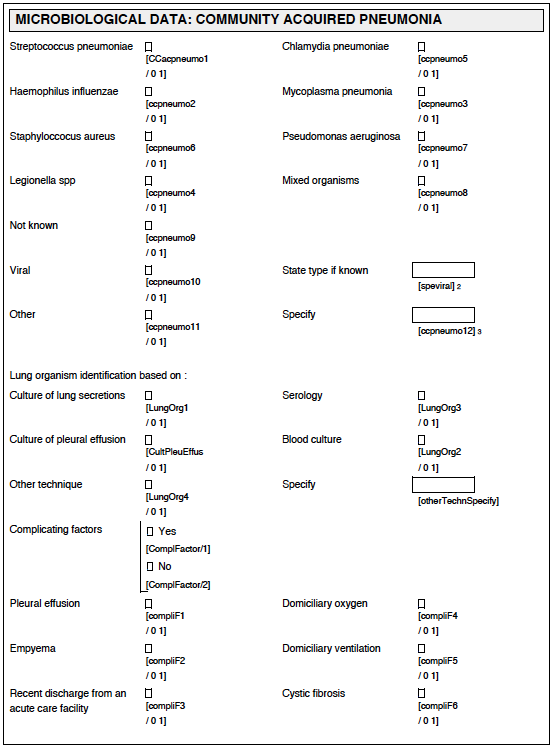
\includegraphics[scale=0.7]{./Appendices/Images/eCRF1.png}
\end{figure}

\begin{figure}[htbp]
\centering
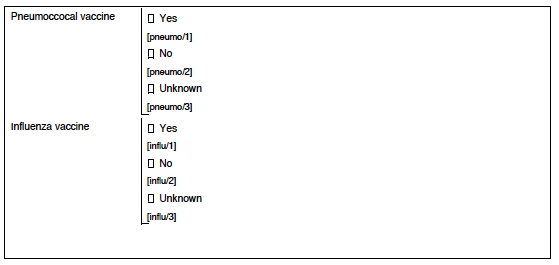
\includegraphics[scale=0.7]{./Appendices/Images/eCRF2.png}
\caption[Electronic case record form]{\textbf{GAinS electronic case record form: microbiology section}}
\label{fig:eCRF}
\end{figure}

\chapter{Integration of Microbiology with the Host Response}\label{ch:AppResults3}

\begin{table}[]
\begin{center}
\begin{tabular}{lll}
\textbf{Gene}      & \textbf{log2(fold change)} & \textbf{FDR} \\
\textit{IGLL1}     & 0.79                       & 4.02E-03     \\
\textit{CDC20}     & 0.62                       & 4.51E-03     \\
\textit{CACNA2D3}  & -0.63                      & 5.21E-03     \\
\textit{TXNDC5}    & 0.75                       & 8.48E-03     \\
\textit{IGKV3D-20} & 0.78                       & 9.23E-03     \\
\textit{KIAA0101}  & 0.59                       & 1.28E-02     \\
\textit{IGKV1D-33} & 0.61                       & 1.33E-02     \\
\textit{IGJ}       & 0.83                       & 1.33E-02     \\
\textit{PRTN3}     & 0.66                       & 4.68E-02    
\end{tabular}
\end{center}
\caption[Differentially expressed genes in EBV reactivation]{\textbf{Summary of differentially expressed genes in EBV-positive vs EBV-negative individuals.} Nine genes were significant at fold-change $>$1.5 and FDR $<$0.05.} 
\label{tab:ebv-de-genes}
\end{table}

\begin{table}[]
\begin{center}
\begin{tabular}{lll}
\textbf{Gene}      & \textbf{log2(fold change)} & \textbf{FDR} \\
\textit{IGLL1}     & 0.85                       & 1.15E-03     \\
\textit{TXNDC5}    & 0.81                       & 2.43E-03     \\
\textit{IGKV3D-20} & 0.84                       & 2.54E-03     \\
\textit{IGKV1D-33} & 0.66                       & 3.38E-03     \\
\textit{CDC20}     & 0.59                       & 3.98E-03     \\
\textit{IGJ}       & 0.89                       & 4.06E-03     \\
\textit{MGC29506}  & 0.61                       & 5.96E-03     \\
\textit{TNFRSF17}  & 0.63                       & 1.32E-02     \\
\textit{DEFA1B} & 0.82                       & 3.11E-02     \\
\textit{PRTN3}     & 0.66                       & 3.87E-02     \\
\textit{DEFA4}     & 0.75                       & 4.19E-02     \\
\textit{CEACAM6}   & 0.63                       & 4.82E-02    
\end{tabular}
\end{center}
\caption[Differentially expressed genes in EBV reactivation with SRS as a covariate]{\textbf{Summary of differentially expressed genes in EBV-positive vs EBV-negative individuals with SRS included as a covariate in the linear model.} Twelve genes were significant at fold-change $>$1.5 and FDR $<$0.05.} 
\label{tab:ebv-de-genes-srs}
\end{table}



\begin{table}
\begin{center}
\scalebox{0.9}{
\begin{tabular}{lll}
\textbf{Gene}      & \textbf{log2(fold change)} & \textbf{FDR} \\
\textit{IFI27}     & 3.10           & 6.88E-07           \\
\textit{IMPA2}     & -0.64          & 1.86E-04           \\
\textit{C3ORF54}   & 0.74           & 6.59E-04           \\
\textit{SPATS2L}   & 1.02           & 6.59E-04           \\
\textit{LOC554203} & 0.59           & 6.91E-04           \\
\textit{HERC6}     & 0.94           & 8.17E-04           \\
\textit{JUP}       & 1.28           & 9.63E-04           \\
\textit{TIMM10}    & 1.33           & 1.03E-03           \\
\textit{SRC}       & 0.77           & 1.03E-03           \\
\textit{HES4}      & 1.04           & 1.03E-03           \\
\textit{LGALS3BP}  & 0.82           & 1.03E-03           \\
\textit{RASGRP3}   & 0.75           & 1.03E-03           \\
\textit{TGIF2}     & 0.64           & 1.03E-03           \\
\textit{MT1A}      & 0.89           & 1.03E-03           \\
\textit{C9ORF91}   & 0.75           & 1.03E-03           \\
\textit{OAS1}      & 1.42           & 1.08E-03           \\
\textit{SCO2}      & 0.92           & 1.08E-03           \\
\textit{HS.125087} & 1.21           & 1.08E-03           \\
\textit{PARP12}    & 1.07           & 1.08E-03           \\
\textit{EPSTI1}    & 2.02           & 1.08E-03           \\
\textit{OAS2}      & 1.57           & 1.08E-03           \\
\textit{IFI44L}    & 2.42           & 1.08E-03           \\
\textit{SP140}     & 0.78           & 1.08E-03           \\
\textit{LY6E}      & 1.69           & 1.11E-03           \\
\textit{CXCL10}    & 0.78           & 1.16E-03           \\
\textit{TMCO3}     & -0.70          & 1.21E-03           \\
\textit{HS.72010}  & 0.63           & 1.28E-03           \\
\textit{XAF1}      & 1.44           & 1.28E-03           \\
\textit{IFI44}     & 1.68           & 1.33E-03           \\
\textit{RNASE1}    & 0.94           & 1.36E-03           \\
\textit{GALM}      & 0.85           & 1.45E-03           \\
\textit{IFIT3}     & 1.57           & 1.45E-03           \\
\textit{RSAD2}     & 1.81           & 1.84E-03           \\
\textit{LAMP3}     & 0.72           & 1.99E-03           \\
\textit{HS.386275} & 0.70           & 1.99E-03           \\
\textit{PLB1}      & -0.74          & 2.02E-03           \\
\textit{MT2A}      & 1.00           & 2.14E-03           \\
\textit{SERPING1}  & 1.50           & 2.14E-03           \\
\textit{OAS3}      & 1.66           & 2.14E-03           \\
\textit{CDKN1A}    & 0.71           & 2.14E-03           \\
\textit{LHFPL2}    & 0.68           & 2.30E-03           \\
\textit{BTN3A3}    & 0.85           & 2.47E-03           \\
\textit{PARP14}    & 0.95           & 2.52E-03           \\
\textit{IFIT5}     & 0.97           & 2.57E-03           \\
\textit{FHL2}      & 0.61           & 2.60E-03           \\
\textit{CXCL16}    & -0.63          & 2.93E-03           \\
\textit{SIGLEC10}  & -0.88          & 3.13E-03           \\
\textit{NLRC4}     & -0.67          & 3.55E-03           \\
\textit{ISG15}     & 1.68           & 3.59E-03           \\
\textit{ZNF684}    & 0.60           & 3.63E-03                  


\end{tabular}}
\end{center}
\caption[Differentially expressed genes in viral infection]{\textbf{Summary of differentially expressed genes in viral vs bacterial infection.} The top 50 most significantly differentially expressed genes are listed here.} 
\label{tab:vb-de-genes}
\end{table}

\begin{table}[]
\begin{center}
\scalebox{0.9}{
\begin{tabular}{lll}
\textbf{Gene}      & \textbf{log2(fold change)} & \textbf{FDR} \\
\textit{IFI27}     & 3.52                       & 1.3E-06      \\
\textit{JUP}       & 1.68                       & 2.0E-04      \\
\textit{C3ORF54}   & 0.90                       & 4.7E-04      \\
\textit{NPL}       & -0.66                      & 7.9E-04      \\
\textit{SPATS2L}   & 1.17                       & 1.1E-03      \\
\textit{CBL}       & -0.68                      & 1.4E-03      \\
\textit{IMPA2}     & -0.67                      & 1.7E-03      \\
\textit{HERC6}     & 1.01                       & 4.8E-03      \\
\textit{LGALS3BP}  & 0.89                       & 5.1E-03      \\
\textit{HES4}      & 1.12                       & 6.0E-03      \\
\textit{MT1A}      & 0.98                       & 6.2E-03      \\
\textit{BCAT1}     & -1.20                      & 7.0E-03      \\
\textit{RASGRP3}   & 0.80                       & 7.0E-03      \\
\textit{ECHDC3}    & -1.25                      & 7.2E-03      \\
\textit{CDC123}    & -0.62                      & 7.2E-03      \\
\textit{MTE}       & 0.64                       & 7.2E-03      \\
\textit{SCO2}      & 1.00                       & 7.2E-03      \\
\textit{SP140}     & 0.83                       & 7.2E-03      \\
\textit{LOC389386} & 0.66                       & 7.2E-03      \\
\textit{GALM}      & 0.95                       & 7.2E-03      \\
\textit{UBQLNL}    & 0.60                       & 7.2E-03      \\
\textit{SOCS2}     & 0.82                       & 7.2E-03      \\
\textit{LY6E}      & 1.83                       & 7.2E-03      \\
\textit{HS.125087} & 1.25                       & 7.2E-03      \\
\textit{OAS2}      & 1.69                       & 7.2E-03      \\
\textit{NUDT5}     & -0.65                      & 7.5E-03      \\
\textit{MT2A}      & 1.12                       & 8.0E-03      \\
\textit{IFI44L}    & 2.55                       & 8.0E-03      \\
\textit{OAS1}      & 1.48                       & 8.0E-03      \\
\textit{ADARB1}    & 0.70                       & 8.0E-03      \\
\textit{LAMP3}     & 0.79                       & 8.0E-03      \\
\textit{LOC401845} & 0.62                       & 8.0E-03      \\
\textit{PARP12}    & 1.11                       & 8.0E-03      \\
\textit{CDKN1A}    & 0.80                       & 8.0E-03      \\
\textit{SLC31A2}   & -0.73                      & 8.0E-03      \\
\textit{CXCL10}    & 0.78                       & 8.0E-03      \\
\textit{FHL2}      & 0.70                       & 8.0E-03      \\
\textit{XAF1}      & 1.51                       & 8.0E-03      \\
\textit{HIST1H4E}  & 0.59                       & 8.0E-03      \\
\textit{DUSP5}     & 0.66                       & 8.1E-03      \\
\textit{TGIF2}     & 0.65                       & 8.6E-03      \\
\textit{PDE9A}     & 0.73                       & 8.9E-03      \\
\textit{HS.72010}  & 0.66                       & 8.9E-03      \\
\textit{IFI44}     & 1.77                       & 9.4E-03      \\
\textit{TIMM10}    & 1.28                       & 9.4E-03      \\
\textit{LOC652694} & 1.34                       & 9.8E-03      \\
\textit{RAB11FIP3} & 0.60                       & 9.8E-03      \\
\textit{CD69}      & 0.86                       & 1.0E-02      \\
\textit{SRC}       & 0.74                       & 1.0E-02      \\
\textit{OAS3}      & 1.79                       & 1.0E-02     
\end{tabular}}
\end{center}
\caption[Differentially expressed genes in influenza infection]{\textbf{Summary of differentially expressed genes in influenza vs bacterial infection.} The top 50 most significantly differentially expressed genes are listed here.}
\label{tab:flu-de-genes}
\end{table}

\newpage
\addcontentsline{toc}{chapter}{Bibliography}

\singlespacing
\setlength\bibitemsep{\itemsep}
\printbibliography

\end{document}